\documentclass[11pt,a4paper]{article}

\usepackage{amsfonts,amssymb,amsmath}
\usepackage[margin=1in]{geometry}
\usepackage[none]{hyphenat}
\usepackage{graphicx}
\usepackage{fancyhdr}
\usepackage{float}
\usepackage{color}
\usepackage{xcolor}
\usepackage{tikz}
\usepackage{polynom}
\usepackage{bigints}
\usepackage{esint}
\usepackage[nottoc,notlot,notlof]{tocbibind}

\usetikzlibrary{quotes,angles,graphs,patterns,fadings,arrows.meta,shapes,trees,bending}

% grad, div and curl are operator NAMES. Set as bare letters in maths they come
% out italic, so "grad" reads as the product g.r.a.d - the same defect as a bare
% \cos. These give them upright type and the correct spacing.
\DeclareMathOperator{\grad}{grad}
\DeclareMathOperator{\dive}{div}
\DeclareMathOperator{\curl}{curl}

\parindent 0ex
\setlength{\parskip}{0.55\baselineskip}
% Displays carry their own skips; with a non-zero \parskip on top of them,
% consecutive displays drift apart. Tighten them so a derivation reads as one
% argument rather than as a column of disconnected formulae.
\setlength{\abovedisplayskip}{0.5\baselineskip}
\setlength{\belowdisplayskip}{0.5\baselineskip}
\setlength{\abovedisplayshortskip}{0.25\baselineskip}
\setlength{\belowdisplayshortskip}{0.25\baselineskip}

\pagestyle{fancy}
\fancyfoot[C]{\thepage}
\fancyhead{}
\fancyhead[R]{\rightmark}
\renewcommand{\headrulewidth}{0pt}

% Theorem environments. The source declared none: its 125 examples, 91
% solutions, 21 definitions and 30 theorems were set as red bold text with the
% number typed by hand, so LaTeX numbered nothing and inserting an example meant
% renumbering the rest of the subsection.
\usepackage{amsthm}
\theoremstyle{definition}
% One shared counter running section.subsection.n, as in the other courses here.
\newtheorem{thm}{Theorem}[subsection]
\newtheorem{defn}[thm]{Definition}
\newtheorem{exa}[thm]{Example}
\newtheorem{prop}[thm]{Proposition}
\newtheorem{coro}[thm]{Corollary}
\newtheorem{lem}[thm]{Lemma}
\newtheorem{result}[thm]{Result}
\newtheorem{exe}[thm]{Exercise}
\newtheorem*{note}{Note}
\newtheorem*{remark}{Remark}
\newtheorem{problemx}{Problem}[subsection]
\newenvironment{problem}{\begin{problemx}}{\end{problemx}}
\newenvironment{solution}
  {\renewcommand{\qedsymbol}{}\begin{proof}[\textit{Solution}.]}
  {\end{proof}}
\usepackage{enumitem}
% A heading that is legal inside a theorem body, a list or a float, where
% \subsubsection is not. Same weight as \subsubsection* so the two read alike.
\newcommand{\subhead}[1]{%
  \par\medskip\noindent\textbf{#1}\par\nobreak\smallskip}


% Probability-theory operators. Set as bare letters in maths these come out
% italic, so Var reads as the product V.a.r and Cov as C.o.v.
\DeclareMathOperator{\Var}{Var}
\DeclareMathOperator{\Cov}{Cov}
\DeclareMathOperator{\Corr}{Corr}
\DeclareMathOperator*{\plim}{plim}

\begin{document}
% Title page depersonalised for the web, as with every other course here: no
% university, no lecturers, no author, no year. The identity kept below is the
% central limit theorem in the form the course proves it, which is where the
% generating functions of the first chapter and the convergence modes of the
% sixth are both heading.
\begin{titlepage}
\thispagestyle{empty}
\begin{center}
\vspace*{3cm}
{\Huge\bfseries Probability Theory}\\[1.2cm]
{\large Lecture Notes}\\[2.5cm]
\line(1,0){300}\\[1.5cm]
$$\frac{1}{\sqrt{n}}\sum_{i=1}^{n}\frac{X_i-\mu}{\sigma}\ \xrightarrow{\ D\ }\ Z\sim N(0,1)$$
\end{center}
\end{titlepage}

\tableofcontents
\thispagestyle{empty}
\clearpage
\setcounter{page}{1}



\textbf{Rationale}
\hrulefill\\\\
The course, mathematical theory of probability gives techniques and skills for a student to "think probabilistically". It is extremely important in both understanding and applying probability theory to be able to "think\\ probabilistically". The course gives the reasoning and proofs of a number of concepts used in statistical inference. It grounds the student in mathematics in probability. This prepares a student for continuous-time Markov Chains, Renewal Theory, Queuing Theory as well as Reliability Theory and\\ Brownian Motion.\\\\


%Objectives
\textbf{Objectives}\\
       At the end of this course, the student should be able to:-
\begin{enumerate}
\item Find distributions of functions of variables.
\item Compute expectation, probability and variance by conditioning.
\item Determine the limits of sequences of random variables.
\item Describe convergence in probability, stochastic convergence and\\ asymptotic normal distribution.
\item Describe the Poisson process and Markov chain.
\item Generate values of an arbitrary distributed random variables.\\
\end{enumerate}










\pagebreak

%Course Content
\textbf{Course Content}
\hrulefill\\\\
\begin{enumerate}
\item \textbf{Functions of Random Variables}\\
       Cumulative distribution function technique, Transformation methods, Probability integral transformation; transformation that are\\ one-to-one; joint transformations, Sums of random variables,\\ Convolution formula; moment generating method, Probability\\ generating and characteristic functions.
\item \textbf{Condition Expectation}\\
       Computing expectation by conditioning, Computing probability by conditioning, Condition variance, Condition expectation and\\ prediction.
\item \textbf{Limiting Distributions}\\
       Sequences of random random variables, Weak law of large numbers, Central limit theorem, Strong law of large numbers, Asymptotic normal distributions, Properties of stochastic convergence, Additional limit  theorems, Convergence in probability; Slutsky's theorem.
\item \textbf{Addition topics in probability}\\
       One sided Chebyshev inequality; Chernoff bounds; bounding the\\ error probability when approximating a sum of independent Bernoulli random variables by a Poisson random variable, Introduction to the Poisson process, Introduction to Markov chains.
\item \textbf{Martingale theory}\\
       Definition and examples of Martingale; Martingale differences and\\ Hoehding's inequality; Convergence of Martingale; Stopping times;\\ Optional stopping; the maximal inequality.
\item \textbf{Simulation}\\
       General techniques for simulating continuous random variables,\\ Simulation from discrete distributions, Variance reduction techniques.\\
\end{enumerate}











\pagebreak
\section{FUNCTIONS OF RANDOM VARIABLES}
\vspace{0.5cm}
\subsection{Cumulative distribution technique}
\begin{thm}
If $X$ is a random variable with pdf $f_X(x)$, and $g(x)$  is monotone increasing or decreasing, differentiable function (continuous function). Then the random variable $y=g(x)$ has the pdf given by $$f_Y(y)=f_X\Big(g^{-1}(y)\Big)\Big|\frac{d\hspace{0.1cm}g^{-1}(y)}{dy}\Big|.$$\\
\end{thm}


\begin{proof}
\begin{align*}
F_Y(y) &= P(Y\leq y)=P(g(x)\leq y)\\ &=P(X\leq g^{-1}(y))=F_X(g^{-1}(y))
\end{align*}
$$\implies \hspace{0.4cm} f_Y(y)=\frac{d}{dy}F_X(g^{-1}(y))=f_X(g^{-1}(y))\frac{d}{dy}g^{-1}(y).$$
\begin{enumerate}


\item[$\rightarrow$] If $g(\cdot)$ is monotone increasing the $\dfrac{d}{dy}g^{-1}(y)>0$.
\item[$\rightarrow$] If $g(\cdot)$ is monotone decreasing the $\dfrac{d}{dy}g^{-1}(y)<0$.
\end{enumerate}
$$\therefore\hspace{0.4cm} f_Y(y)=f_X(g^{-1}(y))\,\cdot\,\Big|\frac{d}{dy}g^{-1}(y)\Big|$$\\
\end{proof}




\begin{exa}
Let $X$ be a continuous non-negative random variable with pdf $f_X(x)$ and $Y=X^k$, find the pdf of $Y$  $$Y=X^k,\hspace{0.3cm} g(x)=X^k,\hspace{0.3cm} g^{-1}(y)=y^{\frac{1}{k}}$$
\begin{align*}
f_Y(y) &=f_X\Big(g^{-1}(y)\Big).\Big|\frac{d}{dy}g^{-1}(y)\Big|\\
       &=f_X\Big(y^{\frac{1}{k}}\Big).\frac{1}{k}.y^{\frac{1}{k}-1}\\
       &=\frac{1}{k}y^{\frac{1}{k}-1}f_X\Big(y^{\frac{1}{k}}\Big)
\end{align*}
e.g if $k=2$ $$f_Y(y)=\frac{1}{2}y^{-\frac{1}{2}}f_Y\Big(y^{\frac{1}{2}}\Big)$$ $$f_Y(y)=\frac{1}{2\sqrt{y}}f_X\Big(\sqrt{y}\Big),\hspace{0.3cm} y\in g(I),\hspace{0.3cm} \text{where}\hspace{0.3cm} f_X(x)\hspace{0.3cm} \text{is supported on}\hspace{0.3cm} I$$\\
The cdf technique has been used to prove theorem 1.1.1, however the cdf technique can be used directly to find the density of $Y=g(x)$.\\\\
\end{exa}









\begin{exa}
Let $X$ be a continuous random variable with pdf $f_X(x)$, find the pdf of $Y=|X|$.
\begin{align*}
F_Y(y) &=P(Y\leq y)=P(|X|\leq y)\\
       &=P(-y\leq X\leq y)\\
       &=F_X(y)-F_X(-y)
\end{align*}
$$\implies \hspace{0.4cm} f_Y(y) =f_X(y)+f_X(-y).$$\\
$$\text{If}\hspace{0.4cm} X\thicksim N(\mu, \sigma^2),\hspace{0.4cm}\text{and}\hspace{0.4cm} Y=|X|$$ $$f_X(x)=\frac{1}{\sqrt{2\pi \sigma^2}}e^{-\frac{1}{2}\Big(\frac{x-\mu}{\sigma}\Big)^2}$$
\begin{align*}
f_Y(y) &=\frac{1}{\sqrt{2\pi \sigma^2}}e^{-\frac{1}{2}\Big(\frac{y-\mu}{\sigma}\Big)^2}+\frac{1}{\sqrt{2\pi \sigma^2}}e^{-\frac{1}{2}\Big(\frac{-y-\mu}{\sigma}\Big)^2}\\\\
       &=\frac{1}{\sqrt{2\pi\sigma^2}}\Bigg\{e^{-\frac{1}{2\sigma^2}(y^2-2\mu y+\mu^2)}+e^{-\frac{1}{2\sigma^2}(y^2+2\mu y+\mu^2)}\Bigg\}\\
       &=\frac{1}{\sqrt{2\pi\sigma^2}}e^{-\frac{1}{2\sigma^2}(y^2+\mu^2)}\Bigg\{e^{\frac{1}{2}2\mu y}+e^{-\frac{1}{2}2\mu y}\Bigg\}\\
       &=\frac{1}{\sqrt{2\pi \sigma^2}}e^{-\frac{1}{2\sigma^2}(y^2+\mu^2)}\Bigg\{e^{\frac{\mu y}{\sigma^2}}+e^{-\frac{\mu y}{\sigma^2}}\Bigg\},\hspace{0.3cm} y>0.\\\\
\end{align*}
\end{exa}





\subsection{Sums of Independent Random Variables}

Let $X$ and $Y$ be independent random variables and $Z=X+Y$, where $X$ and $Y$ are continuous random variables.
\begin{align*}
F_Z(z) &=P(Z\leq z)=P(X+Y\leq z)\\\\
       & =\iint\limits_{x+y\leq z}f_{X,Y}(x,y)\,dx\,dy
        =\iint\limits_{x+y\leq z}f_X(x)f_Y(y)\,dx\,dy\\\\
       &=\int\limits^{\infty}_{-\infty}\int\limits^{z-y}_{-\infty}f_X(x)\,f_Y(y)\,dx\,dy\\
\end{align*} 
$$\implies \hspace{0.4cm} F_{X+Y}(z)=\int^{\infty}_{-\infty}F_X(z-y)f_Y(y)dy\dots.......1.2.1$$ Differentiating 1.2.1 with respect to $z$ $$f_Z(z)=\int^{\infty}_{-\infty}f_X(z-y)\,f_Y(y)\,dy\dots......1.2.2.$$\\








\begin{exa}
Let $X$ and $Y$ be independent Uniformly distributed random variables on $(0,2)$, find the pdf of $X+Y$ $$f_X(x)=f_Y(y)=\frac{1}{2},\hspace{0.5cm} x,y\in (0,2)$$ 
Then $\hspace{0.2cm}\displaystyle{ f_Z(z)=\int^z_0\frac{1}{2}\,\cdot\,\frac{1}{2}\,dy=\frac{z}{4}\hspace{0.3cm}\text{if}\hspace{0.3cm} 0<z<2}$
$$f_Z(z)=\int_{z-2}^2\frac{1}{4}\,dy=\frac{y}{4}\Big|^2_{z-2}=1-\frac{z}{4}\hspace{0.4cm}\text{if}\hspace{0.3cm} 2<z<4$$
\[ f_Z(z)=
\begin{cases}
\dfrac{z}{4},& 0<z<2\\\\
1-\dfrac{z}{4},&2<z<4\\
\end{cases}
\]\\\\\\
\end{exa}









\textbf{Distribution of the Sum of two Independent Poisson Distributions}\\

Let $X$ and $Y$ be independent Poisson random variables with mean $\mu_1$ and $\mu_2$ respectively. Find the distribution of $Z=X+Y$\\
\begin{align*}
P\Big(Z=z\Big) &=P\Big(X+Y=z\Big)
                =\sum^z_{x=0}P\Big(X=x, Y=z-x\Big)\\
               &=\sum^z_{x=0}P(X=x)P(Y=z-x)\\
               &=\sum^z_{x=0}\frac{\mu_1^xe^{-\mu_1}}{x!}\hspace{0.2cm}\frac{\mu_2^{z-x}e^{-\mu}}{(z-x)!}\\
               &=e^{-(\mu_1+\mu_2)}\sum^z_{x=0}\frac{\mu_1^x\mu_2^{z-x}}{x!(z-x)!}\\
               &=\frac{e^{-(\mu_1+\mu_2)}}{z!}\sum^z_{x=0}
\begin{pmatrix}
z\\x\\
\end{pmatrix}
\mu_1^x\mu^{z-x}_2\\
                &=\frac{e^{-(\mu_1+\mu_2)}}{z!}(\mu_1+\mu_2)^z\\\\
                &=\frac{(\mu_1+\mu_2)^ze^{-(\mu_1+\mu_2)}}{z!}\\
\end{align*}
$$\therefore\hspace{0.4cm} P(Z=z)=\frac{(\mu_1+\mu_2)^ze^{-(\mu_1+\mu_2)}}{z!},\hspace{0.5cm} Z\thicksim P(\mu_1+\mu_2)$$\\
* If $X$ and $Y$ are independent, then $$M_Z(t)=E\Big(e^{tZ}\Big)=E\Big(e^{(Xt+Yt)}\Big)=E\Big(e^{Xt}\Big)E\Big(e^{Yt}\Big)=M_X(t)M_Y(t).$$
. If $X_1,X_2,\dots,X_n$ are independent Poisson such that $E(X_j)=\mu_j$. Then $Z\thicksim \sum\limits^n_{j=1}\thicksim P\Big(\sum\limits^n_{j=1}\Big)$\\\\
. Prove by mathematical induction.\\\\








\subsection{Sum of Independent Binomial}
$X\thicksim B(n,P)$ and $Y\thicksim B(m,P)$. $X$ and $Y$ are independent\\\\
Let $Z=X+Y$
\begin{align*}
P(Z=z) &= P(X+Y=z)
        =\sum^z_{x=0}P(X=x, Y=z-x)\\
       &=\sum^z_{x=0}P(X=x)P(Y=z-x)\\
       &=\sum^z_{x=0}
\begin{pmatrix}
n\\x
\end{pmatrix}
P^x(1-P)^{n-x}
\begin{pmatrix}
m\\ z-x\\
\end{pmatrix}
P^{z-x}(1-P)^{m-z+x}\\
        &=P^z(1-P)^{n+m-z}\sum^z_{x=0}
\begin{pmatrix}
n\\x\\
\end{pmatrix}
\begin{pmatrix}
m\\z-x\\
\end{pmatrix}\\
       &=P^z(1-P)^{n+m-z}
\begin{pmatrix}
n+m\\ z\\
\end{pmatrix}
\end{align*}

$$\text{Thus}\hspace{0.4cm} P(Z=z)=
\begin{pmatrix}
n+m\\z\\
\end{pmatrix}
P^z(1-P)^{n+m-z},\hspace{0.5cm} Z\thicksim B(n+m,P)
$$\\




If $X$ and $Y$ are independent Poisson with parameters $\mu_1$ and $\mu_2$ respectively. Find the conditional distribution of $Y$ given $X+Y=K$.

\begin{align*}
P(Y=y \mid X+Y=K) &=P(Y=y, X+Y=K)
              =\frac{P(Y=y) P(X=K-y}{P(X+Y=K)}\\\\
             &={\frac{\mu_2^ye^{-\mu_2}}{y!}\hspace{0.2cm}\frac{\mu_1^{k-y}e^{-\mu_1}}{(K-y)!}}\div{\frac{e^{-(\mu_1+\mu_2)}\hspace{0.2cm}(\mu_1+\mu_2)^K}{K!}}\\\\
             &=\frac{K!}{y!(K-y)!}\hspace{0.1cm}\frac{\mu_2^y \mu_1^{K-y}}{(\mu_1+\mu_2)^K}
             =
\begin{pmatrix}
K\\y\\
\end{pmatrix}
              \frac{\mu_2^y}{(\mu_1+\mu_2)^y}\hspace{0.1cm}\frac{\mu_1^{K-y}}{(\mu_1+\mu_2)^{K-y}}\\\\
              &=
\begin{pmatrix}
K\\y\\
\end{pmatrix}
\Bigg(\frac{\mu_2}{\mu_1+\mu_2}\Bigg)^K \Bigg(\frac{\mu_1}{\mu_1+\mu_2}\Bigg)^{K-y}\\\\
&=
\begin{pmatrix}
K\\y\\
\end{pmatrix}
P^y (1-P)^{K-y},\hspace{0.5cm} \text{where}\hspace{0.3cm} P=\frac{\mu_2}{\mu_1+\mu_2}\\
\end{align*}
















Let $X$ and $Y$ be independent Binomial random variables with parameters $(n,P)$ and $(m,P)$ respectively. Find the conditional distribution of $X$ given $X+Y=K$
\begin{align*}
P(X=x \mid X+Y=K) &=\frac{P(X=x, X+Y=K)}{P(X+Y=K)}\\\\
             &=\frac{P(X=x, Y=K-x)}{
\begin{pmatrix}
n+m\\K\\
\end{pmatrix}
P^K(1-P)^{n+m-K}}\\\\
            &=\frac{P(X=x) P(Y=K-x)}{
\begin{pmatrix}
n+m\\K\\
\end{pmatrix}
P^K(1-P)^{n+m-K}}\\\\
             &=\frac{
\begin{pmatrix}
n\\x\\
\end{pmatrix}
P^x(1-P)^{n-x}
\begin{pmatrix}
m\\K-x\\
\end{pmatrix}
P^{K-x}(1-P)^{m-K+x}}{
\begin{pmatrix}
n+m\\K\\
\end{pmatrix}
P^K(1-P)^{n+m-K}}\\\\
          &=\frac{
\begin{pmatrix}
n\\x\\
\end{pmatrix}
\begin{pmatrix}
m\\K-x\\
\end{pmatrix}
}{
\begin{pmatrix}
n+m\\ K\\
\end{pmatrix}
}\\
\end{align*}

$$\therefore\hspace{0.4cm} P(X=x \mid X+Y=K)=\frac{
\begin{pmatrix}
n\\x\\
\end{pmatrix}
\begin{pmatrix}
m\\K-x\\
\end{pmatrix}
}{
\begin{pmatrix}
n+m\\ K\\
\end{pmatrix}
},\hspace{0.5cm} x=0,1,2,\dots,..\min(K,n)$$\\

$$\text{Thus}\hspace{0.5cm} P(X=x \mid X+Y=K)=\frac{
\begin{pmatrix}
n\\x\\
\end{pmatrix}
\begin{pmatrix}
N-n\\K-x\\
\end{pmatrix}
}{
\begin{pmatrix}
N\\K\\
\end{pmatrix}
},\hspace{0.5cm} N=n+m$$\\










\pagebreak
\subsection{Distribution of the Range of a Random Sample}
Let $X_1,X_2,\dots..., X_n$ be a random sample from some distribution $f_X(.)$. Let $X_{(j)}$, be the $j^{\text{th}}$ order statistic, $j=1,2,\dots, n$, then $X_{(n)}$ and $X_{(1)}$ are the $n^{\text{th}}$ and $1^{\text{st}}$ order statistics respectively.\\ Find the expression for the distribution of the range $R$, i.e $R=X_{(n)}-X_{(1)}$.

\begin{figure}[H]
\centering
\begin{tikzpicture}[=>stealth]
\draw(-4,0)--(4,0)
(-2,-0.2)--(-2,0.2)
(2,-0.2)--(2,0.2)
(-2,-0.2)node[below]{$x$}
(2,-0.2)node[below]{$y$}
(-2,0.2)node[above]{1}
(2,0.2)node[above]{1}
(-3,0)node[above]{$i-1$}
(3,0)node[above]{$n-j$}
(0,0)node[above]{$j-i-1$};
\end{tikzpicture}
\end{figure}

$$f_{X_{(i)},X_{(j)}}(x,y) =\frac{n!}{(i-1)!(j-i-1)!(n-j)!}f(x)f(y)\Big(F_X(x)\Big)^{i-1}\Big(F_X(y)-F_X(x)\Big)^{j-i-1}$$ $$\Big(1-F_X(y)\Big)^{n-j}$$

$$f_{X_{(1)},X_{(n)}}(x,y)=\frac{n!}{(n-2)!}f(x)f(y)\Big(F_X(y)-F_X(x)\Big)^{n-2}$$\\
$$\Big(X_{(1),X_{(n)}}\Big)\longrightarrow \Big(R,U\Big)$$
Let $R=X_{(n)}-X_{(1)}=g_1(X_{(1)},X_{(n)})$, and $U=X_{(1)}=g_2(X_{(1)},X_{(2)})$ $$\implies \hspace{0.5cm} X_{(1)}=U,\hspace{0.6cm} X_{(n)}=R+U$$
\begin{align*}
J=\text{Jacobian} &=
\begin{vmatrix}
\dfrac{\partial X_{(1)}}{\partial R}&\dfrac{\partial X_{(1)}}{\partial U}\\\\ \dfrac{\partial X_{(n)}}{\partial R}&\dfrac{\partial X_{(n)}}{\partial U}\\
\end{vmatrix}\\\\
               &=
\begin{vmatrix}
0&1\\1&1\\
\end{vmatrix}\\
            &=-1
\end{align*}
\begin{align*}
f_{U,R}(u,r) &=f_{(X_{(1)},X_{(n)})}\Big(g^{-1}_1(X_{(1)},X_{(n)}), g^{-1}_2(X_{(1)},X_{(n)})\Big)\Big|J\Big|\\
             &=\frac{n!}{(n-2)!}f(u)f(r+u)\Big(F_X(r+u)-F_X(u)\Big)^{n-2}
\end{align*}
$$\therefore\hspace{0.5cm} f_{U,R}(u,r)=n(n-1)f(u)f(r+u)\Big(F_X(r+u)-F_X(u)\Big)^{n-2}$$

$$\implies \hspace{0.5cm} f_R(r)=\int_un(n-1)f(u)f(r+u)\Big(F_X(r+u)-F_X(u)\Big)^{n-2}du$$\\






\pagebreak

\begin{exa}
Let $X_1,X_2,.......,X_n$ be a random sample from exponential with mean $1/\lambda$ find the pdf for $R=X_{(n)}-X_{(1)}$.
$$f_X(x)=\lambda e^{-\lambda x},\hspace{0.5cm} F_X(x)=1-e^{-\lambda x}$$
\begin{align*}
f_R(r) &=\int^{\infty}_0n(n-1)\lambda e^{-\lambda u}\lambda e^{-\lambda (u+r)}\Big(1-e^{-\lambda (u+r)}-1+e^{-\lambda u}\Big)^{n-2}du\\\\
       &=n(n-1)\lambda^2e^{-\lambda r}\int^{\infty}_0e^{-2\lambda u}\Big(e^{-\lambda u}-e^{-\lambda r}\,e^{-\lambda u}\Big)^{n-2}du\\\\
       &=n(n-1)\lambda^2e^{-\lambda r}\Big(1-e^{-\lambda r}\Big)^{n-2}\int^{\infty}_0e^{-\lambda nu}du\\\\
       &=(n-1)\lambda e^{-\lambda r}\Big(1-e^{-\lambda r}\Big)^{n-2},\hspace{0.5cm} r>0.\\\\
\therefore \hspace{0.5cm} f_R(r) &=(n-1)\lambda e^{-\lambda r}\Big(1-e^{-\lambda r}\Big)^{n-2},\hspace{0.5cm} r>0.\\
\end{align*}

If $X_1\thicksim g(\alpha_1,\lambda)$, $X_2\thicksim g(\alpha_2,\lambda)$ then $Z=X_1+X_2\thicksim g(\alpha_1+\alpha_2,\lambda)$ provided $X_1$ and $X_2$ are independent.\\\\
If $X_j\thicksim g(\alpha_j,\lambda)$ then $Z=\sum\limits^k_{j=1}X_j\thicksim g\Big(\sum\limits^k_{j=1}\alpha_j,\lambda \Big)$ provided $X_j's$ are independent.\\\\











\pagebreak
\end{exa}

\subsection{Joint Distributions}
Let $X_1,X_2,..........,X_n$ be a random sample from exponential with mean $1/\lambda$. Let us make the following transformation 
$$Y_1=X_1,\hspace{0.2cm} Y_2=X_1+X_2,.....,\hspace{0.2cm} Y_j=X_1+X_2+....+X_j,.......,\hspace{0.2cm} Y_n=X_1+X_2,+.....+X_n$$
$$\text{Clearly}\hspace{0.5cm} Y_1<Y_2<...........<Y_{n-1}<Y_n$$
We want the joint pdf for $Y_1,Y_2,.......,Y_n$.
\begin{align*}
f_{(X_1,X_2,....,X_n)}(x_1,x_2,....,x_n) &=\prod^n_{i=1}f_X(x_i)
                                         =\prod^n_{i=1}\lambda e^{-\lambda x_i}\\\\
                                         &=\lambda^ne^{-\lambda \sum\limits^n_{i=1}x_i}\\
\end{align*}
$$X_1=Y_1,\hspace{0.2cm} X_2=Y_2-Y_1,\hspace{0.2cm} X_3=Y_3-Y_2,\hspace{0.2cm}..........,$$ $$.........,\hspace{0.2cm} X_{n-1}=Y_{n-1}-Y_{n-2},\hspace{0.2cm} X_n=Y_{n}-Y_{n-1}$$\\

$$J=
\begin{vmatrix}
\frac{\partial X_1}{\partial Y_1} &..........& \frac{\partial X_1}{\partial X_n}\\\\
\frac{\partial X_2}{\partial Y_1} &..........& \frac{\partial X_2}{\partial Y_n}\\
.& &.\\
.& &.\\
.& &.\\\\
\frac{\partial X_n}{\partial Y_1}&..........& \frac{\partial X_n}{\partial Y_n}\\
\end{vmatrix}
=
\begin{vmatrix}
1&0&0& .......... &0&....&0\\
-1&1&0&.......... &0&...&0\\
0&-1&1&0&........ &0&0\\
.& & & & &.&.\\
.& & & & &.&.\\
.& & & & &.&.\\
0&0&0&0&......&-1&1\\
\end{vmatrix}
$$\\
$$\implies \hspace{0.5cm} J=1$$\\
$$f_{Y_1,Y_2,\dots, Y_n}(y_1,y_2,......,y_n)=\lambda^n e^{-\lambda Y_n},\hspace{0.5cm} Y_1<Y_2<.......<Y_n$$\\

\begin{align*}
f_{Y_n}(y_n) &=\int\limits_{y_{n-1}}\int\limits_{y_{n-2}}........\int\limits_{y_2}\int\limits_{y_1}\lambda^ne^{-\lambda y_n}dy_{y_1}dy_{2}.......dy_{n-1}\\\\
             &=\lambda^ne^{-\lambda y_n}\int\limits_{y_{n-1}}.........\int\limits_{y_3}\int\limits_{y_2}y_1\Big|^{y_2}_0\,dy_{2}\,dy_3.........\,dy_{n-1}\\\\
             &=\lambda^ne^{-\lambda y_n}\int\limits_{y_{n-1}}\int^{y_{n-1}}_0\frac{y^{n-3}_{n-2}}{2\times 3\times 4\times ...(n-3)}\,dy_{n-3}\,dy_{n-1}\\\\
             &=\lambda^ne^{-\lambda y_n}\int\limits_{y_{n-1}}\frac{y^{n-2}_{n-1}}{2\times 3\times 4\times ....\times(n-3)(n-2)}\,dy_{n-1}\\\\
             &=\lambda^ne^{-\lambda y_n}\frac{y^{n-1}_{n-1}\Big|^{y_n}_0}{2\times 3\times 4\times .....(n-3)(n-2)(n-1)}\\\\
             &=\frac{\lambda^n e^{-\lambda y_n}y^{n-1}_n}{2\times 3\times 4\times ......\times (n-3)(n-2)(n-1)}\\\\
             &=\frac{\lambda^n\hspace{0.1cm} y^{n-1}_n\hspace{0.1cm}e^{-\lambda y_n}}{\Gamma(n)}\thicksim g(n,\lambda)\\\\
\end{align*}

$$X_i\thicksim g(1,\lambda)$$\\ $$Y_n=X_1+X_2+..........+X_n\thicksim g(n,\lambda)$$\\













\pagebreak

\pagebreak


\subsection{Practice Problems}

\begin{problem}
Let $X\sim$ UNIF$(0,1)$ and $Y = -2\log X$. Find the density of $Y$ and name the
distribution.
\end{problem}
\begin{solution}
The map $y = -2\log x$ is decreasing on $(0,1)$ with inverse $x = e^{-y/2}$ and
$$\left|\frac{dx}{dy}\right| = \frac12 e^{-y/2}.$$
Since $f_X(x)=1$ on $(0,1)$ and $x\in(0,1)$ corresponds to $y>0$,
$$f_Y(y) = 1\cdot\frac12 e^{-y/2} = \frac12 e^{-y/2},\qquad y>0 ,$$
which is EXP$\left(\tfrac12\right)$, equivalently $\chi^{2}_{(2)}$. This is the
step behind the Box--Muller construction of the simulation chapter.
\end{solution}

\begin{problem}
Let $X$ have density $f_X(x) = 3x^{2}$ on $(0,1)$ and let $Y = X^{3}$. Find the
density of $Y$.
\end{problem}
\begin{solution}
The map is increasing with $x = y^{1/3}$ and
$\dfrac{dx}{dy} = \tfrac13 y^{-2/3}$. Hence for $0<y<1$,
$$f_Y(y) = 3\left(y^{1/3}\right)^{2}\cdot\frac13 y^{-2/3}
= 3y^{2/3}\cdot\frac13 y^{-2/3} = 1 ,$$
so $Y\sim$ UNIF$(0,1)$. This is the probability integral transform in action:
$F_X(x) = x^{3}$, so $Y = F_X(X)$, and the answer had to be uniform.
\end{solution}

\begin{problem}
Let $X_1,\dots,X_n$ be independent UNIF$(0,\theta)$ variables. Find the density
of $X_{(n)}$ and of the range $R = X_{(n)}-X_{(1)}$.
\end{problem}
\begin{solution}
\subhead{The maximum}
$P\left(X_{(n)}\leq t\right) = \left(t/\theta\right)^{n}$ for $0<t<\theta$, so
differentiating,
$$f_{X_{(n)}}(t) = \frac{n\,t^{n-1}}{\theta^{n}},\qquad 0<t<\theta .$$

\subhead{The range}
The joint density of the extremes is
$$f(u,v) = n(n-1)\left[F(v)-F(u)\right]^{n-2}f(u)f(v)
= \frac{n(n-1)}{\theta^{n}}\left(v-u\right)^{n-2},\qquad 0<u<v<\theta .$$
Putting $v = u+r$ and integrating out $u$ over $0<u<\theta-r$,
$$f_R(r) = \frac{n(n-1)}{\theta^{n}}\,r^{n-2}\int_0^{\theta-r}du
= \frac{n(n-1)}{\theta^{n}}\,r^{n-2}\left(\theta-r\right),\qquad 0<r<\theta .$$
As a check, $E(R) = \theta(n-1)/(n+1)$, which is the value quoted in the
completeness discussion of a related model, and it tends to $\theta$ as $n$
grows --- the sample eventually spans the whole interval.
\end{solution}

\begin{problem}
\begin{enumerate}[label=(\alph*)]
\item Let $X_1$ and $X_2$ be independent and exponentially distributed with
parameters $\lambda_1$ and $\lambda_2$ respectively. Find the expected value of
$\max\{X_1,X_2\}$.
\item Let $Y$ be exponentially distributed with parameter $\lambda_1$, and let
$Z$ be Gamma$(2,\lambda_2)$, independent of $Y$. Find the expected value of
$\max\{Y,Z\}$.
\end{enumerate}
\end{problem}
\begin{solution}
\subhead{(a)}
Let $Y = \max\{X_1,X_2\}$. The maximum is at most $y$ exactly when both
variables are, so by independence
\begin{align*}
P(Y>y) &= 1-P(X_1\leq y,\ X_2\leq y) = 1-P(X_1\leq y)\,P(X_2\leq y)\\
&= 1-\left(1-e^{-\lambda_1y}\right)\left(1-e^{-\lambda_2y}\right)\\
&= e^{-\lambda_1y}+e^{-\lambda_2y}-e^{-(\lambda_1+\lambda_2)y},\qquad y>0 .
\end{align*}
Hence $F_Y(y) = 1-e^{-\lambda_1y}-e^{-\lambda_2y}+e^{-(\lambda_1+\lambda_2)y}$
and
$$f_Y(y) = \lambda_1e^{-\lambda_1y}+\lambda_2e^{-\lambda_2y}
-(\lambda_1+\lambda_2)e^{-(\lambda_1+\lambda_2)y}.$$
Each term is an exponential density, so $E(Y)$ is the corresponding combination
of exponential means. For $X$ exponential with parameter $\lambda$, integrating
by parts,
\begin{align*}
E(X) &= \lambda\int_0^{\infty}xe^{-\lambda x}\,dx\\
&= \lambda\left\{\left[-\frac{x}{\lambda}e^{-\lambda x}\right]_0^{\infty}
+ \frac{1}{\lambda}\int_0^{\infty}e^{-\lambda x}\,dx\right\}\\
&= \lambda\cdot\frac{1}{\lambda^{2}} = \frac{1}{\lambda}.
\end{align*}
Therefore
$$E\left(\max\{X_1,X_2\}\right)
= \frac{1}{\lambda_1}+\frac{1}{\lambda_2}-\frac{1}{\lambda_1+\lambda_2}.$$

\subhead{(b)}
Here $f_Y(x) = \lambda_1e^{-\lambda_1x}$ and $F_Y(x) = 1-e^{-\lambda_1x}$, while
$Z$ has shape $2$ and rate $\lambda_2$ (an Erlang variable):
$$f_Z(x) = \lambda_2^{2}xe^{-\lambda_2x},\qquad
F_Z(x) = 1-(1+\lambda_2x)e^{-\lambda_2x}.$$
Let $X = \max\{Y,Z\}$. As in (a),
\begin{align*}
P(X\leq x) &= P(Y\leq x)\,P(Z\leq x)
= \left(1-e^{-\lambda_1x}\right)\left(1-(1+\lambda_2x)e^{-\lambda_2x}\right)\\
&= 1-e^{-\lambda_1x}-(1+\lambda_2x)e^{-\lambda_2x}
+(1+\lambda_2x)e^{-(\lambda_1+\lambda_2)x}.
\end{align*}
Differentiating,
\begin{align*}
f_X(x) &= \lambda_1e^{-\lambda_1x}+\lambda_2^{2}xe^{-\lambda_2x}\\
&\quad -\lambda_1e^{-(\lambda_1+\lambda_2)x}
-\lambda_2(\lambda_1+\lambda_2)xe^{-(\lambda_1+\lambda_2)x}.
\end{align*}
Using $\int_0^{\infty}x^{n}e^{-\lambda x}\,dx = \frac{n!}{\lambda^{n+1}}$,
\begin{align*}
E(X) &= \lambda_1\cdot\frac{1!}{\lambda_1^{2}}
+ \lambda_2^{2}\cdot\frac{2!}{\lambda_2^{3}}\\
&\quad - \lambda_1\cdot\frac{1!}{(\lambda_1+\lambda_2)^{2}}
- \lambda_2(\lambda_1+\lambda_2)\cdot\frac{2!}{(\lambda_1+\lambda_2)^{3}}\\
&= \frac{1}{\lambda_1}+\frac{2}{\lambda_2}
-\frac{\lambda_1}{(\lambda_1+\lambda_2)^{2}}
-\frac{2\lambda_2}{(\lambda_1+\lambda_2)^{2}}\\
&= \frac{1}{\lambda_1}+\frac{2}{\lambda_2}
-\frac{\lambda_1+2\lambda_2}{(\lambda_1+\lambda_2)^{2}}.
\end{align*}
\end{solution}


\section{GENERATING FUNCTIONS}

A generating function packs a whole distribution into a single function of an
auxiliary variable. Nothing is lost in the packing --- the distribution can
always be read back out --- and what is gained is that operations which are
awkward on distributions become easy on functions. The one that matters most is
addition: the distribution of a sum of independent variables is a convolution,
which is a genuinely difficult integral or sum, but the generating function of
the sum is simply the \emph{product} of the generating functions. That single
fact carries most of the next three sections.

Three versions are in use, and they differ only in what is substituted for the
auxiliary variable.

\subsection{The Probability Generating Function}

\begin{defn}
Let $X$ be a discrete random variable taking values in
$\{0,1,2,\dots\}$. Its \emph{probability generating function} is
$$G_X(t) = E\left(t^{X}\right) = \sum_{x=0}^{\infty} t^{x}\,P(X=x),$$
defined for every real $t$ for which the series converges.
\end{defn}

The series always converges for $\left|t\right|\leq 1$, because the
probabilities sum to one; how much further it converges depends on the
distribution.

\begin{note}
The name is literal. The coefficient of $t^{x}$ in the power series is
$P(X=x)$, so the function \emph{generates} the probabilities, and reading them
off is a matter of expanding the series.
\end{note}

\begin{exa}
A discrete random variable $X$ has probability function
$$P(X=x) = \frac{x}{15},\qquad x = 1,2,3,4,5 .$$
Derive a formula for $G_X(t)$.
\end{exa}

\begin{solution}
Substituting directly into the definition,
$$G_X(t) = \sum_{x=1}^{5} t^{x}\,\frac{x}{15}
= \frac{1}{15}t + \frac{2}{15}t^{2} + \frac{3}{15}t^{3}
+ \frac{4}{15}t^{4} + \frac{5}{15}t^{5}.$$
The coefficients are the probabilities, as the definition promises, and they
sum to $15/15 = 1$ --- which is the check $G_X(1)=1$ below.
\end{solution}

\subhead{Recovering the probabilities}
Writing the series out,
$$G_X(t) = t^{0}P(X=0) + t^{1}P(X=1) + t^{2}P(X=2) + t^{3}P(X=3) + t^{4}P(X=4) + \cdots$$
Differentiating and setting $t=0$ kills every term but one at each stage:
$$G_X'(t) = P(X=1) + 2t\,P(X=2) + 3t^{2}P(X=3) + \cdots
\quad\Longrightarrow\quad G_X'(0) = P(X=1),$$
$$G_X''(t) = 2P(X=2) + 6t\,P(X=3) + \cdots
\quad\Longrightarrow\quad G_X''(0) = 2\,P(X=2),$$
and in general
$$P(X=n) = \frac{1}{n!}\,G_X^{(n)}(0),\qquad n = 0,1,2,\dots$$

\begin{exa}
A random variable $X$ has $G_X(t) = 0.3 + 0.2t^{2} + 0.5t^{3}$. Write down its
probability distribution.
\end{exa}

\begin{solution}
Insert the missing powers explicitly:
$$G_X(t) = 0.3\,t^{0} + 0\,t^{1} + 0.2\,t^{2} + 0.5\,t^{3},$$
and read off the coefficients.
$$\begin{array}{c|cccc}
x & 0 & 1 & 2 & 3\\ \hline
P(X=x) & 0.3 & 0 & 0.2 & 0.5
\end{array}$$
No differentiation is needed when the generating function is already a
polynomial; the coefficients \emph{are} the answer.
\end{solution}

\subsection{Properties of the Probability Generating Function}

\begin{result}
For any probability generating function,
\begin{enumerate}
\item[(i)] $G_X(0) = P(X=0)$;
\item[(ii)] $G_X(1) = 1$;
\item[(iii)] $E(X) = G_X'(1)$;
\item[(iv)] $\Var(X) = G_X''(1) + G_X'(1) - \left[G_X'(1)\right]^{2}$.
\end{enumerate}
\end{result}

\begin{proof}
\subhead{(i)}
Substituting $t=0$ into the series, and using the convention $0^{0}=1$,
$$G_X(0) = 0^{0}P(X=0) + 0^{1}P(X=1) + 0^{2}P(X=2) + \cdots = P(X=0),$$
since every term after the first has a factor $0$.

\subhead{(ii)}
$$G_X(1) = \sum_{x=0}^{\infty}1^{x}P(X=x) = \sum_{x=0}^{\infty}P(X=x) = 1 .$$
This is the standard check on any candidate generating function.

\subhead{(iii)}
Differentiating under the expectation,
$$G_X'(t) = E\left(X\,t^{X-1}\right)
\quad\Longrightarrow\quad G_X'(1) = E(X).$$

\subhead{(iv)}
Differentiating once more,
$$G_X''(t) = E\left(X(X-1)\,t^{X-2}\right)
\quad\Longrightarrow\quad G_X''(1) = E\left[X(X-1)\right] = E\left(X^{2}\right) - E(X).$$
Hence $E\left(X^{2}\right) = G_X''(1) + G_X'(1)$, and
$$\Var(X) = E\left(X^{2}\right) - \left[E(X)\right]^{2}
= G_X''(1) + G_X'(1) - \left[G_X'(1)\right]^{2}.$$
\end{proof}

\begin{note}
$G_X''(1)$ is the second \emph{factorial} moment $E\left[X(X-1)\right]$, not the
second moment. Forgetting to add $G_X'(1)$ back is the commonest error in this
section, and it always makes the variance come out too small.
\end{note}

\begin{exa}
A random variable $X$ has $G_X(t) = 0.0001\left(1-0.9t\right)^{-4}$. Calculate
$E(X)$ and $\Var(X)$.
\end{exa}

\begin{solution}
$$G_X'(t) = (-4)(-0.9)(0.0001)\left(1-0.9t\right)^{-5}
= 0.00036\left(1-0.9t\right)^{-5},$$
and since $1-0.9(1) = 0.1$, we have $\left(0.1\right)^{-5} = 10^{5}$, so
$$G_X'(1) = 0.00036 \times 10^{5} = 36 .$$
Similarly
$$G_X''(t) = (-4)(-5)(-0.9)^{2}(0.0001)\left(1-0.9t\right)^{-6}
= 0.00162\left(1-0.9t\right)^{-6},$$
$$G_X''(1) = 0.00162 \times 10^{6} = 1620 .$$
Therefore
$$E(X) = 36,\qquad
\Var(X) = 1620 + 36 - 36^{2} = 1656 - 1296 = 360 .$$
\end{solution}

\subsection{Sums and Linear Functions}

\begin{result}
If $Y = a + bX$ with $a$ and $b$ constants, then
$$G_Y(t) = t^{a}\,G_X\!\left(t^{b}\right).$$
\end{result}

\begin{proof}
$$G_Y(t) = E\left(t^{a+bX}\right) = t^{a}E\left(t^{bX}\right)
= t^{a}E\left[\left(t^{b}\right)^{X}\right] = t^{a}G_X\!\left(t^{b}\right),$$
the constant $t^{a}$ coming outside the expectation because it does not depend
on $X$.
\end{proof}

\begin{result}
Let $X_1,\dots,X_n$ be independent non-negative integer-valued random variables
and let $c_1,\dots,c_n$ be constants. Then
$$G_{\sum_{i=1}^{n}c_iX_i}(t) = \prod_{i=1}^{n} G_{X_i}\!\left(t^{c_i}\right).$$
\end{result}

\begin{proof}
Put $Y = \sum_{i=1}^{n}c_iX_i$. Then
$$G_Y(t) = E\left(t^{Y}\right)
= E\left(t^{c_1X_1 + c_2X_2 + \cdots + c_nX_n}\right)
= E\left(t^{c_1X_1}\,t^{c_2X_2}\cdots t^{c_nX_n}\right).$$
The variables are independent, so the expectation of the product is the product
of the expectations:
$$G_Y(t) = \prod_{i=1}^{n}E\left(t^{c_iX_i}\right)
= \prod_{i=1}^{n}E\left[\left(t^{c_i}\right)^{X_i}\right]
= \prod_{i=1}^{n}G_{X_i}\!\left(t^{c_i}\right).$$
\end{proof}

\begin{remark}
Taking every $c_i = 1$ gives the case that matters most:
$$G_{X_1+\cdots+X_n}(t) = \prod_{i=1}^{n}G_{X_i}(t).$$
Convolution has become multiplication. This is the reason generating functions
are introduced at all, and the next section makes the point concrete: it is far
easier to multiply two polynomials than to evaluate
$P(X+Y=k) = \sum_j P(X=j)P(Y=k-j)$ term by term.

Independence is essential and is the only place it is used. For dependent
variables the expectation of the product is not the product of the
expectations, and the result fails.
\end{remark}


\subsection{The Moment Generating Function}

The probability generating function is confined to non-negative integer-valued
variables, because $t^{X}$ only makes sense there. Substituting $e^{t}$ for $t$
removes the restriction and gives a tool that works for any random variable,
discrete or continuous.

\begin{defn}
The \emph{moment generating function} of a random variable $X$ is
$$M_X(t) = E\left(e^{tX}\right),$$
defined for every real $t$ for which the expectation is finite.
\end{defn}

\begin{note}
Unlike the probability generating function, which always exists at least on
$[-1,1]$, the moment generating function need not exist anywhere except at
$t=0$, where it trivially equals one. The Cauchy distribution is the standard
example: $E\left(e^{tX}\right)$ is infinite for every $t\neq0$. This is why the
general theory is built on the \emph{characteristic} function
$\varphi_X(t)=E\left(e^{itX}\right)$, which always exists.
\end{note}

\begin{result}
$M_X(t) = G_X\!\left(e^{t}\right)$ and, conversely, $G_X(t) = M_X\left(\log t\right)$
for $t>0$, whenever both are defined.
\end{result}

\begin{proof}
$$M_X(t) = E\left(e^{tX}\right) = E\left[\left(e^{t}\right)^{X}\right] = G_X\!\left(e^{t}\right),$$
and running the substitution the other way,
$$G_X(t) = E\left(t^{X}\right) = E\left(e^{X\log t}\right) = M_X\left(\log t\right).$$
\end{proof}

\subhead{Why it generates moments}
Expanding the exponential inside the expectation,
$$M_X(t) = E\left(e^{tX}\right)
= E\left(1 + tX + \frac{t^{2}X^{2}}{2!} + \frac{t^{3}X^{3}}{3!} + \cdots\right)
= 1 + tE(X) + \frac{t^{2}}{2!}E\left(X^{2}\right) + \frac{t^{3}}{3!}E\left(X^{3}\right) + \cdots$$
So $E\left(X^{k}\right)$ is the coefficient of $t^{k}/k!$, and equivalently
$$E\left(X^{k}\right) = M_X^{(k)}(0),\qquad
\Var(X) = M_X''(0) - \left[M_X'(0)\right]^{2}.$$

\begin{note}
The moments are read off at $t=0$ here, whereas the probability generating
function gave the mean and variance at $t=1$. The two are consistent --- $t=1$
for $G$ corresponds to $t=0$ for $M$ under $t\mapsto e^{t}$ --- but the
substitution is worth keeping straight, because evaluating at the wrong point is
a silent error that produces a plausible number.
\end{note}

\begin{exa}
A continuous random variable $X$ has density $f(x) = \dfrac{x}{50}$ for
$0<x<10$. Find $M_X(t)$.
\end{exa}

\begin{solution}
$$M_X(t) = \int_0^{10} e^{tx}\,\frac{x}{50}\,dx = \frac{1}{50}\int_0^{10} x\,e^{tx}\,dx .$$
Integrating by parts with $u=x$ and $dv=e^{tx}dx$,
$$\int x\,e^{tx}\,dx = \frac{x\,e^{tx}}{t} - \frac{e^{tx}}{t^{2}},$$
so evaluating between $0$ and $10$,
$$\int_0^{10} x\,e^{tx}\,dx = \frac{10\,e^{10t}}{t} - \frac{e^{10t}}{t^{2}} + \frac{1}{t^{2}} .$$
Dividing by $50$,
$$M_X(t) = \frac{e^{10t}}{5t} - \frac{e^{10t}}{50t^{2}} + \frac{1}{50t^{2}},
\qquad t\neq 0 .$$
The value at $t=0$ is $M_X(0)=1$, which the expression does not show directly
--- all three terms are singular there and the singularities cancel.
\end{solution}

\begin{exa}
A continuous random variable $X$ has $M_X(t) = e^{5t + \frac12 t^{2}}$.
Calculate the mean and variance of $X$.
\end{exa}

\begin{solution}
$$M_X'(t) = (5+t)\,e^{5t+\frac12t^{2}},\qquad M_X'(0) = 5 ,$$
$$M_X''(t) = e^{5t+\frac12t^{2}} + (5+t)^{2}e^{5t+\frac12t^{2}},\qquad
M_X''(0) = 1 + 25 = 26 .$$
Hence
$$E(X) = 5,\qquad \Var(X) = 26 - 5^{2} = 1 .$$

This is the moment generating function of the $N\left(5,1\right)$ distribution,
which the general form $M_X(t)=e^{\mu t + \frac12\sigma^{2}t^{2}}$ makes plain,
and by the uniqueness theorem $X$ is normal --- not merely a variable with the
right first two moments.
\end{solution}

\begin{exa}
A random variable $X$ has $M_X(t) = (1-2t)^{-1}$. Use a series expansion to
obtain $E\left(X^{3}\right)$.
\end{exa}

\begin{solution}
Expanding by the binomial series,
$$(1-2t)^{-1} = 1 + 2t + 4t^{2} + 8t^{3} + \cdots = \sum_{k=0}^{\infty}(2t)^{k},$$
valid for $\left|t\right|<\tfrac12$. The coefficient of $t^{3}$ is $8$, and the
expansion above identifies that coefficient as $E\left(X^{3}\right)/3!$, so
$$E\left(X^{3}\right) = 3!\times 8 = 48 .$$
Here $M_X$ is the moment generating function of the exponential distribution
with mean $2$, for which $E\left(X^{k}\right)=k!\,2^{k}$; at $k=3$ that is
$6\times 8 = 48$, confirming the answer.
\end{solution}

\begin{result}
If $Y = a+bX$ then $M_Y(t) = e^{at}M_X(bt)$. If $X_1,\dots,X_n$ are
independent, then
$$M_{X_1+\cdots+X_n}(t) = \prod_{i=1}^{n}M_{X_i}(t).$$
\end{result}

\begin{proof}
$M_Y(t)=E\left(e^{t(a+bX)}\right)=e^{at}E\left(e^{(bt)X}\right)=e^{at}M_X(bt)$.
For the sum, independence makes the expectation of the product the product of
the expectations, exactly as for the probability generating function.
\end{proof}

\subsection{The Cumulant Generating Function}

\begin{defn}
The \emph{cumulant generating function} of $X$ is
$$K_X(t) = \log M_X(t),$$
and the \emph{cumulants} $\kappa_1,\kappa_2,\dots$ are its coefficients:
$$K_X(t) = \sum_{k=1}^{\infty}\kappa_k\,\frac{t^{k}}{k!} .$$
\end{defn}

\begin{result}
$\kappa_1 = E(X) = K_X'(0)$ and $\kappa_2 = \Var(X) = K_X''(0)$.
\end{result}

\begin{proof}
Differentiating $K_X = \log M_X$,
$$K_X'(t) = \frac{M_X'(t)}{M_X(t)},\qquad
K_X''(t) = \frac{M_X''(t)M_X(t) - \left[M_X'(t)\right]^{2}}{\left[M_X(t)\right]^{2}} .$$
Since $M_X(0)=1$, $M_X'(0)=E(X)$ and $M_X''(0)=E\left(X^{2}\right)$,
$$K_X'(0) = E(X),\qquad
K_X''(0) = E\left(X^{2}\right) - \left[E(X)\right]^{2} = \Var(X).$$
\end{proof}

\begin{remark}
The point of taking a logarithm is what it does to sums. For independent $X$ and
$Y$ the moment generating functions multiply, so the cumulant generating
functions \emph{add}:
$$K_{X+Y}(t) = \log\left[M_X(t)M_Y(t)\right] = K_X(t) + K_Y(t).$$
Every cumulant is therefore additive over independent summands. For $\kappa_1$
and $\kappa_2$ this is the familiar statement that means and variances add; the
content of the definition is that the same holds at every order, which is not
true of the ordinary moments --- $E\left[(X+Y)^{3}\right]$ is not
$E\left(X^{3}\right)+E\left(Y^{3}\right)$.

The third and fourth cumulants give the standard shape measures,
$$\text{skewness} = \frac{\kappa_3}{\kappa_2^{3/2}},\qquad
\text{excess kurtosis} = \frac{\kappa_4}{\kappa_2^{2}} .$$
For the normal distribution $K_X(t)=\mu t + \frac12\sigma^{2}t^{2}$ exactly, so
every cumulant beyond the second is zero --- which is the cleanest statement of
what makes the normal distribution special, and why both shape measures are
calibrated to vanish there.
\end{remark}

\subsection{Uniqueness and Continuity}

Everything above extracts information \emph{from} a generating function. Two
theorems in the other direction are what make the tool legitimate, and neither
is usually stated explicitly --- although the proof of the central limit theorem
later in these notes depends on the second of them entirely.

\begin{thm}[Uniqueness]
If two non-negative integer-valued random variables $X$ and $Y$ satisfy
$G_X(t) = G_Y(t)$ for all $t$ in some interval containing the origin, then $X$
and $Y$ have the same distribution.
\end{thm}

\begin{proof}
A power series that converges on an interval about the origin determines its
coefficients uniquely, by repeated differentiation at $0$. Applying
$P(X=n) = G_X^{(n)}(0)/n!$ to each series gives $P(X=n)=P(Y=n)$ for every $n$.
\end{proof}

\begin{note}
This is what licenses the standard argument ``the generating function is that of
a Poisson distribution, therefore the variable is Poisson''. Without uniqueness
the conclusion would not follow, and that argument is used repeatedly from here
on.
\end{note}

\begin{thm}[Continuity]
Let $X_1, X_2, \dots$ be a sequence of random variables and $X$ another, all
non-negative and integer-valued. If $G_{X_n}(t) \rightarrow G_X(t)$ for every
$t\in(0,1)$, then $X_n \underset{D}{\longrightarrow} X$.
\end{thm}

\begin{remark}
The continuity theorem is the bridge between generating functions and limits:
convergence of the functions gives convergence of the distributions. Its proof
belongs to analysis and is not given here, but its role should be clear. The
central limit theorem is proved later by showing that a moment generating
function converges to $e^{t^{2}/2}$; without a continuity theorem that
calculation would say nothing at all about the distributions themselves.
\end{remark}


\pagebreak


\pagebreak


\subsection{Practice Problems}

\begin{problem}
A discrete random variable has $P(X=x) = \dfrac{1}{2^{x}}$ for $x=1,2,3,\dots$
Find $G_X(t)$, state where it converges, and use it to obtain $E(X)$ and
$\Var(X)$.
\end{problem}
\begin{solution}
$$G_X(t) = \sum_{x=1}^{\infty} t^{x}\,2^{-x}
= \sum_{x=1}^{\infty}\left(\frac{t}{2}\right)^{x}
= \frac{t/2}{1-t/2} = \frac{t}{2-t},$$
a geometric series converging for $\left|t/2\right|<1$, that is
$\left|t\right|<2$. Check: $G_X(1) = 1/(2-1) = 1$.

Differentiating by the quotient rule,
$$G_X'(t) = \frac{(2-t) + t}{(2-t)^{2}} = \frac{2}{(2-t)^{2}},
\qquad G_X'(1) = 2 ,$$
$$G_X''(t) = \frac{4}{(2-t)^{3}},\qquad G_X''(1) = 4 .$$
Hence $E(X) = 2$ and
$$\Var(X) = G_X''(1) + G_X'(1) - \left[G_X'(1)\right]^{2} = 4 + 2 - 4 = 2 .$$
This is the geometric distribution with success probability $\tfrac12$ counted
from one, for which the mean is $1/p = 2$ and the variance
$(1-p)/p^{2} = 2$ --- agreeing with both.
\end{solution}

\begin{problem}
Show that the probability generating function of the BIN$(n,\theta)$
distribution is $\left(1-\theta+\theta t\right)^{n}$, and deduce that the sum of
independent BIN$(m,\theta)$ and BIN$(n,\theta)$ variables is BIN$(m+n,\theta)$.
Explain why the argument fails if the success probabilities differ.
\end{problem}
\begin{solution}
$$G_X(t) = \sum_{x=0}^{n}t^{x}\binom{n}{x}\theta^{x}(1-\theta)^{n-x}
= \sum_{x=0}^{n}\binom{n}{x}\left(\theta t\right)^{x}(1-\theta)^{n-x}
= \left(1-\theta+\theta t\right)^{n}$$
by the binomial theorem. For independent $X\sim$ BIN$(m,\theta)$ and
$Y\sim$ BIN$(n,\theta)$,
$$G_{X+Y}(t) = \left(1-\theta+\theta t\right)^{m}\left(1-\theta+\theta t\right)^{n}
= \left(1-\theta+\theta t\right)^{m+n},$$
which is the generating function of BIN$(m+n,\theta)$, so by uniqueness that is
the distribution.

If the success probabilities differ the product is
$\left(1-\theta_1+\theta_1t\right)^{m}\left(1-\theta_2+\theta_2t\right)^{n}$,
which is not of the form $\left(1-\theta+\theta t\right)^{k}$ for any single
$\theta$: the two bases are different polynomials in $t$ and cannot be combined.
The sum is then not binomial at all.
\end{solution}

\begin{problem}
A random variable has moment generating function
$M_X(t) = \left(1-3t\right)^{-2}$ for $t<\tfrac13$. Identify the distribution
and find its mean, variance and third cumulant.
\end{problem}
\begin{solution}
The GAM$(\alpha,\beta)$ distribution with shape $\alpha$ and scale $\beta$ has
$M(t) = (1-\beta t)^{-\alpha}$, so matching gives $\alpha=2$ and $\beta=3$: by
uniqueness $X\sim$ GAM$(2,3)$.

Using the cumulant generating function is quicker than differentiating $M$
twice:
$$K_X(t) = \log M_X(t) = -2\log(1-3t),$$
$$K_X'(t) = \frac{6}{1-3t},\qquad
K_X''(t) = \frac{18}{(1-3t)^{2}},\qquad
K_X'''(t) = \frac{108}{(1-3t)^{3}} .$$
Evaluating at $t=0$,
$$\kappa_1 = E(X) = 6,\qquad \kappa_2 = \Var(X) = 18,\qquad \kappa_3 = 108 .$$
These agree with $\alpha\beta = 6$ and $\alpha\beta^{2} = 18$ for the gamma, and
the third cumulant $2\alpha\beta^{3} = 108$.
\end{solution}


\section{CONVOLUTIONS}

The distribution of a sum of independent random variables is called their
\emph{convolution}. This section computes it directly, and then shows how the
previous chapter makes the same computation almost trivial --- which is the
argument for having introduced generating functions at all.

\subsection{The Discrete Case}

\begin{defn}
Let $X$ and $Y$ be independent discrete random variables and $Z = X+Y$. Then
$$P(Z=z) = \sum_{x} P(X=x)\,P(Y=z-x),$$
the sum running over all $x$ for which both terms are positive. The function
$p_Z$ is called the \emph{convolution} of $p_X$ and $p_Y$.
\end{defn}

\begin{proof}
The event $\{Z=z\}$ is the disjoint union over $x$ of the events
$\{X=x\}\cap\{Y=z-x\}$, so
$$P(Z=z) = \sum_x P\left(X=x,\ Y=z-x\right) = \sum_x P(X=x)P(Y=z-x),$$
the last step by independence.
\end{proof}

\begin{exa}
If $X\sim$ POI$(\mu)$ and $Y\sim$ POI$(\lambda)$ are independent, derive the
distribution of $Z = X+Y$.
\end{exa}

\begin{solution}
Since $X$ and $Y$ are non-negative, $x$ runs from $0$ to $z$:
$$P(Z=z) = \sum_{x=0}^{z}\frac{e^{-\mu}\mu^{x}}{x!}\cdot
\frac{e^{-\lambda}\lambda^{z-x}}{(z-x)!}
= \frac{e^{-(\mu+\lambda)}}{z!}\sum_{x=0}^{z}\frac{z!}{x!\,(z-x)!}\,\mu^{x}\lambda^{z-x}.$$
The sum is a binomial expansion:
$$\sum_{x=0}^{z}\binom{z}{x}\mu^{x}\lambda^{z-x} = (\mu+\lambda)^{z},$$
so
$$P(Z=z) = \frac{e^{-(\mu+\lambda)}(\mu+\lambda)^{z}}{z!},\qquad z=0,1,2,\dots$$
which is the probability function of POI$(\mu+\lambda)$. Hence
$Z\sim$ POI$(\mu+\lambda)$.
\end{solution}

\subsection{The Continuous Case}

\begin{thm}[Convolution formula]
Let $X$ and $Y$ be independent continuous random variables with densities $f_X$
and $f_Y$. Then $Z = X+Y$ has density
$$f_Z(z) = \int_{-\infty}^{\infty} f_X(z-y)\,f_Y(y)\,dy .$$
\end{thm}

\begin{proof}
Make the change of variables
$$z = x+y,\qquad v = y,\qquad\text{so that}\qquad x = z-v,\quad y = v .$$
The Jacobian of the inverse transformation is
$$\left|\frac{\partial(x,y)}{\partial(z,v)}\right|
= \left|\begin{matrix} 1 & -1\\ 0 & 1\end{matrix}\right| = 1 ,$$
so the joint density of $(Z,V)$ is
$$f_{Z,V}(z,v) = f_{X,Y}(z-v,\ v) = f_X(z-v)\,f_Y(v),$$
the factorisation being independence. Integrating out the variable that is not
wanted,
$$f_Z(z) = \int_{-\infty}^{\infty} f_{Z,V}(z,v)\,dv
= \int_{-\infty}^{\infty} f_X(z-v)\,f_Y(v)\,dv,$$
which is the stated formula with $v$ renamed $y$.
\end{proof}

\begin{note}
The formula is symmetric in $X$ and $Y$ --- substituting $u=z-y$ turns it into
$\int f_X(u)f_Y(z-u)\,du$ --- so either variable may be the one integrated out.
Choose whichever has the simpler density, or the simpler range: in practice the
limits of integration cause more difficulty than the integrand, because the
requirement that \emph{both} $f_X(z-y)$ and $f_Y(y)$ be non-zero restricts $y$
to an interval that usually depends on $z$.
\end{note}

\begin{exa}
Let $X$ and $Y$ be independent, each uniform on $(0,1)$. Find the density of
$Z=X+Y$.
\end{exa}

\begin{solution}
Both densities equal $1$ on $(0,1)$ and vanish elsewhere, so the integrand is
$1$ exactly when $0<y<1$ and $0<z-y<1$, that is when
$$\max(0,\ z-1) < y < \min(1,\ z),$$
and $z$ ranges over $(0,2)$. The density is therefore the length of that
interval:
$$f_Z(z) = \begin{cases}
z, & 0<z\leq 1,\\
2-z, & 1<z<2,\\
0, & \text{otherwise.}
\end{cases}$$
This is the triangular density on $(0,2)$. It is worth noticing that the sum of
two \emph{flat} densities is not flat --- values near $1$ arise in many ways and
values near $0$ or $2$ in few --- which is the simplest instance of the
concentrating effect that the central limit theorem describes in general.
\end{solution}

\subsection{The Generating Function Shortcut}

\begin{result}
If $X$ and $Y$ are independent then
$$G_{X+Y}(t) = G_X(t)\,G_Y(t),\qquad M_{X+Y}(t) = M_X(t)\,M_Y(t),\qquad
K_{X+Y}(t) = K_X(t) + K_Y(t).$$
\end{result}

Combined with uniqueness, this replaces the convolution sum or integral by a
multiplication. The Poisson example above is a one-line calculation this way:
$$G_X(t) = e^{\mu(t-1)},\qquad G_Y(t) = e^{\lambda(t-1)},$$
$$G_{X+Y}(t) = e^{\mu(t-1)}e^{\lambda(t-1)} = e^{(\mu+\lambda)(t-1)},$$
which is the probability generating function of POI$(\mu+\lambda)$, so by
uniqueness $X+Y$ has that distribution. No binomial expansion is needed.

\begin{exa}
Show that the sum of independent normal variables is normal, and identify its
parameters.
\end{exa}

\begin{solution}
Let $X\sim N\left(\mu_1,\sigma_1^{2}\right)$ and
$Y\sim N\left(\mu_2,\sigma_2^{2}\right)$ be independent, with moment generating
functions $M_X(t)=e^{\mu_1 t + \frac12\sigma_1^{2}t^{2}}$ and similarly for $Y$.
Then
$$M_{X+Y}(t) = e^{\mu_1 t + \frac12\sigma_1^{2}t^{2}}\;
e^{\mu_2 t + \frac12\sigma_2^{2}t^{2}}
= e^{(\mu_1+\mu_2)t + \frac12\left(\sigma_1^{2}+\sigma_2^{2}\right)t^{2}},$$
which is the moment generating function of
$N\left(\mu_1+\mu_2,\ \sigma_1^{2}+\sigma_2^{2}\right)$. By uniqueness that is
the distribution of $X+Y$.

The convolution integral for this case is a completion of the square inside an
exponential and takes most of a page; the generating function argument takes two
lines. That contrast is the whole reason the previous chapter came first.
\end{solution}

\begin{remark}
The departmental notes justify this step by saying that a distribution is
uniquely determined by its probabilities, its moments or its cumulants. The
first is a definition and the third follows from the second, but \textbf{the
statement about moments is false in general}. There exist distinct
distributions with identical moments of every order --- the lognormal is the
standard example, and a whole family of densities shares its moment sequence.

What is true, and what is being used here, is the uniqueness theorem of the
previous chapter: if two moment generating \emph{functions} agree on an interval
about the origin, the distributions agree. That is a stronger hypothesis than
having the same moments, because it requires the series to converge, and it is
exactly the hypothesis that fails for the lognormal --- whose moment generating
function is infinite for every $t>0$. The distinction is not pedantry; it is the
difference between a theorem and a false statement.
\end{remark}

\begin{result}[Closure under addition]
The following families are closed under the addition of independent members,
each provable in one line by multiplying generating functions:
\begin{enumerate}
\item[$-$] $\text{POI}(\mu) + \text{POI}(\lambda) = \text{POI}(\mu+\lambda)$;
\item[$-$] $\text{BIN}(m,\theta) + \text{BIN}(n,\theta) = \text{BIN}(m+n,\theta)$,
provided the success probability is the same;
\item[$-$] $\text{GAM}(\alpha_1,\beta) + \text{GAM}(\alpha_2,\beta)
= \text{GAM}(\alpha_1+\alpha_2,\beta)$, provided the scale is the same;
\item[$-$] $N\left(\mu_1,\sigma_1^{2}\right) + N\left(\mu_2,\sigma_2^{2}\right)
= N\left(\mu_1+\mu_2,\sigma_1^{2}+\sigma_2^{2}\right)$;
\item[$-$] $\chi^{2}_{(m)} + \chi^{2}_{(n)} = \chi^{2}_{(m+n)}$, a special case
of the gamma.
\end{enumerate}
\end{result}

\begin{note}
The provisos matter. Two binomials with different success probabilities do not
add to a binomial, and two gammas with different scales do not add to a gamma;
in each case the generating functions fail to combine because the parameter that
must match appears in the base rather than the exponent. It is a common error to
quote these closure results without their conditions.
\end{note}


\pagebreak


\subsection{Practice Problems}

\begin{problem}
Let $X$ and $Y$ be independent, each geometric with $P(X=x) = pq^{x}$ for
$x=0,1,2,\dots$ where $q=1-p$. Use convolution to find the distribution of
$Z=X+Y$, and confirm the answer with generating functions.
\end{problem}
\begin{solution}
\subhead{By convolution}
$$P(Z=z) = \sum_{x=0}^{z} pq^{x}\cdot pq^{z-x}
= p^{2}q^{z}\sum_{x=0}^{z}1 = (z+1)\,p^{2}q^{z},\qquad z=0,1,2,\dots$$
the summand being free of $x$, so the sum simply counts its $z+1$ terms. This is
the negative binomial with $k=2$.

\subhead{By generating functions}
$$G_X(t) = \sum_{x=0}^{\infty}t^{x}pq^{x} = \frac{p}{1-qt},$$
so $G_Z(t) = p^{2}/(1-qt)^{2}$, which is the generating function of NBIN$(2,p)$.
The two agree, and the second route needed no summation.
\end{solution}


\section{CONDITIONAL EXPECTATION}
\vspace{0.5cm}
\subsection{Introduction}
\begin{result}
If $X$ and $Y$ have joint probability function $f_{X,Y}(x,y)$ and $g(x,y)$ is a real valued function then the expectation of $g(x,y)$ denoted as $E(g(x,y))$ is given by
\[ E(g(x,y))=
\begin{cases}
\int\limits_X\int\limits_Yg(x,y)f_{X,Y}(x,y)dydx &\text{if both X and Y are continuous}\\\\
\sum\limits_X\sum\limits_Yg(x,y)f_{X,Y}(x,y)      &\text{if both X and Y are discrete.}
\end{cases}
\]\\
\end{result}




\begin{exa}
An accident occurs at a point $X$ that is uniformly distributed on a road of length $L$. At the time of the accident a police patrol car is at a location $Y$ that is also uniformly distributed on the same road.\\ Assume that $X$ and $Y$ are independent, find the expected distance between the police patrol car and the point of the accident.\\
$$f_{X,Y}(x,y)=f_X(x)f_Y(y)=\frac{1}{L}\,\cdot\,\frac{1}{L}=\frac{1}{L^2},\hspace{0.5cm} 0<x<L\hspace{0.3cm}\&\hspace{0.3cm} 0<y<L$$\\ $$g(x,y)=|x-y|$$
\begin{align*}
E\Big(g(x,y)\Big) &=E(|x-y|)\\
                  &=\int^L_0\int_0^L|x-y|\,\cdot\,\frac{1}{L^2} \,dx\,dy\\\\
                  &=\frac{1}{L^2}\int^L_0\int_0^L|x-y|\,dx\,dy\\
\end{align*}
$$ |x-y|=
\begin{cases}
x-y, &\text{if}\hspace{0.3cm} x>y\\
y-x, &\text{if}\hspace{0.3cm} x<y\\
\end{cases}
$$

\begin{align*}
\int^L_0|x-y|dx &=\int^y_0(y-x)dx+\int^L_y(x-y)dx\\\\
                &=xy-\frac{x^2}{2}\Bigg|^y_0+ \frac{x^2}{2}-xy\Bigg|^L_y\\\\
                &=y^2-\frac{y^2}{2}+\frac{L^2}{2}-yL-\frac{y^2}{2}+y^2\\
                &=y^2+\frac{L^2}{2}-yL\\
\end{align*}
\begin{align*}
\implies \hspace{0.5cm} E\Big(|x-y|\Big) &=\frac{1}{L^2}\int^L_0\Big(y^2+\frac{L^2}{2}-yL\Big)dy\\
                                         &=\frac{1}{L^2}\Bigg(\frac{y^3}{3}+\frac{yL^2}{2}-\frac{y^2L}{2}\Bigg|^L_0\\\\
                                         &=\frac{1}{L^2}\Bigg(\frac{L^3}{3}+\frac{L^3}{3}-\frac{L^3}{2}\Bigg)\\
                                         &=\frac{L}{3}\\
\end{align*}
\end{exa}




\begin{thm}[Boole's Inequality]
Let $A_1, A_2,.....,A_k$ be events, then \hspace{0.2cm}$\displaystyle{P\Bigg(\bigcup^k_{j=1}A_j\Bigg)\leq \sum^k_{j=1}P(A_j)}$\\\\
\end{thm}

\begin{proof}
$\text{Let}\hspace{0.5cm} X_j=
\begin{cases}
1, &\text{if}\hspace{0.3cm} A_j\hspace{0.3cm} \text{ocurs}\\\\
0, &\text{otherwise}\\
\end{cases}
\hspace{1cm} \text{and}\hspace{1cm} X=\sum^k_{j=1}X_j\\
$\\ 
$$E(X_i)=0P\Big(A_j^c\Big)+1 P(A_j)=P(A_j)$$

$$E(X)=\sum^k_{j=1}E(X_j)=\sum^k_{j=1}P(A_j)$$
$$\text{Let}\hspace{0.5cm} Y=
\begin{cases}
1, &\text{if}\hspace{0.3cm} X\geq 1\\\\
0, &\text{otherwise}.\\
\end{cases}
$$
\begin{align*}
E(Y) &=0P(X<1)\text{or}\hspace{0.3cm} 0P(X=0)+1P(X\geq 1)\\
     &=P(X\geq 1)\\
     &=P(A_1\cup A_2\cup ........ \cup A_k)\\
     &=P\Bigg(\bigcup^k_{j=1}A_j\Bigg)\\
\end{align*}

$$\text{Thus}\hspace{0.5cm} Y\leq X$$
$$\implies\hspace{0.5cm} E(Y)\leq E(X)$$
$$\implies\hspace{0.5cm} P\Bigg(\bigcup^k_{j=1}A_j\Bigg)\leq \sum^k_{j=1}P(A_j)$$\\
\end{proof}

\begin{result}
\begin{enumerate}
\item[i] $\text{cov}(aX+b,cY+d)=ac\hspace{0.2cm}\text{cov}(X,Y)$.
\item[ii] $\text{cov}\Bigg(\sum\limits^n_{i=1}X_i,\sum\limits^k_{j=1}Y_j\Bigg)=\sum\limits^n_{i=1}\sum\limits^k_{j=1}\text{cov}(X_i,Y_j)$.
\item[iii] $\Var\Bigg(\sum\limits^n_{i=1}\Bigg)=\sum\limits^n_{i=1}\Var(X_i)+2\sum\limits_i\sum\limits_{<j}\text{cov}(X_i,X_j)$.\\
\end{enumerate}
\end{result}
\begin{proof}
\begin{enumerate}
\item[i] you can prove this one.\\\\

\item[ii]
\begin{align*}
\text{cov}\Bigg(\sum^n_{i=1}X_i,\sum^k_{j=1}Y_j\Bigg) &= E\Bigg\{\Bigg(\sum^n_{i=1}X_i\Bigg)\Bigg(\sum^k_{j=1}Y_j\Bigg)\Bigg\}-E\Bigg\{\sum^n_{i=1}X_i\Bigg\}E\Bigg\{\sum^k_{j=1}Y_j\Bigg\}\\\\
                                                       &=E\Bigg\{\sum^n_{i=1}\sum^k_{j=1}X_iY_j\Bigg\}-\Bigg\{\sum^n_{i=1}E(X_i)\Bigg\}\Bigg\{\sum^k_{j=1}E(Y_j)\Bigg\}\\\\
                                                       &=\sum_{i=1}^n\sum^k_{j=1}E(X_iY_j)-\sum^n_{i=1}\sum^k_{j=1}E(X_i)E(Y_j)\\
                                                       &=\sum^n_{i=1}\sum^k_{j=1}\Big\{E(X_iY_j)-E(X_i)E(Y_j)\Big\}\\
                                                       &=\sum^n_{i=1}\sum^k_{j=1}\text{cov}(X_i,Y_j)\\
\end{align*}

\item[iii]
\begin{align*}
\Var\Bigg(\sum^n_{i=1}X_i\Bigg) &=\text{cov}\Bigg(\sum^n_{i=1}X_i,\sum^n_{i=1}X_i\Bigg)\\\\
                                      &=E\Bigg\{\Bigg(\sum^n_{i=1}X_i\Bigg)\Bigg(\sum^n_{i=1}X_i\Bigg)\Bigg\}-E\Bigg\{\sum^n_{i=1}X_i\Bigg\}E\Bigg\{\sum^n_{i=1}X_i\Bigg\}\\\\
                                      &=E\Bigg\{\sum^n_{i=1}X_i^2\sum\sum\limits_{i<j}X_iX_j\Bigg\}-\Bigg(\sum^n_{i=1}E(X_i)\Bigg)\Bigg(\sum^n_{i=1}E(X_i)\Bigg)\\\\
                                      &=\sum^n_{i=1}E(X_i^2)+2\sum\sum\limits_{i<j}E(X_iX_j)-\Bigg(\sum^n_{i=1}\Big(E(X_i)\Big)^2+2\sum\sum\limits_{i<j}E(X_i)E(X_j)\Bigg)\\\\
                                      &=\Bigg(\sum^n_{i=1}\Big(E(X_i^2)\Big)-\Big(E(X_i)^2\Big)+2\sum\sum\limits_{i<j}\Bigg(E(X_iX_j-E(X_i)E(X_j)\Bigg)\\\\
                                      &=\sum^n_{i=1}\Var(X_i)+2\sum\sum\limits_{i<j}\text{cov}(X_i,X_j).\\
\end{align*}
\end{enumerate}
Using result [ii].
$$\text{cov}\Bigg(\sum^n_{i=1}X_i,\sum^n_{j=1}X_j\Bigg)=\sum^n_{i=1}\sum^n_{j=1}\text{cov}(X_i,X_j)$$
$$(\text{case where}\hspace{0.3cm} i=j)=\sum^n_{i=1}\text{cov}(X_i,X_j)+2\sum\sum_{i<j}\text{cov}(X_i,X_j)$$\\
\vspace{1cm}
\end{proof}









\begin{defn}
Let $X$ and $Y$ have a joint probability function $f_{X,Y}(x,y)$, then the conditional expectation of $X$ given $Y=y$ denoted by $E(X \mid Y=y)$ is given by
\[ E\Big(X/Y=y\Big)=
\begin{cases}
\int\limits_xxf(x/y)dx, &\text{continuous}\\\\
\sum\limits_xxf(x/y), &\text{discrete}\\
\end{cases}
\]\\
\textbf{Note}: $E(X \mid Y)$ is a function of a random variable $Y$.\\\\ i.e $E(X \mid Y)$ is a random variable.\\\\ Let $E(X \mid Y=y)$ be a real number which is the value of $E(X \mid Y)$ when $Y=y$.\\\\
\end{defn}
















\begin{exa}
If $X$ and $Y$ are independent Binomial random variables each with parameter $(n,P)$, find the conditional expectation of $Y$ given $X+Y=k$.
\begin{align*}
E(Y \mid X+Y=k) &=\sum_y yP(Y=y \mid X+Y=k)\\
           &=\sum^{\min(k,n)}_{y}y\hspace{0.1cm}\frac{
\begin{pmatrix}
n\\y\\
\end{pmatrix}
\begin{pmatrix}
n\\k-y\\
\end{pmatrix}
}{
\begin{pmatrix}
2n\\y\\
\end{pmatrix}
}\\
            &=\text{mean of a hyper geometric}\\
            &=\frac{k}{2}
\end{align*}

Mean of hyper geometric random variable. If $n$ balls are randomly selected from an urn containing $N$ balls of which $m$ are white, find the expected number of  white  balls selected.\\\\
Let $X=$ number of white balls selected.
\begin{align*}
P(X=x) &=\frac{
\begin{pmatrix}
m\\x\\
\end{pmatrix}
\begin{pmatrix}
N-m\\n-x\\
\end{pmatrix}
}{
\begin{pmatrix}
N\\n\\
\end{pmatrix}
},\hspace{0.5cm} x=0,1,........,\min(n,m)\\
\end{align*}
$$\text{Let}\hspace{0.5cm} X_i=
\begin{cases}
1, &\text{if}\hspace{0.3cm} i^{\text{th}}\hspace{0.3cm}\text{white is selected}\\\\
0, &\text{otherwise}\\
\end{cases}
$$
$$\text{Let}\hspace{0.5cm} X=X_1+X_2+...........+X_n$$
\begin{align*}
E(X_i) &= P(i^{\text{th}}\hspace{0.3cm} \text{white ball selected})\\\\
       &=\frac{
\begin{pmatrix}
1\\1\\
\end{pmatrix}       
\begin{pmatrix}
N-1\\n-1\\
\end{pmatrix}
}{
\begin{pmatrix}
N\\n\\
\end{pmatrix}
}\\\\
          &=\frac{(N-1)!(N-n)!n!}{(n-1)!(N-n)!N!}\\\\
          &=\frac{1}{N}.n\\\\
          &=\frac{n}{N}
\end{align*}

$$\therefore\hspace{0.3cm} E(X)=\sum^m_{i=1}E(X_i)=\sum^m_{i=1}\frac{n}{N}=\frac{mn}{N}$$\\
\end{exa}








\subsection{Computing Expectation by Conditioning}
$E(X \mid Y)$ is the expectation of $X$ given $Y$ which is a function of the random variable $Y$ whose value at $Y=y$ is $E(X \mid Y=y)$. Therefore $E(X \mid Y)$ is a random variable.\\

\begin{result}
Let $X$ and $Y$ be random variables with joint probability function $f_{X,Y}(x,y)$ then $$E(X)=E(E(X \mid Y))$$
\end{result}


\begin{proof}
$\displaystyle{\text{We show that }\hspace{0.5cm} E(X)=
\begin{cases}
\int\limits_yE(X \mid Y)f_Y(y)dy, &\text{if Y is continuous}\\\\
\sum\limits_yE(X \mid Y)P(Y=y), &\text{if Y is discrete}\\
\end{cases}
}$\\


We do for $Y$ discrete.
\begin{align*}
\sum_yE(X \mid Y=y)P(Y=y) &=\sum_y\sum_xxf_{X/Y}(x/y)\,\cdot\, f_Y(y)\\
                     &=\sum_y\sum_xxf_{X,Y}(x,y
                      =\sum_xx\sum_yf_{X,Y}(x,y)\\
                     &=\sum_xxf_X(x)\\
                     &=E(X)\\
\end{align*}
\end{proof}




\begin{exa}
A miner is trapped in a mine containing 3 doors. The first door leads to a tunnel that will take him to safety after 3 three hours walking. The second door leads to a tunnel that will return him to the mine after five 5 hours of walking. The third door leads to a tunnel that will return him to the mine after 7 seven hours. If we assume that the miner is at all times equally to close any of the doors, what is the expected length of time until he reaches to safety?\\\\
\end{exa}


\begin{solution}
Let $X$ be the time until he reaches to safety.\\ Let $Y$ denote the door the miner initially chooses.
\begin{align*}
E(X) &=E\Big(E(X \mid Y)\Big)\\
     &=E(X \mid Y=1)P(Y=1) +E(X \mid Y=2)P(Y=2)+E(X \mid Y=3)P(Y=3)\\
     &=\frac{1}{3}\Big(E(X \mid Y=1)+E(X \mid Y=2)+E(X \mid Y=3)\Big)\\
     &=\frac{1}{3}\Big(3+5+E(X)+7+E(X)\Big)\\\\
 3E(X) &=15+2E(X)\\
\implies\hspace{0.5cm} E(X) &=15\\       
\end{align*}
\end{solution}






\begin{exa}
An urn contains $n$ white balls and $m$ black balls. One ball is selected\\ randomly at a time until the first white ball is selected. Find the expectation of the black balls selected.\\\\
Let $X$ be the number of black balls selected.\\\\ We want $E(X)$
$$\text{Let}\hspace{0.5cm}
Y=
\begin{cases}
1, &\text{if the white ball is selected first time.}\\\\
0, &\text{if the black ball is selected first time}\\
\end{cases}
$$
$$P(Y=1)=\frac{n}{n+m}\hspace{0.5cm} \text{and}\hspace{0.5cm} P(Y=0)=\frac{m}{n+m}$$
Denote $E(X)$ by $N(n,m)=$ expected number of black balls selected.
$$E(X \mid Y=1)=0,\hspace{0.5cm} E(X \mid Y=0)=1+N(n,m-1).$$ $$E(X)=N(n,m)=E(X \mid Y=1)P(Y=1)+E(X \mid Y=0)P(Y=0)$$
$$N(m,n)=0.\frac{n}{n+m}+\Big(1+N(n,m-1)\Big)\frac{m}{n+m}$$
$$\implies \hspace{0.5cm} N(m,n)=\Big(1+N(n,m-1)\Big)\frac{m}{n+m}................... (*)$$
$$\text{if}\hspace{0.4cm} m=1,\hspace{0.4cm} N(n,1)=\Big(1+N(n,0)\Big)\frac{1}{n+1}=\frac{1}{n+1}$$
$$N(n,1)=\frac{1}{n+1}$$
$$\text{if}\hspace{0.4cm} m=2,\hspace{0.5cm} N(n,2)=\Big(1+N(n,1)\Big)\frac{2}{n+2}=\frac{2}{n+1}$$
$$\text{if}\hspace{0.4cm} m=3,\hspace{0.5cm} N(n,3)=\Big(1+N(n,2)\Big)\frac{3}{n+3}=\frac{3}{n+3}$$\\
$$\therefore\hspace{0.5cm} N(n,m)=\frac{m}{n+1}$$\\
$$\therefore\hspace{0.5cm} E(X)=N(n,m)=\frac{m}{n+1}$$\\
\end{exa}








\begin{exa}
Let $X$ be the number of independent trials required to get first success where the probability of success is constant in each trial is $P$. Then $X$ has geometric distribution. Find the variance of $X$.
$$f_X(x)=P(X=x)=P(1-P)^{x-1},\hspace{0.5cm} x=1,2,........$$
$$E(X)=\frac{1}{P}$$
\[\text{if}\hspace{0.3cm} Y=
\begin{cases}
1, &\text{if the first trial is a success}\\\\
0, &\text{if the first trial is a failure}\\
\end{cases}
\]

$$P(Y=1)=P,\hspace{0.5cm} P(Y=0)=1-P$$
$$\Var(X)=E(X^2)-\Big(E(X)\Big)^2$$
\begin{align*}
E(X^2) &=E(X^2 \mid Y=0)P(Y=0)+E(X^2 \mid Y=1)P(Y=1)\\
       &=E(1+X)^2(1-P)+(1)^2P\\
       &=E\Big(1+2X+X^2\Big)(1-P)+P\\
       &=\Big(1+2/P+E(X^2)\Big)(1-P)+P
\end{align*}
$$E(X^2)=\frac{(P+2)}{P}\hspace{0.1cm}(1-P)+(1-P)E(X^2)+P$$
\begin{align*}
\implies\hspace{0.5cm} P\,E(X^2) &=\frac{(P+2)(1-P)+P^2}{P}\\
                               &=\frac{P-P^2+2-2P+P^2}{P}
                                =\frac{2-P}{P}\\\\
\implies\hspace{0.5cm} E(X^2) &=\frac{2-P}{P^2}
\end{align*}
\begin{align*}
\therefore\hspace{0.5cm} \Var(X) &=E(X^2)-\Big(E(X)\Big)^2\\
                                       &=\frac{2-P}{P^2}-\frac{1}{P^2}\\
                                       &={\frac{1-P}{P^2}}
\end{align*}
OR
\begin{align*}
E(X^2) &=\sum^{\infty}_{x=1}x^2(1-P)^{x-2}\\
       &=P(1-P)\sum^{\infty}_{x=1}\Big(x(x-1)(1-P)^{x-2}\Big)+\sum^{\infty}_{x=1}xP(1-P)^{x-1}\\
       &=P(1-P)\sum^{\infty}_{x=1}\frac{d^2}{dP^2}(1-P)^x-P\sum^{\infty}_{x=1}\frac{d}{dP}(1-P)^x\\
       &=P(1-P)\frac{d^2}{dP^2}\sum^{\infty}_{x=1}(1-P)^x-P\frac{d}{dP}\sum^{\infty}_{x=1}(1-P)^x\\
       &=P(1-P)\frac{d^2}{dP^2}\Bigg(\frac{1}{1-(1-P)}-1\Bigg)-P\frac{d}{dP}\Bigg(\frac{1}{1-(1-P)}-1\Bigg)\\
       &=P(1-P)\frac{d^2}{dP^2}\Bigg(\frac{1}{P}-1\Bigg)-P\frac{d}{dP}\Bigg(\frac{1}{P}-1\Bigg)\\
       &=P(1-P).\frac{2}{P^3}+\frac{1}{P}=\frac{2(1-P)}{P^2}+\frac{1}{P}=\frac{2(1-P)+P}{P^2}\\
\implies\hspace{0.5cm} E(X^2) &=\frac{2-P}{P^2}\\       
\end{align*}
\end{exa}















\subsection{Computing Probabilities by Condition}
Let $E$ denote an arbitrary event and define an indicator random variable $X$ by 
\[X=
\begin{cases}
1, &\text{if event}\hspace{0.3cm} E\hspace{0.3cm} \text{occurs}\\\\
0, &\text{if event}\hspace{0.3cm} E\hspace{0.3cm} \text{does not occur}\\
\end{cases}
\]
$$\text{Then}\hspace{0.3cm} E(X)= 1.P(E)+0.P(E^c)=P(E)$$
Let $Y$ be any random variable then $$E(X \mid Y=y)=P(E \mid Y=y)$$
\[E(X)=E(E(X \mid Y=y))=
\begin{cases}
\sum\limits_{y}P(E \mid Y=y)P(Y=y), &\text{if Y is discrete}\\\\
\int\limits_{y}P(E \mid Y=y)f_Y(y), &\text{if Y is continuous}.\\
\end{cases}
\]\\




\begin{remark}
If $Y$ is discrete taking values $y_1, y_2,........ ,y_k$ then if we define events $A_1, A_2,........, A_k$ by $A_i=\{Y=y_i\},\hspace{0.4cm} i=1,2,......., k$.
\begin{align*}
E(X)=P(E) &=\sum^k_{i=1}P(E \mid Y=y_i)P(Y=y_i)\\
          &=\sum^k_{i=1}P(E \mid A_i)P(A_i)\\\\
     P(E) &=\sum^k_{i=1}P(E \mid A_i)P(A_i).\hspace{0.5cm} \text{Total probability}.\\
\end{align*}
\end{remark}






\begin{exa}
Let $X$ be a uniform random variable on $(0,1)$ and suppose the conditional distribution of $Y$ given $X=P$ is binomial with parameters $n$ and $P$. Find the probability distribution of $Y$.\\
$$f(x)=1,\hspace{0.5cm}x\in (0,1)$$
$$f_{Y/X}(y/P)=
\begin{pmatrix}
n\\y\\
\end{pmatrix}
P^y(1-P)^{n-y};\hspace{0.5cm} y=0,1, ......., n
$$

\begin{align*}
f_{X/Y}(x,y) &=f_{Y/X}(y/P)f_X(x)\\
             &=
\begin{pmatrix}
n\\y\\
\end{pmatrix}
P^y(1-P)^{n-y}.1,\hspace{0.5cm} y=0,1,2,........, n,\hspace{0.5cm} x\in (0,1).\\
\end{align*}
\begin{align*}
\therefore\hspace{0.5cm} f_Y(y) &=\int^1_0
\begin{pmatrix}
n\\y\\
\end{pmatrix}
P^y(1-P)^{n-y}dx,\hspace{0.5cm} \text{but}\hspace{0.3cm} X=P\\
&=\int^1_0
\begin{pmatrix}
n\\y\\
\end{pmatrix}
P^y(1-P)^{n-y}dP\\
&=
\begin{pmatrix}
n\\y\\
\end{pmatrix}
\int^1_0P^y(1-P)^{n-y}dP\\
&=
\begin{pmatrix}
n\\y\\
\end{pmatrix}
\beta (y+1,n-y+1)\\
&=\frac{n!}{(n-y)!y!}\hspace{0.2cm}\frac{\Gamma(y+1)\Gamma(n-y+1)}{\Gamma(n+2)}\\
&=\frac{n!}{(n-y)!y!}\hspace{0.2cm} \frac{y!(n-y)!}{(n+1)!}\\
&=\frac{1}{n+1}
\end{align*}

$$\therefore\hspace{0.5cm} f_Y(y)=\frac{1}{n+1},\hspace{0.5cm} Y=0,1,2, ........, n$$ $$\text{Discrete Uniform}$$\\
\end{exa}












\subsection{Conditional Variance}
\begin{defn}
Let $X$ and $Y$ be random variables with joint probability function. The variance of $X$ given $Y$ is denoted by $V(X/Y)$ is given as 
$$\Var(X \mid Y)= E(X^2 \mid Y)-\Big(E(X \mid Y)\Big)^2$$ $$\Var(X \mid Y)=E\Big\{X/Y-E(X \mid Y)\Big\}^2$$
\end{defn}



\begin{result}
Let $X$ and $Y$ be random variables with joint probability function. Then the variance of $X$, written $\Var(X)$, is given by $$\Var(X)=E(\Var(X \mid Y))+\Var(E(X \mid Y)).$$
\end{result}



\begin{proof}
$\Var(X \mid Y) =E(X^2 \mid Y)-\Big(E(X \mid Y)\Big)^2$
\begin{align*}
\therefore\hspace{0.4cm} E\Big(\Var(X \mid Y)\Big) &=E(E(X^2 \mid Y))-E\Big(E(X \mid Y)\Big)^2\\
                                                    &=E(X^2)-E\Big(E(X \mid Y)\Big)^2............. (1)
\end{align*}
\begin{align*}
\Var(E(X \mid Y)) &=E\Big(\Big(E(X \mid Y)\Big)^2\Big)-\Big(E(E(X \mid Y)\Big)^2\\
                   &=E\Big(\Big(E(X \mid Y)\Big)^2\Big)-\Big(E(X)\Big)\\
\end{align*}
$$E\Big(\Big(E(X \mid Y)\Big)\Big)^2=\Var(E(X \mid Y))+\Big(E(X)\Big)^2................(2)$$
substituting in (1) we get
\hspace{0.2cm}$E(\Var(X \mid Y))=E(X^2)-\Var(E(X \mid Y))-\Big(E(X)\Big)^2$ 
$$E(\Var(X \mid Y))+\Var(E(X \mid Y))=E(X^2)-\Big(E(X)\Big)^2=\Var(X).$$\\
\end{proof}

\begin{exa}
Suppose that by time $t$ the number  of passengers that have checked in for a particular flight is a Poisson random variable with mean $\mu t$. If the checking in counter closes at time independent of the passengers arriving at the counter that is uniformly distributed over $(0,T)$. Find the mean and variance of the number of passengers who would have checked in by time $t$.\\
\end{exa}


\begin{solution}
Let $X$ be the random variable for the time the counter closes and $N(X)$ be the random variable of the number of passengers who would have checked in if the counter closed at time $X$.
\begin{align*}
E(N(X)/X=t) &=\mu t.\\\\
 E(N(X)/X=t)&=E(N(t)/X=t)=E(N(t))
\end{align*}
\begin{align*}
E(N(X)) &=E(E(N(X)/X=t))\\
        &=E(\mu t)\\
        &=\mu E(t)\\
        &=\mu \frac{T}{2},\hspace{0.4cm}\text{Thus the mean}\\\\
\end{align*}
$$\Var(N(X)/X=t)=\mu t$$
\begin{align*}
\implies\hspace{0.5cm} \Var(N(X)) &=E(\Var(N(x)/X=t))+\Var(E(N(X)/X=t))\\
                                        &=E(\mu t)+\Var(\mu t)\\
                                        &=\frac{\mu T}{2}+\mu^2 \Var(t)\\
                                        &=\frac{\mu T}{2}+\mu^2\Var(X)\\
                                        &=\frac{\mu T}{2}+\frac{\mu^2 T^2}{12}\\
                                        &=\frac{\mu T}{12}(6+\mu T)\hspace{0.5cm} \text{variance}\\\\\\
\end{align*}











\pagebreak
\end{solution}
\subsection{Moment Generating Function of the Sum of a Random Number of Random Variables}
Let $\{X_k\}$ denote a sequence of independent identically distributed random variables and let $N$ be non-negative integer valued random variable that is independent of the sequence of random variables $\{X_k\}$.\\\\ Let $Y=\sum\limits^N_{i=1}X_i$, and we want $M_Y(t)$.
\begin{align*}
M_Y(t) &=E\Big(e^{ty}\Big)
        =E\Bigg(e^{\sum\limits^N_{i=1}x_it}\Bigg)\\
\implies\hspace{0.4cm}  M_Y(t)      &=E\Bigg(\prod^N_{i=1}e^{x_it}\Bigg)\\
\end{align*}
So
\begin{align*}
E\Bigg(e^{ty}/N=n\Bigg) &=E\Bigg(\prod^N_{i=1}e^{x_it}/N=n\Bigg)\\
                        &=E\Bigg(\prod^n_{i=1}e^{x_it}\Bigg)
                         =\prod^n_{i=1}E\Big(e^{x_it}\Big)\\
                        &=\Big(M_X(t)\Big)^n\\
 \implies \hspace{0.5cm} E\Bigg(e^{ty}/N\Bigg) &=\Big(M_X(t)\Big)^N\\                       
\end{align*}

$$E\Big(E\Big(e^{ty}/N\Big)\Big)=E\Big(e^{ty}\Big)=M_Y(t)$$ $$\implies\hspace{0.5cm}M_Y(t)=E\Big(M_X(t)\Big)^N$$
\begin{align*}
M_Y'(t) &=\frac{d}{dt}E\Big(M_X(t)\Big)^N
         =E\Bigg(\frac{d}{dt}\Big(M_X(t)\Big)^N\Bigg)\\\\
\therefore\hspace{0.5cm} M'_Y(t) &=E\Big(N\Big(M_X(t)\Big)^{N-1}\hspace{0.0cm} M'_X(t)\Big)       
\end{align*}

\begin{align*}
E(Y) &=M'_Y(0)=E\Big(N\Big(M_X(0)\Big)^{N-1}M'_X(0)\Big)\\
     &=E\Big(N(1)E(X)\Big)
      =E\Big(N E(X)\Big)\\
     &=E(N) E(X)\\\\
\implies\hspace{0.5cm}E(Y)&=E(N)E(X)\\
\end{align*}
$$M''_Y(t)=E\Big(N(N-1) (M_X(t))^{N-2}(M'_X(t))^2+N(M_X(t))^{N-1}M_X''(t)\Big)$$

\begin{align*}
E(Y^2) &=M''_Y(0)\\
       &=E\Big(N(N-1)(E(X))^2+N E(X^2)\Big)\\
       &=E\Big(N(N-1)\Big) \Big(E(X)\Big)^2+E(N)E(X^2)\\
       &=E(N^2)(E(X))^2-E(N)(E(X))^2+E(N)E(X^2)
\end{align*}

\begin{align*}
\Var(Y) &=E(Y^2)-(E(Y))^2\\
              &=E(N^2)(E(X))^2-E(N)(E(X))^2+E(N)E(X^2)-(E(N))^2(E(X))^2\\
              &=\Big(E(N^2)-(E(N))^2\Big)(E(X))^2+E(N)\Big(E(X^2)-(E(X))^2\Big)\\
              &=\Var(N)(E(X))^2+E(N)\Var(X)\\
\end{align*}







\begin{exa}
Let $X$ denote a uniform random variable on $(0,1)$ and suppose that the conditional distribution of $Y$ given $X=P$ is binomial with parameter $n$ and $P$. Find the distribution of $Y$ using moment generating function.
$$f_X(x)=1,\hspace{0.5cm}\text{and}\hspace{0.5cm} f_{Y/X}(y/P)=
\begin{pmatrix}
n\\y\\
\end{pmatrix}
P^y(1-P)^{n-y},\hspace{0.4cm} y=0,1,2,......, n$$
$$E\Big(e^{ty}/X=P\Big)=\Big(Pe^t+1-P\Big)^n$$
\begin{align*}
E\Big(e^{ty}\Big) &=E\Big(E\Big(e^{ty}/X=P\Big)\Big)\\
                  &=E\Big(Pe^t+1-P\Big)^n\\
                  &=\int^1_0\Big(Pe^t+1-P\Big)^ndP\\
                  &=\frac{e^{(n+1)t}-1}{(n+1)(e^t-1)}\\
\end{align*}

\begin{align*}
M_Y(t) &=E\Big(e^{ty}\Big)
       =\frac{e^{(n+1)t}-1}{(n+1)(e^t-1)}\\\\ &=\frac{1}{n+1}\hspace{0.2cm}\frac{e^{(n+1)t}-1}{e^t-1}
       =\frac{1}{n+1}\hspace{0.1cm}\frac{1-(e^t)^{n+1}}{1-e^t}\\\\
       &=\frac{1}{n+1}\hspace{0.1cm}\sum^n_{k=0}\Big(e^t\Big)
       =\frac{1}{n+1}\hspace{0.1cm}\sum^n_{k=0}e^{kt}\\
\implies\hspace{0.5cm}    M_Y(t)    &=\frac{1}{n+1}\Big(1+e^t+e^{2t}+ ...........+ e^{nt}\Big)\\
\end{align*}










\pagebreak
\end{exa}

\pagebreak


\subsection{Practice Problems}

\begin{problem}
A fair die is rolled. If the result is $N$, a fair coin is then tossed $N$
times. Let $H$ be the number of heads. Find $E(H)$ and $\Var(H)$.
\end{problem}
\begin{solution}
Given $N=n$, $H\sim$ BIN$\left(n,\tfrac12\right)$, so
$$E\left(H\mid N\right) = \frac{N}{2},\qquad
\Var\left(H\mid N\right) = \frac{N}{4}.$$
For a fair die $E(N) = 3.5$ and $\Var(N) = \tfrac{35}{12}$. Hence
$$E(H) = E\left[\frac{N}{2}\right] = 1.75 ,$$
and by the conditional variance formula,
$$\Var(H) = E\left[\frac{N}{4}\right] + \Var\left[\frac{N}{2}\right]
= \frac{3.5}{4} + \frac{1}{4}\cdot\frac{35}{12}
= 0.875 + 0.7292 = 1.6042 .$$
Both terms are needed: the first is the coin's randomness, the second the die's.
\end{solution}

\begin{problem}
Let $X$ and $Y$ have joint density $f(x,y) = 2$ on $0<x<y<1$. Find
$E\left(X\mid Y=y\right)$ and verify that $E\left[E\left(X\mid Y\right)\right] = E(X)$.
\end{problem}
\begin{solution}
The marginal of $Y$ is $f_Y(y) = \int_0^{y}2\,dx = 2y$ on $(0,1)$, so the
conditional density is
$$f_{X\mid Y}(x\mid y) = \frac{2}{2y} = \frac{1}{y},\qquad 0<x<y,$$
which is UNIF$(0,y)$. Hence $E\left(X\mid Y=y\right) = y/2$.

Now $E(Y) = \int_0^{1}y\cdot 2y\,dy = \tfrac23$, so
$$E\left[E\left(X\mid Y\right)\right] = E\left(\frac{Y}{2}\right) = \frac13 .$$
Directly, $f_X(x) = \int_x^{1}2\,dy = 2(1-x)$, giving
$E(X) = \int_0^{1}2x(1-x)\,dx = 1 - \tfrac23 = \tfrac13$. The two agree.
\end{solution}


\section{COMPOUND DISTRIBUTIONS}

A compound distribution arises when a random number of random quantities are
added together. The number of insurance claims in a year is random; so is the
size of each claim; the total paid out is the sum of a random number of random
terms. Write
$$S = X_1 + X_2 + \cdots + X_N ,$$
where $N$ is a non-negative integer-valued random variable, the $X_i$ are
independent and identically distributed, and $N$ is independent of the $X_i$.
The empty sum is zero, so $S=0$ when $N=0$.

Everything in this section follows from conditioning on $N$, which is why it
sits immediately after the previous chapter.

\subsection{Mean, Variance and Generating Function}

\begin{thm}
For the compound sum $S$ above, writing $\mu = E(X_i)$ and
$\sigma^{2} = \Var(X_i)$,
$$E(S) = E(N)\,\mu,$$
$$\Var(S) = E(N)\,\sigma^{2} + \Var(N)\,\mu^{2},$$
$$M_S(t) = G_N\!\left(M_X(t)\right).$$
\end{thm}

\begin{proof}
\subhead{The mean}
Condition on $N$ and use the tower property. Given $N=n$ the sum has exactly $n$
terms, so
$$E\left(S \mid N=n\right) = E\left(X_1+\cdots+X_n\right) = n\mu,
\qquad\text{that is}\qquad E\left(S\mid N\right) = N\mu .$$
Hence
$$E(S) = E\left[E\left(S\mid N\right)\right] = E(N\mu) = E(N)\,\mu .$$

\subhead{The variance}
Given $N=n$ the terms are independent, so their variances add:
$$\Var\left(S \mid N\right) = N\sigma^{2}.$$
Applying the conditional variance formula of the previous chapter,
\begin{align*}
\Var(S) &= E\left[\Var\left(S\mid N\right)\right] + \Var\left[E\left(S\mid N\right)\right]\\
        &= E\left(N\sigma^{2}\right) + \Var\left(N\mu\right)\\
        &= E(N)\,\sigma^{2} + \Var(N)\,\mu^{2},
\end{align*}
the constants $\sigma^{2}$ and $\mu^{2}$ coming out of the expectation and the
variance respectively.

\subhead{The moment generating function}
Again conditioning on $N$, and using that the $X_i$ are independent with common
moment generating function $M_X$,
$$E\left(e^{tS} \mid N=n\right) = E\left(e^{t(X_1+\cdots+X_n)}\right)
= \left[M_X(t)\right]^{n}.$$
Therefore
$$M_S(t) = E\left[E\left(e^{tS}\mid N\right)\right]
= E\left(\left[M_X(t)\right]^{N}\right)
= G_N\!\left(M_X(t)\right),$$
the last step being the definition of the probability generating function of $N$
evaluated at the number $M_X(t)$.
\end{proof}

\begin{note}
The variance formula has two terms and both are needed. The first,
$E(N)\sigma^{2}$, is the variability of the claim sizes; the second,
$\Var(N)\mu^{2}$, is the variability in how many there are. Setting $N$ equal to
a constant $n$ kills the second term and returns the familiar $n\sigma^{2}$.
Forgetting it is the standard error here, and it understates the variance badly
whenever $N$ is itself highly variable.
\end{note}

\begin{remark}
The formula $M_S = G_N \circ M_X$ deserves attention. It is a \emph{composition}
of generating functions, not a product --- the product rule of the earlier
chapter applies to a fixed number of summands, and here the number is random.
The outer function is the probability generating function of the counting
variable and the inner is the moment generating function of the terms, which is
exactly what makes the units work: $M_X(t)$ is a number, and $G_N$ takes
numbers.
\end{remark}

\subsection{The Compound Poisson}

\begin{result}
If $N\sim$ POI$(\lambda)$ then
$$E(S) = \lambda\mu,\qquad
\Var(S) = \lambda\,E\left(X^{2}\right),\qquad
M_S(t) = \exp\left\{\lambda\left[M_X(t)-1\right]\right\}.$$
\end{result}

\begin{proof}
For a Poisson variable $E(N)=\Var(N)=\lambda$ and
$G_N(t)=e^{\lambda(t-1)}$. Substituting into the theorem,
$$\Var(S) = \lambda\sigma^{2} + \lambda\mu^{2}
= \lambda\left(\sigma^{2}+\mu^{2}\right) = \lambda\,E\left(X^{2}\right),$$
and $M_S(t) = G_N\left(M_X(t)\right) = \exp\left\{\lambda\left[M_X(t)-1\right]\right\}$.
\end{proof}

\begin{note}
The variance collapsing to $\lambda E\left(X^{2}\right)$ is a genuine
simplification, and it is peculiar to the Poisson: it happens because the mean
and variance of a Poisson variable coincide, so the two terms combine into the
second moment. It is worth remembering as a check --- if a compound Poisson
calculation does not reduce to $\lambda E\left(X^{2}\right)$, something has gone
wrong.
\end{note}

\begin{exa}
Let $S = X_1+\cdots+X_N$ where $N\sim$ POI$(15)$ and each $X_i$ has the
GAM$(\alpha,\beta)$ distribution with shape $\alpha$ and scale $\beta$,
independently of $N$. Find $E(S)$ and $\Var(S)$.
\end{exa}

\begin{solution}
For the gamma, $\mu = \alpha\beta$ and $\sigma^{2} = \alpha\beta^{2}$, so
$$E\left(X^{2}\right) = \sigma^{2}+\mu^{2}
= \alpha\beta^{2} + \alpha^{2}\beta^{2} = \alpha(\alpha+1)\beta^{2}.$$
Hence
$$E(S) = 15\,\alpha\beta,\qquad
\Var(S) = 15\,\alpha(\alpha+1)\beta^{2}.$$
As a check, the general formula gives
$15\alpha\beta^{2} + 15\alpha^{2}\beta^{2}$, which is the same.
\end{solution}

\begin{exa}
An insurer expects $200$ claims a year, the number following a Poisson
distribution. Individual claims have mean $\$1{,}500$ and standard deviation
$\$2{,}000$. Find the mean and standard deviation of the annual total.
\end{exa}

\begin{solution}
Here $\lambda = 200$, $\mu = 1500$ and $\sigma = 2000$, so
$$E(S) = 200(1500) = \$300{,}000 ,$$
$$E\left(X^{2}\right) = 2000^{2} + 1500^{2} = 4{,}000{,}000 + 2{,}250{,}000
= 6{,}250{,}000 ,$$
$$\Var(S) = 200\times 6{,}250{,}000 = 1{,}250{,}000{,}000 ,
\qquad \text{sd}(S) = \$35{,}355 .$$

The standard deviation is about $12\%$ of the mean, and it is worth seeing where
it comes from: the claim-size term contributes $200\times2000^{2}$ and the
claim-number term $200\times1500^{2}$, so uncertainty about \emph{how many}
claims occur accounts for over a third of the total variance. An insurer that
modelled the claim count as fixed at $200$ would understate the standard
deviation by more than a fifth.
\end{solution}


\pagebreak


\pagebreak


\subsection{Practice Problems}

\begin{problem}
The number of claims $N$ in a month is Poisson with mean $4$, and claim sizes
are independent of $N$ and of each other, each exponential with mean $500$.
Find the mean and variance of the monthly total, and state what proportion of
the variance is due to uncertainty in the number of claims.
\end{problem}
\begin{solution}
For the exponential with mean $\mu=500$, $\sigma=500$, so
$E\left(X^{2}\right) = \sigma^{2}+\mu^{2} = 500{,}000$.

By the compound Poisson results,
$$E(S) = \lambda\mu = 4(500) = 2{,}000 ,$$
$$\Var(S) = \lambda E\left(X^{2}\right) = 4(500{,}000) = 2{,}000{,}000 ,$$
so the standard deviation is $\$1{,}414$.

Splitting the general formula,
$$\Var(S) = \underbrace{\lambda\sigma^{2}}_{1{,}000{,}000}
+ \underbrace{\Var(N)\mu^{2}}_{1{,}000{,}000},$$
so exactly half the variance comes from not knowing how many claims there will
be. The two halves are equal here because the exponential has
$\sigma=\mu$; for a less variable claim size the count term would dominate
still further.
\end{solution}


\section{MODES OF STOCHASTIC CONVERGENCE}

A sequence of random variables can approach a limit in more than one sense, and
the senses are genuinely different. Four are in standard use. This section
defines them, establishes which implies which, and --- what matters as much ---
gives an example showing that each converse fails.

\subsection{The Four Definitions}

\begin{defn}[Convergence in probability]
$X_n \underset{P}{\longrightarrow} X$ if for every $\varepsilon>0$
$$\lim_{n\rightarrow\infty} P\left(\left|X_n - X\right| \geq \varepsilon\right) = 0 .$$
\end{defn}

\begin{defn}[Convergence in distribution]
$X_n \underset{D}{\longrightarrow} X$ if
$$\lim_{n\rightarrow\infty} F_{X_n}(x) = F_X(x)$$
at every point $x$ where $F_X$ is continuous.
\end{defn}

\begin{defn}[Convergence in quadratic mean]
$X_n \underset{QM}{\longrightarrow} X$ if
$$\lim_{n\rightarrow\infty} E\left[\left(X_n - X\right)^{2}\right] = 0 .$$
More generally $X_n \underset{L^p}{\longrightarrow} X$ if
$E\left|X_n-X\right|^{p}\rightarrow 0$; the case $p=2$ is the one used here.
\end{defn}

\begin{defn}[Almost sure convergence]
$X_n \underset{a.s.}{\longrightarrow} X$ if
$$P\left(\lim_{n\rightarrow\infty} X_n = X\right) = 1 .$$
\end{defn}

\begin{note}
The difference between the first and the last is worth dwelling on, because it
is the one students most often collapse. Convergence in probability says that at
each large $n$, the chance of $X_n$ being far from $X$ is small --- but it
allows $X_n$ to stray far infinitely often, provided the occasions become rare.
Almost sure convergence says that for almost every outcome the sequence
eventually settles and stays. The first is a statement about each $n$
separately; the second is a statement about whole paths.
\end{note}

\subsection{The Hierarchy}

\begin{thm}
For any sequence of random variables,
$$X_n \underset{a.s.}{\longrightarrow} X
\quad\Longrightarrow\quad X_n \underset{P}{\longrightarrow} X
\quad\Longrightarrow\quad X_n \underset{D}{\longrightarrow} X,$$
$$X_n \underset{QM}{\longrightarrow} X
\quad\Longrightarrow\quad X_n \underset{P}{\longrightarrow} X .$$
If the limit is a constant $c$, then $X_n \underset{D}{\longrightarrow} c$ also
implies $X_n \underset{P}{\longrightarrow} c$, so at a constant limit those two
are equivalent.
\end{thm}

\begin{proof}
\subhead{Quadratic mean implies probability}
By Markov's inequality applied to $\left(X_n-X\right)^{2}$, for any
$\varepsilon>0$,
$$P\left(\left|X_n-X\right|\geq\varepsilon\right)
= P\left[\left(X_n-X\right)^{2}\geq\varepsilon^{2}\right]
\leq \frac{E\left[\left(X_n-X\right)^{2}\right]}{\varepsilon^{2}}
\longrightarrow 0 .$$

\subhead{Probability implies distribution}
This is part (3) of the limit theorems of the next chapter, proved there by
squeezing $F_{X_n}(x)$ between $F_X(x\pm\varepsilon)$ and letting
$\varepsilon\downarrow0$ at a continuity point.

\subhead{Almost sure implies probability}
Fix $\varepsilon>0$ and set
$A_n = \bigcup_{m\geq n}\left\{\left|X_m-X\right|\geq\varepsilon\right\}$. The
sets $A_n$ decrease, and on the event $\{X_n\rightarrow X\}$ --- which has
probability one --- every outcome lies outside $A_n$ for all large $n$. Hence
$P\left(\bigcap_n A_n\right)=0$, and by continuity of measure from above
$P(A_n)\rightarrow0$. Since
$\left\{\left|X_n-X\right|\geq\varepsilon\right\}\subseteq A_n$, the probability
of the former tends to zero as well.

\subhead{Distribution to a constant implies probability}
Suppose $X_n\underset{D}{\longrightarrow}c$. The limiting distribution function
is the step at $c$, continuous everywhere except at $c$ itself, so for any
$\varepsilon>0$
$$P\left(\left|X_n-c\right|\geq\varepsilon\right)
\leq P\left(X_n \leq c-\varepsilon\right) + P\left(X_n > c+\tfrac{\varepsilon}{2}\right)
= F_{X_n}\left(c-\varepsilon\right) + 1 - F_{X_n}\left(c+\tfrac{\varepsilon}{2}\right),$$
and both terms converge to $0 + 1 - 1 = 0$, the points $c\pm$ being continuity
points of the limit.
\end{proof}

\subsection{Every Converse Fails}

The implications above run one way only. Each of the following examples settles
one converse, and together they show the four modes are genuinely distinct
rather than notational variants.

\begin{exa}[Distribution does not imply probability]
Let $X\sim N(0,1)$ and put $X_n = X$ for every $n$, with $Y=-X$. By symmetry
$Y\sim N(0,1)$ too, so $F_{X_n} = F_Y$ for every $n$ and trivially
$X_n\underset{D}{\longrightarrow}Y$. But
$$\left|X_n - Y\right| = \left|X - (-X)\right| = 2\left|X\right| ,$$
which does not become small: $P\left(\left|X_n-Y\right|\geq1\right)
= P\left(\left|X\right|\geq\tfrac12\right)\approx 0.617$ for every $n$. So there
is no convergence in probability.
\end{exa}

\begin{note}
The example shows what convergence in distribution does and does not say. It is
a statement about the \emph{laws} of the variables, not about the variables
themselves, and two variables can have identical laws while being as far apart
as $X$ and $-X$. This is exactly why Slutsky's theorem insists that one of its
limits be a constant.
\end{note}

\begin{exa}[Probability does not imply quadratic mean]
Let
$$X_n = \begin{cases} n, & \text{with probability } \dfrac1n,\\[4pt]
0, & \text{with probability } 1-\dfrac1n.\end{cases}$$
For any $0<\varepsilon<1$, $P\left(\left|X_n\right|\geq\varepsilon\right)=\frac1n\rightarrow0$,
so $X_n\underset{P}{\longrightarrow}0$. But
$$E\left(X_n^{2}\right) = n^{2}\cdot\frac1n = n \longrightarrow \infty ,$$
so there is no convergence in quadratic mean. The rare values are rare enough to
vanish in probability and large enough to dominate the second moment.
\end{exa}

\begin{exa}[Almost sure does not imply quadratic mean]
Take $X_n = n$ with probability $\dfrac{1}{n^{2}}$ and $0$ otherwise,
independently across $n$. Since $\sum_n \frac{1}{n^{2}}<\infty$, the
Borel--Cantelli lemma gives $P\left(X_n\neq0 \text{ infinitely often}\right)=0$,
so $X_n\underset{a.s.}{\longrightarrow}0$. Yet
$$E\left(X_n^{2}\right) = n^{2}\cdot\frac{1}{n^{2}} = 1$$
for every $n$, which does not tend to zero.
\end{exa}

\begin{exa}[Probability does not imply almost sure]
Partition $[0,1]$ into blocks: one interval of length $1$, then two of length
$\tfrac12$, then four of length $\tfrac14$, and so on. Let $X_n$ be the
indicator of the $n$-th interval in this list, with $U$ uniform on $[0,1]$.
The lengths tend to zero, so $P\left(X_n=1\right)\rightarrow0$ and
$X_n\underset{P}{\longrightarrow}0$. But every point of $[0,1]$ lies in
infinitely many of the intervals, so for every outcome the sequence
$X_n$ takes the value $1$ infinitely often and never settles. There is no
almost sure convergence anywhere.
\end{exa}

\begin{remark}
Collecting the four examples, the picture is
$$\begin{array}{ccc}
\text{almost sure} & \Longrightarrow & \\
 & \searrow & \\
 & & \text{in probability} \ \Longrightarrow\ \text{in distribution}\\
 & \nearrow & \\
\text{quadratic mean} & \Longrightarrow &
\end{array}$$
with no arrow reversible, and with almost sure and quadratic mean convergence
neither implying the other in either direction. The only reversal permitted
anywhere is the last one when the limit is a constant.

That exception is not a curiosity. It is what allows the weak law of large
numbers to be proved by Chebyshev's inequality --- which delivers convergence in
quadratic mean --- and it is what makes the consistency of an estimator, a
statement about a constant limit, checkable by whichever of the two is easier.
\end{remark}


\pagebreak


\subsection{Practice Problems}

\begin{problem}
Let $X_n$ take the value $1$ with probability $\dfrac1n$ and $0$ otherwise.
Determine which of the four modes of convergence hold, with reasons.
\end{problem}
\begin{solution}
\subhead{In probability}
For $0<\varepsilon<1$, $P\left(\left|X_n\right|\geq\varepsilon\right)
= \tfrac1n\rightarrow0$, so $X_n\underset{P}{\longrightarrow}0$.

\subhead{In quadratic mean}
$E\left(X_n^{2}\right) = 1^{2}\cdot\tfrac1n = \tfrac1n\rightarrow0$, so
$X_n\underset{QM}{\longrightarrow}0$ as well. Note the contrast with the example
in the text, where the value was $n$ rather than $1$: there the second moment
diverged. Boundedness is what makes the difference.

\subhead{In distribution}
It follows from convergence in probability.

\subhead{Almost surely}
This depends on information not given. If the $X_n$ are independent then
$\sum_n P(X_n=1) = \sum_n \tfrac1n$ diverges, so by the second Borel--Cantelli
lemma $X_n=1$ infinitely often with probability one and there is \emph{no}
almost sure convergence. If instead $X_n = I\left(U<\tfrac1n\right)$ for a
single uniform $U$, the sequence is eventually zero for every $U>0$ and
converges almost surely.

The moral is that the first three modes are determined by the marginal
distributions alone, while almost sure convergence is not --- it is a property
of the joint behaviour, which is why it sits apart in the hierarchy.
\end{solution}

\begin{problem}
Suppose $\overline{X}_n \underset{P}{\longrightarrow} \mu$ with $\mu>0$. Show
that $\sqrt{\overline{X}_n} \underset{P}{\longrightarrow} \sqrt{\mu}$ and that
$1/\overline{X}_n \underset{P}{\longrightarrow} 1/\mu$.
\end{problem}
\begin{solution}
Both are instances of the continuous mapping theorem. The function
$g(x)=\sqrt{x}$ is continuous at every $x>0$, and $\mu>0$, so
$g\left(\overline{X}_n\right)\underset{P}{\longrightarrow}g(\mu)$. The same
argument with $h(x)=1/x$, continuous at every $x\neq0$, gives the second.

The hypothesis $\mu>0$ is doing real work: at $\mu=0$ the reciprocal is not
continuous and the conclusion fails. This is the same proviso that appears in
part (c) of Slutsky's theorem, and for the same reason.
\end{solution}

\begin{problem}
Define convergence in probability.
\end{problem}
\begin{solution}
A sequence of random variables $\{X_n\}_{n\geq1}$ converges to $X$ in
probability, written $X_n\underset{P}{\longrightarrow}X$, if for every
$\varepsilon>0$
$$\lim_{n\rightarrow\infty}P\left(|X_n-X|\geq\varepsilon\right) = 0 ,$$
or equivalently
$$\lim_{n\rightarrow\infty}P\left(|X_n-X|<\varepsilon\right) = 1 .$$
\end{solution}

\begin{problem}
Let $\{X_n,\ n\geq1\}$ be a sequence of independent and identically distributed
random variables with density
$$f(x) = \begin{cases} e^{-(x-a)}, & x\geq a,\\ 0, & x<a.\end{cases}$$
Set $Y_n=\min\{X_1,X_2,\dots,X_n\}$. Show that
$Y_n\underset{P}{\longrightarrow}a$ as $n\rightarrow\infty$.
\end{problem}
\begin{solution}
Every $X_i\geq a$, so $Y_n\geq a$: the density puts no mass below $a$, and
$|Y_n-a| = Y_n-a$. For $\varepsilon>0$, the minimum is at least $a+\varepsilon$
exactly when every $X_i$ is, so by independence
\begin{align*}
P\left(|Y_n-a|\geq\varepsilon\right) &= P\left(Y_n\geq a+\varepsilon\right)\\
&= P\left(X_1\geq a+\varepsilon,\ X_2\geq a+\varepsilon,\ \dots,\
X_n\geq a+\varepsilon\right)\\
&= \left[P\left(X_1\geq a+\varepsilon\right)\right]^{n}.
\end{align*}
Now
$$P\left(X_1\geq a+\varepsilon\right) = \int_{a+\varepsilon}^{\infty}e^{-(x-a)}\,dx
= e^{a}\left[-e^{-x}\right]_{a+\varepsilon}^{\infty}
= e^{a}e^{-(a+\varepsilon)} = e^{-\varepsilon},$$
so
$$P\left(|Y_n-a|\geq\varepsilon\right) = e^{-n\varepsilon}\longrightarrow0
\qquad(n\rightarrow\infty).$$
Therefore $Y_n\underset{P}{\longrightarrow}a$.
\end{solution}

\begin{problem}
Suppose that $X_n$ is geometric with success probability
$\frac{\lambda}{n+\lambda}$, $n=1,2,\dots$, where $\lambda$ is a positive
constant. Show that $X_n/n$ converges in distribution to an exponential
distribution as $n\rightarrow\infty$, and determine the parameter of the limit
distribution.
\end{problem}
\begin{solution}
Let $p_n = \frac{\lambda}{n+\lambda}$, so that
$$1-p_n = \frac{n}{n+\lambda} = \frac{1}{1+\lambda/n}.$$
$X_n$ counts the trials up to the first success, so $X_n>k$ exactly when the
first $k$ trials all fail:
$$P(X_n>k) = (1-p_n)^{k},\qquad k=0,1,2,\dots$$
Let $Y_n = X_n/n$ and $y>0$. Then
$$P(Y_n>y) = P(X_n>ny) = (1-p_n)^{\lfloor ny\rfloor}
= \left(1+\frac{\lambda}{n}\right)^{-\lfloor ny\rfloor}.$$
Since $ny-1<\lfloor ny\rfloor\leq ny$ and $1+\lambda/n\rightarrow1$, the floor
makes no difference in the limit, and
$$\lim_{n\rightarrow\infty}P(Y_n>y)
= \lim_{n\rightarrow\infty}\left[\left(1+\frac{\lambda}{n}\right)^{n}\right]^{-y}
= \left(e^{\lambda}\right)^{-y} = e^{-\lambda y}.$$
Hence
$$F_{Y_n}(y) = 1-P(Y_n>y)\longrightarrow1-e^{-\lambda y},\qquad y>0 ,$$
which is the distribution function of the density $\lambda e^{-\lambda y}$. So
$X_n/n\underset{D}{\longrightarrow}Y$ where $Y$ is exponential with parameter
$\lambda$, that is, with mean $1/\lambda$.
\end{solution}


\section{LIMIT THEOREMS}
\vspace{0.5cm}
\subsection{Introduction}
Most important theoretical results in probability theory are limit theorems. We have laws of large numbers and central limit theorems. The laws of large numbers are concerned with stating the conditions under which the average of a sequence of random variables converge while the central limit theorems are concerned with determining conditions under which the sum of the large number of random variables has a probability distribution that is\\ approximately normal.\\\\





\textbf{Result 3.1.1 Markov's Inequality}\\
If $X$ is a random variable that is non-negative then for any value $b$ we have, \hspace{0.2cm}$P(X\geq b)\leq \frac{E(X)}{b}$\\

\begin{proof}

$\text{Let}\hspace{0.5cm}
Z=
\begin{cases}
1, &\text{if}\hspace{0.3cm} X\geq b\\\\
0, &\text{otherwise}\\
\end{cases}
$\hspace{0.1cm}.\hspace{0.5cm}
$\text{Then}\hspace{0.4cm}E(Z)=P(X\geq b).$
$$Z\leq \frac{X}{b}\hspace{0.3cm}\implies\hspace{0.3cm}E(Z)\leq \frac{E(X)}{b}$$
i.e \hspace{0.2cm}$P(X\geq b)\leq \dfrac{E(X)}{b}$\\\\
\end{proof}








\begin{result}[Chebyshev's Inequality]
If $X$ is a random variable with finite mean $\mu$ then for any $k>0$,\hspace{0.2cm} $P\Big\{|X-\mu|\geq k\Big\}\leq \dfrac{\Var(X)}{k^2}$\\
\end{result}


\begin{proof}
$|X-\mu|\geq k\hspace{0.3cm}\Longleftrightarrow\hspace{0.3cm}(X-\mu)^2\geq k^2$
\begin{align*}
\implies\hspace{0.5cm} P\Big\{|X-\mu|\geq k\Big\} &=P\Big\{(X-\mu)^2\geq k^2\Big\}\\
                                                  &\leq \frac{E(X-\mu)^2}{k^2} =\frac{\Var(X)}{k^2}
\end{align*}
\end{proof}


\begin{exa}
\begin{enumerate}
\item[a] Suppose that it is known that the number of items produced in a factory during a week is a random variable with mean $60$.
\begin{enumerate}
         \item[i] what can be said about the probability that week's production will exceed $80$?
         \item[ii] if the variance of the week's production is known to $16$, what can be said about the probability that this week's production will be between $50$ and $70$?\\
\end{enumerate}
Let $X$ be the number of items production in a week.
\begin{enumerate}
          \item[i] $E(X)=60$,
\begin{align*}
P(X>80) &\leq \frac{E(X)}{80}=\frac{60}{80}\\
        &=\frac{3}{4}\\
        &=0.75\\
\end{align*}
          \item[ii] $E(X)=60,\hspace{0.5cm} \Var(X)=16$
\begin{align*}
P(50<X<70) &=P\{50-60<X-60<70-60\}\\
           &=P(-10<X-\mu<10)\\
           &=P(|X-\mu|<10)\\
           &=1-P(|X-\mu|\geq 10)\\
\end{align*}
But $$P\Big\{|X-\mu|\geq 10\Big\}\leq \frac{\Var(X)}{100}=\frac{16}{100}=\frac{4}{25}$$\\
$$\therefore\hspace{0.5cm} P\Big\{50<X<70\Big\}\geq 1-\frac{4}{25}=\frac{21}{25}$$\\\\
\end{enumerate}
\item[b]
\begin{enumerate}
        \item[i] If $X\thicksim U(0,10)$, find the upper limit of $P\{|X-5|>3\}$.\\
        $$X\thicksim U(0,10),\hspace{0.5cm} E(X)=5,\hspace{0.5cm}\Var(x)=\frac{100}{12}=\frac{25}{3}$$
        By Chebyshev's inequality
        $$P\{|X-\mu|>3\}\leq \frac{25/3}{9}=\frac{25}{27}=0.926$$
\begin{align*}
\text{But}\hspace{0.5cm} P\{|X-5|>3\} &=1-P\{|X-5|\leq 3\}\\
                                      &=1-P\{-3\leq X-5\leq 3\}\\
                                      &=1-P\{2\leq X\leq 8\}\\
                                      &=1-\int^8_2\frac{1}{10}dx\\
                                      &=1-\Bigg(\frac{8-2}{10}\Bigg)=1-\frac{6}{10}
                                      =\frac{2}{5}\\
                                      &=0.40\\
\end{align*}
         \item[ii] $X\thicksim N(\mu,\sigma^2)$, find the upper limit of $P\{|X-\mu|>1.96\sigma \}$.\\\\
         By Chebyshev's inequality
         $$P\Big\{|X-\mu|>1.96\sigma \Big\}\leq \frac{\sigma^2}{(1.96\sigma)^2}=\frac{1}{(1.96)^2}=0.2603$$
\begin{align*}
P\Big\{|X-\mu|>1.96\sigma \Big\} &=P\Big\{\Big|\frac{X-\mu}{\sigma}\Big|>1.96\Big\}\\
                                 &=P\Big\{|Z|>1.96\Big\}
\end{align*}
$$\text{where}\hspace{0.5cm}Z\thicksim N(0,1)$$  
$$P\Big\{|X-\mu|>1.96\sigma \Big\}=0.05$$
\end{enumerate}
\end{enumerate}
\end{exa}
\begin{remark}
Chebyshev's inequality though correct, the upper bound (lower bound) is not particularly close to the actual probability as one would expect since the  inequality is valid for all distributions (all shapes, continuous, discrete).\\\\
\end{remark}

\begin{result}
Let $X$ be a random variable if var$(X)=0$ then $P\{X=E(X)\}=1$.\\
\end{result}


\begin{proof}
We take \hspace{0.2cm}$P\Big\{|X-\mu|>\dfrac{1}{n}\Big\}\leq \dfrac{\Var(X)}{(1/n)^2},\hspace{0.5cm} \text{by Chebyshev's}$
\begin{align*}
P\Big\{|X-\mu|>\frac{1}{n}\Big\} &\leq 0\\\\
\implies\hspace{0.5cm}P\Big\{|X-\mu|>\frac{1}{n}\Big\} &=0\\\\
\lim_{n\rightarrow \infty}P\Big\{|X-\mu|>\frac{1}{n}\Big\} &=0\\\\
\implies\hspace{0.5cm} P\Big\{\lim_{n\rightarrow \infty}\Big(|X-\mu|>\frac{1}{n}\Big)\Big\} &=0\hspace{0.3cm}\text{by continuity property of probability function}\\\\
\implies\hspace{0.5cm} P\{|X-\mu|>0\} &=0\\\\
\implies\hspace{0.5cm} P\{|X-\mu|\leq 0\} &=1\\\\
P\{X=\mu\} &=1\\\\
P\{X=E(X)\} &=1.
\end{align*}










\pagebreak
\end{proof}

\subsection{Weak Law of Large Numbers and Central Limit Theorem}
\vspace{0.3cm}
\begin{thm}[The Weak Law of Large Numbers]
Let $\{X_n\}$ be a sequence of independent identically distributed random variables each having a finite mean $\mu$ and finite variance $\sigma^2$, then for any $\varepsilon >0$ $$P\Bigg\{\Big|\frac{X_1+X_2+\dots +X_n}{n}-\mu \Big|\geq \varepsilon \Bigg\}\rightarrow 0\hspace{0.3cm} (n\rightarrow \infty)$$ or $$\Bigg (\lim_{n\rightarrow \infty}P\Bigg\{\Big|\frac{X_1+X_2+\dots +X_n}{n}-\mu \Big|\geq \varepsilon \Bigg\}=0\Bigg)$$\\\\
\end{thm}
\begin{proof}
\begin{align*}
P\Bigg\{\Big|\frac{X_1+X_2+\dots +X_n}{n}-\mu \Big|\geq \varepsilon \Bigg\} &=P\{|\overline{X}-\mu|\geq \varepsilon \}\\
                                                                            &\leq\frac{E(\overline{X}-\mu)^2}{\varepsilon^2}\\
                                                                            &=\frac{\Var(\overline{X})}{\varepsilon^2}
                                                                            =\frac{\sigma^2}{n\varepsilon^2}\\
\end{align*}
$$\therefore \hspace{0.5cm} \lim_{n\rightarrow \infty}\Bigg\{P\Bigg(\Big|\frac{X_1+X_2+\dots+X_n}{n}-\mu\Big|\geq \varepsilon \Bigg)\Bigg\}\leq \lim_{n\rightarrow \infty}\frac{\sigma^2}{n\varepsilon^2}=0.$$ $$\therefore\hspace{0.4cm} \lim_{n\rightarrow \infty}P\Bigg\{\Big|\frac{X_1+X_2+\dots+X_n}{n}-\mu \Big|\geq \varepsilon \Bigg\}\leq 0$$ $$\implies \hspace{0.3cm} \lim_{n\rightarrow \infty}P\Bigg\{\Big|\frac{X_1+X_2+\dots+X_n}{n}-\mu \Big|\geq \varepsilon \Bigg\}=0.$$\\\\
\end{proof}










\begin{lem}
Let $\{Y_n\}$ be a sequence of a random variables having distribution function $F_{Y_n}(\cdot)$ and moment generating function $M_n(t)$, $n\geq 1$ and let $Y$ be a random variable having distribution function $F(\cdot)$ and moment generating function $M_Y(\cdot)$, if $\lim\limits_{n\rightarrow \infty}M_n(t)=M(t)$ then $\lim\limits_{n\rightarrow \infty}F_n(y)=F(y)$ for all values of $y$ where $F(y)$ is continuous.\\\\ $Y_n\rightarrow Y$  as $n\rightarrow \infty$ in distribution (in law).\\\\
\end{lem}




% The central limit theorem has no illustration in either source, although it is
% the result the whole course converges on. Three standardised sums at n = 1, 4
% and 30 against the limiting normal: the point is that the SHAPE settles, not
% that the spread shrinks -- standardising has already removed the spread.
\begin{figure}[H]
\centering
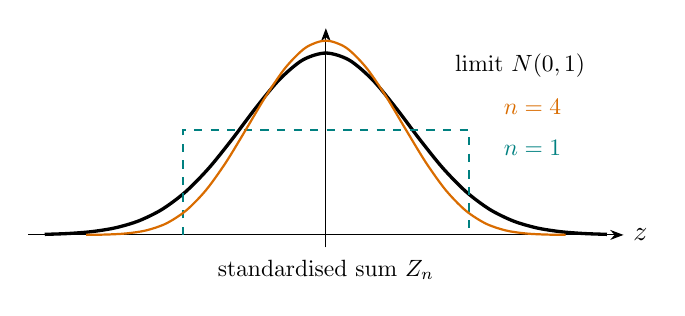
\begin{tikzpicture}[scale=1.05]
\draw[-Stealth](-3.6,0)--(3.6,0)node[right]{$z$};
\draw[-Stealth](0,-0.15)--(0,2.5);
% limiting standard normal
\draw[very thick,black,smooth,domain=-3.4:3.4,variable=\x]
  plot(\x,{2.2*exp(-0.5*\x*\x)});
% n = 1 : a flat, uniform-like standardised sum
\draw[teal,thick,dashed] (-1.732,0)--(-1.732,1.27)--(1.732,1.27)--(1.732,0);
% n = 4 : part way there
\draw[orange!85!black,thick,smooth,domain=-2.9:2.9,variable=\x]
  plot(\x,{2.35*exp(-0.62*\x*\x*(1+0.06*\x*\x))});
\node[black,scale=0.85] at (2.35,2.05) {limit $N(0,1)$};
\node[orange!85!black,scale=0.85] at (2.5,1.55) {$n=4$};
\node[teal,scale=0.85] at (2.5,1.05) {$n=1$};
\node[scale=0.85] at (0,-0.42) {standardised sum $Z_n$};
\end{tikzpicture}
\caption{Standardising removes the location and the spread, so what remains to
converge is the \emph{shape}. Even a uniform summand is close to normal by
$n=4$.}
\end{figure}


\begin{thm}[The Central Limit Theorem]
Let $\{X_n\}$ be a sequence of independent and identically distributed random variables each having mean $\mu$ and variance $\sigma^2$. Then the distribution of \hspace{0.2cm}$\frac{X_1+X_2+\dots+X_n-n\mu}{\sigma \sqrt{n}}\hspace{0.2cm}$ tends to standard normal as $n\rightarrow \infty$.\\\\ i.e for any $a\in (-\infty,\infty)$ $$P\Bigg\{\frac{X_1+X_2+\dots+X_n-n\mu}{\sigma \sqrt{n}}\leq a\Bigg\}\rightarrow \int_{-\infty}^a\frac{1}{\sqrt{2\pi}}e^{-\frac{1}{2}y^2}dy=\Phi (a)$$\\\\
\end{thm}
\begin{proof}
$$\frac{X_1+X_2+\dots+X_n-n\mu}{\sigma \sqrt{n}}=\frac{\overline{X}-\mu}{\sigma /\sqrt{n}}=\frac{\sqrt{n}(\overline{X}-\mu)}{\sigma}$$ We assume that $\mu=0$ and $\sigma^2=1$. Then \hspace{0.2cm}$\displaystyle{\frac{\sqrt{n}(\overline{X}-\mu)}{\sigma}=\sqrt{n}\overline{X}=Z_n}.$
\begin{align*}
M_{Z_n}(t) &=E\Bigg(e^{tZ_n}\Bigg)=E\Bigg(e^{t\sqrt{n}\overline{X}}\Bigg)\\
           &=E\Bigg(e^{t\sqrt{n}\frac{\sum X_i}{n}}\Bigg)\\
           &=E\Bigg(\prod^n_{i=1}e^{\frac{X_it}{\sqrt{n}}}\Bigg)\\
           &=\prod^n_{i=1}E\Bigg(e^{\frac{X_it}{\sqrt{n}}}\Bigg)\hspace{0.5cm} \text{because they are independent}\\
           &=\prod^n_{i=1}M_X(t/\sqrt{n})=\Big(M_X(t/\sqrt{n})\Big)^n\hspace{0.5cm} \text{they are identically distributed}\\
\end{align*}
$$\therefore \hspace{0.5cm} M_{Z_n}(t)=\Big(M_X(t/\sqrt{n})\Big)^n$$\\ Let $L(t)=\ln M(t)$\\
\begin{align*}
 L(0) &=\ln M(0)=0\\\\
 L'(t) &=\frac{M'(t)}{M(t)}\hspace{1cm} M(0)=1\\\\
 L'(0) &=\frac{M'(0)}{M(0)}=\mu\\\\
 L''(t) &=\frac{M''(t)M(t)-(M'(t))^2}{(M(t))^2}\\\\
 L''(0) &=\frac{E(X^2)-\big(E(X)\big)^2}{1^2}=\Var(X).
\end{align*}
$$\text{We want to show that}\hspace{0.4cm}\lim_{n\rightarrow \infty}M_{Z_n}(t)=e^{t^2/2}\hspace{0.4cm}\text{or equivalently we show that}$$ $$\lim_{n\rightarrow \infty}\ln M_{Z_n}(t)=\frac{t^2}{2}.$$\\
$$\ln M_{Z_n}(t)=n\ln M_X(t/\sqrt{n})=nL(t/\sqrt{n}).$$
\begin{align*}
\implies \hspace{0.4cm} \lim_{n\rightarrow \infty}nL(t/\sqrt{n}) &=\lim_{n\rightarrow \infty}\frac{L(t/\sqrt{n})}{1/n}\\
                                                                 &=\lim_{n\rightarrow \infty}\frac{L'\Big(\frac{t}{\sqrt{n}}\Big).(-1)t\frac{n^{-\frac{3}{2}}}{2}}{-\frac{1}{n^2}}\\
                                                                 &=\lim_{n\rightarrow \infty}\frac{tL'\Big(\frac{t}{\sqrt{n}}\Big)}{2n^{-\frac{1}{2}}}\\
                                                                 &=\frac{t}{2}\lim_{n\rightarrow \infty}\frac{L''\Big(\frac{t}{\sqrt{n}}\Big).\Big(-\frac{t}{2}\Big)n^{-\frac{3}{2}}}{-\frac{1}{2}n^{-\frac{3}{2}}}\\ 
                                                                 &=\frac{t^2}{2}\lim_{n\rightarrow \infty}L''\Big(\frac{t}{\sqrt{n}}\Big)\\
                                                                 &=\frac{t^2}{2}L'(0)=\frac{t^2}{2}\\
\end{align*}
$$\therefore \hspace{0.5cm} \lim_{n\rightarrow \infty}M_{Z_n}(t)=e^{\frac{1}{2}t^2}$$\\
The result now follows in the general case by considering the standardized random variable $Y_i=\frac{X_{i}-\mu}{\sigma}$ and apply the result above $$M_{\sqrt{n}\overline{X}}=e^{\frac{1}{2}t^2}$$ $$\sqrt{n}.\overline{Y}=\sqrt{n}.\frac{\sum\limits_{i=1}^nY_i}{n}=\sqrt{n}.\frac{\sum (X_i-\mu)}{n.\sigma}$$
$$M_{\sqrt{n}.\overline{Y}}(t)\rightarrow e^{\frac{1}{2}t^2}.$$\\
\end{proof}

\begin{note}
The proof shows that the moment generating function of $Z_n$ converges to
$e^{t^{2}/2}$, which is that of the standard normal. That alone is a statement
about \emph{functions}; what turns it into a statement about \emph{distributions}
is the continuity theorem of the chapter on generating functions. Without that
theorem the calculation above would establish nothing about $P(Z_n\leq z)$, and
it is worth being explicit that the last step of the proof is an appeal to it
rather than an observation.

The argument also assumes the moment generating function exists in a
neighbourhood of the origin, which is more than the theorem needs. The general
proof replaces $M$ by the characteristic function $\varphi(t)=E(e^{itX})$, which
always exists, and appeals to L\'evy's continuity theorem in its place. The
structure is identical.
\end{note}








\begin{remark}
Though the theorem says for each $a$.
\begin{align*}
\lim_{n\rightarrow \infty}P\Bigg\{\frac{\sqrt{n}\hspace{0.1cm}(\overline{X}-\mu)}{\sigma}\Bigg\} &=\Phi(a)\\
                       &=\int^a_{-\infty}\frac{1}{\sqrt{2\pi}}e^{-\frac{1}{2}y^2}dy
\end{align*}
It can be shown that the convergence is uniform in $a$.\\\\
Uniform convergence: $f_n(a)\longrightarrow f(a)$ $(n\rightarrow \infty)$ uniformly in $a$ if for each $\varepsilon >0\exists N \ni |f_n(a)-f(a)|<\varepsilon$ for all $a$ whenever $n>N$.\\\\
\end{remark}

\begin{exa}
The number of tourists that sign in for a trip to Victoria falls is a Poisson random variable with mean 60.\\ The company in charge of the four operators has decided that if the number signing in is 80 or more it will have two buses, whereas if the number is less than 80, it will hire only one bus. What is the probability that the company will have to hire two buses?\\\\\

Let $X$ be the number of tourists that sign in. The company will hire two buses if $x\geq 80$.
\begin{align*}
\text{The exact probability}&=P(X\geq 80)\\
&=\sum^{\infty}_{x=80}\frac{60^x\hspace{0.1cm e^{-60}}}{x!}\\
&=1-\sum^{79}_{x=0}\frac{60^x\hspace{0.1cm e^{-60}}}{x!}
\end{align*}
The computation is tidiuous, we approximate it using the central limit\\ theorem.\\\\ A Poisson with mean 60 is a sum of '60' independent Poisson each with mean 1.
$$\text{i.e}\hspace{0.5cm} X=\sum^{60}_{i=1}x_i,\hspace{0.5cm}\text{where}\hspace{0.3cm} x_i\thicksim P(1)$$
\begin{align*}
P(X\geq 80) &=P\Bigg(\sum^{60}_{i=1}x_i\geq 80\Bigg)\\\\
            &=P\Bigg\{\frac{\sum\limits^{60}_{i=1}x_i-60}{\sqrt{60}}\geq \frac{80-60}{\sqrt{60}}\Bigg\}\\\\
            &=P\Bigg\{Z\geq \frac{20}{\sqrt{60}}\Bigg\}\\\\
            &=P\{Z\geq 2.5819\}\\
            &=1-\Phi(2.58)\\
            &= \\           
\end{align*}
\end{exa}

\begin{exa}
If $10$ fair dice are rolled, find an approximate probability that the sum\\ obtained is between $40$ and $50$.\\\\
Let $X_i=$ the number for $i^{th}$ die, $$\text{then}\hspace{0.3cm} X=\sum^{10}_{i=1}x_i=\hspace{0.2cm}\text{the sum obtained}$$
$$P(40<X<50)=P\Big(40<\sum^{10}_{i=1}x_i<50\Big)$$
\begin{align*}
E(x_i) &=\sum^6_{j=1}jP(x_i=j)
       =\sum^6_{j=1}j\frac{1}{6}\\
       &=\frac{1}{6}\Big(\frac{6(6+1)}{2}\Big)\\
       &=\frac{7}{2}\\
       &=3.5\\
\end{align*}
\begin{align*}
E(x_i^2) &=\sum^6_{j=1}j^2P(x_i=j)\\ &=\sum^6_{j=1}j^2\frac{1}{6}\\
         &=\frac{1}{6}(91),\hspace{1cm}\text{from}\hspace{0.5cm}\sum^N_{x=1}x^2=\frac{(N+1)(2N+1)}{6}\\
         &=\frac{91}{6}\\
\end{align*}

$$\Var(x_i)=\frac{91}{6}-\Big(\frac{7}{2}\Big)^2=\frac{91}{6}-\frac{49}{4}=\frac{35}{12}$$\\
$$E(X)=10\times \frac{7}{2}=35$$\\  $$\Var(X)=10\times \frac{35}{12}=\frac{175}{6}$$\\
\begin{align*}
P\Bigg\{\frac{40-35}{\sqrt{175/6}}<Z<\frac{50-35}{\sqrt{175/6}}\Bigg\}
&=\Phi\Bigg(\frac{15}{\sqrt{175/6}}\Bigg)-\Phi\Bigg(\frac{5}{\sqrt{175/6}}\Bigg)\\\\
&=
\end{align*}








\pagebreak
\end{exa}


\begin{thm}[Central Limit Theorem for Independent Random Variables]
Let $\{X_n\}$ be a sequence of independent random variables having respective means $\mu_i=E(X_i)$ and $\sigma^2_i=\Var(X_i)$. If $(a)$ the $X_i's$ are uniformly bounded.\\

$\text{i.e}\hspace{0.3cm} P\{|X_i|<M\}=1\hspace{0.3cm}\text{for}\hspace{0.3cm} M\in \mathbb{R}^+\hspace{0.3cm}\text{for all}\hspace{0.3cm}i\hspace{0.3cm}\text{and}\hspace{0.3cm} \sum^{\infty}_{i=1}\sigma^2_i=\infty,$ then
\begin{align*}
\lim_{n \rightarrow \infty}P\Bigg\{\frac{\sum\limits^{n}_{i=1}(X_i-\mu_i)}{\sqrt{\sum\limits^n_{i=1}}\sigma^2_i}\leq a\Bigg\} &=\Phi(a)=\int^a_{-\infty}\frac{1}{\sqrt{2\pi}}e^{-\frac{1}{2}y^2}dy
\end{align*}
\end{thm}
Probably the best known result in probability theory is the strong law of large numbers. It states that the average of a sequence of independent random variables having a common distribution will, with probability $1$, converge to the mean of that distribution.\\\\




\begin{thm}[The Strong Law of Large Numbers]
Let $\{X_n\}$ be a sequence of independent and identically distributed random variables each having a finite mean $\mu$, then with probability $1$, \hspace{0.3cm}$\dfrac{X_1+X_2+..........+X_n}{n}\longrightarrow \mu\hspace{0.4cm} (n\longrightarrow \infty)$ $$\text{i.e}\hspace{0.3cm} P\Bigg\{\lim_{n\rightarrow \infty}\frac{X_1+X_2+..........+X_n}{n}=\mu \Bigg\}=1.$$\\
\end{thm}



\begin{proof}
We suppose that the distribution from where the sequence comes from has a finite fourth raw moment i.e $E(X^4)=M<\infty$. Also assume that $\mu=0$ i.e $E(X)=E(X_i)=0$.
$$\text{Let}\hspace{0.5cm} S_n=X_1+X_2+...........+X_n$$ 
$$E\Big(S^4_n\Big)=E\Big\{(X_1+X_2+...+X_n)(X_1+X_2+...+X_n)(X_1+X_2+...+X_n)(X_1+X_2+...+X_n)\Big\}$$
The type of terms in the expansion are five $$X^4_i,\hspace{0.2cm}X^3_iX_j,\hspace{0.2cm}X^2_iX^2_j,\hspace{0.2cm}X^1_iX_jX_l,\hspace{0.2cm} X_iX_jX_lX_k$$
$$\text{where}\hspace{0.3cm}i,j,l,k\hspace{0.3cm}\text{are different}$$
Three of the terms have expectation zero i.e
\begin{align*}
E(X^3_iX_j) &=E(X^3_i)E(X_j)=E(X^3_i).0=0\\\\
E(X^2_iX_jX_l) &=E(X_i^2)E(X_j)E(X_l)=0\\\\
E(X_iX_jX_lX_k)&=0
\end{align*}

\begin{align*}
\therefore\hspace{0.5cm} E\Big(S^4_n\Big) &=\sum^n_{i=1}E(X^4_i)+
\begin{pmatrix}
4\\2\\
\end{pmatrix}
\sum_{i\neq j}E(X^2_i)E(X^2_j)\\
&=nM+6
\begin{pmatrix}
n\\2\\
\end{pmatrix}
\Big(E(X^2)\Big)^2\\
&=nM+3n(n-1)\Big(E(X^2)\Big)^2\\\\
\implies\hspace{0.5cm} E\Big(S^4_n\Big) &=nM+3n(n-1)\Big(E(X^2)\Big)^2.................(*)
\end{align*}

\begin{align*}
0\leq \Var(X^2) &=E\Big(X^2\Big)^2-\Big(E(X^2)\Big)^2\\
                      &=E(X^4)-\Big(E(X^2)\Big)^2\\
                      &=M-\Big(E(X^2)\Big)^2\geq 0\\\\
                 \implies\hspace{0.4cm} M&\geq \Big(E(X^2)\Big)^2
\end{align*}

Then $(*)$ becomes \hspace{0.3cm}$E\Big(S_n^4\Big)\leq nM+3n(n-1)M$
\begin{align*}
E\Bigg(\frac{S_n^4}{n^4}\Bigg) &\leq \frac{M}{n^3}+\frac{3(n-1)M}{n^3}\\\\
                               &=\frac{M}{n^3}+\frac{3M}{n^2}-\frac{3M}{n^3}\\\\
                               &\leq \frac{M}{n^3}+\frac{3M}{n^2}\\
\end{align*}

$$\therefore\hspace{0.4cm}E\Bigg(\frac{S^4_n}{n^4}\Bigg)\leq \frac{M}{n^2}+\frac{3M}{n^2}\leq \frac{4M}{n^2}$$
$$\implies\hspace{0.4cm} \sum^{\infty}_{n=1}E\Bigg(\frac{S^4_n}{n^4}\Bigg)\leq 4M\sum^{\infty}_{n=1}\frac{1}{n^2}<\infty$$
$$\therefore\hspace{0.4cm} \sum^{\infty}_{n=1}E\Bigg(\frac{S^4_n}{n^4}\Bigg)<\infty$$\\
$$\implies\hspace{0.5cm} \sum^{\infty}_{n=1}\frac{S^4_n}{n^4}<\infty \hspace{0.5cm} \implies \hspace{0.5cm} \lim_{n\rightarrow \infty}\frac{S^4_n}{n^4}=0$$
$$\implies\hspace{0.5cm} \lim_{n\rightarrow \infty}\Bigg(\frac{S_n}{n}\Bigg)^4=0\hspace{0.3cm}\implies\hspace{0.3cm}\lim_{n\rightarrow \infty}\frac{S_n}{n}=0$$\\
$$\lim_{n\rightarrow \infty}\frac{X_1+X_2+..........X_n}{n}=0$$\\
$$\text{For}\hspace{0.2cm} \mu \neq 0,\hspace{0.2cm}\text{ let}\hspace{0.2cm} Y_i=X_i-\mu$$\\
$$\frac{Y_1+Y_2+........+Y_n}{n}=\frac{X_1+X_2+...........+X_n}{n}-\mu$$
$$\lim_{n\rightarrow \infty}\frac{Y_1+Y_2+..........+Y_n}{n}=0\hspace{0.4cm}\text{with probability}\hspace{0.2cm}1$$
$$\lim_{n\rightarrow \infty}\Bigg(\frac{X_1+X_2+..........+X_n}{n}-\mu\Bigg)=0$$\\
$$\implies\hspace{0.5cm}\lim_{n\rightarrow \infty}\frac{X_1+X_2+............+X_n}{n}=\mu$$
\begin{flushright}
Q.E.D
\end{flushright}
\vspace{0.5cm}
\end{proof}











\subsection{Slutsky's Theorem}

The limit theorems above concern a single sequence. In practice one almost
always meets a combination --- a quantity converging in distribution, divided by
an estimate of its standard deviation which converges in probability to a
constant. Slutsky's theorem is what licenses treating the second as though it
already were that constant, and almost every asymptotic argument in statistics
uses it.

\begin{thm}[Slutsky]
Suppose $X_n \underset{D}{\longrightarrow} X$ and
$Y_n \underset{P}{\longrightarrow} c$, where $c$ is a constant. Then
\begin{enumerate}
\item[(a)] $X_n + Y_n \underset{D}{\longrightarrow} X + c$;
\item[(b)] $X_nY_n \underset{D}{\longrightarrow} cX$;
\item[(c)] $\dfrac{X_n}{Y_n} \underset{D}{\longrightarrow} \dfrac{X}{c}$, provided $c\neq0$.
\end{enumerate}
\end{thm}

\begin{proof}
Because the limit $c$ is a constant, $Y_n \underset{P}{\longrightarrow} c$ gives
joint convergence $(X_n,Y_n)\underset{D}{\longrightarrow}(X,c)$ --- this is the
step that fails for a non-constant limit, since the marginal behaviour of two
sequences does not determine their joint behaviour. Each of the three maps
$$(x,y)\mapsto x+y,\qquad (x,y)\mapsto xy,\qquad (x,y)\mapsto x/y$$
is continuous at every point of the form $(x,c)$, the last provided $c\neq0$.
The continuous mapping theorem applied to the pair then gives the three
conclusions.
\end{proof}

\begin{note}
The requirement that $c$ be a \emph{constant} is not a technicality that can be
relaxed. If $X_n\underset{D}{\longrightarrow}X$ and
$Y_n\underset{D}{\longrightarrow}Y$ with $Y$ non-degenerate, then nothing
follows about $X_n+Y_n$ at all: take $X_n\sim N(0,1)$ and $Y_n=-X_n$, so that
each converges in distribution to $N(0,1)$, while $X_n+Y_n=0$ identically.
Taking instead $Y_n$ independent of $X_n$ gives $X_n+Y_n\sim N(0,2)$. The
marginals are the same in both cases and the limits differ, which is precisely
the point.
\end{note}

\begin{exa}
Let $X_1,\dots,X_n$ be independent and identically distributed with mean $\mu$
and finite variance $\sigma^{2}$, and let $S_n^{2}$ be the sample variance. Show
that
$$\frac{\sqrt{n}\left(\overline{X}-\mu\right)}{S_n}
\underset{D}{\longrightarrow} Z\sim N(0,1).$$
\end{exa}

\begin{solution}
By the central limit theorem,
$$\frac{\sqrt{n}\left(\overline{X}-\mu\right)}{\sigma}
\underset{D}{\longrightarrow} Z\sim N(0,1).$$
By the weak law applied to $X_i^{2}$ and to $X_i$, together with the continuous
mapping theorem, $S_n^{2}\underset{P}{\longrightarrow}\sigma^{2}$ and hence
$\sigma/S_n \underset{P}{\longrightarrow} 1$, the square root and the reciprocal
both being continuous at $\sigma^{2}>0$. Writing
$$\frac{\sqrt{n}\left(\overline{X}-\mu\right)}{S_n}
= \underbrace{\frac{\sqrt{n}\left(\overline{X}-\mu\right)}{\sigma}}_{\underset{D}{\longrightarrow}\,Z}
\ \cdot\ \underbrace{\frac{\sigma}{S_n}}_{\underset{P}{\longrightarrow}\,1},$$
part (b) of Slutsky's theorem gives the product converging in distribution to
$1\cdot Z = Z$.
\end{solution}

\begin{remark}
This example is the reason the theorem matters. The unknown $\sigma$ has been
replaced by an estimate at no asymptotic cost, and that substitution is what
makes large-sample confidence intervals and tests usable --- one does not need
to know the variance to use the normal approximation, only to estimate it
consistently. For finite $n$ under normality the exact distribution is $t$ with
$n-1$ degrees of freedom; Slutsky's theorem says the difference washes out as
$n$ grows, which is why the $t$ and normal tables agree in their lower rows.
\end{remark}


\subsection{Other Inequalities}
\begin{result}[One-Sided Chebyshev's Inequality]
If $X$ is a random variable with mean $0$ and finite variance $\sigma^2$, then for any $a>0$, \hspace{0.2cm}\\$P(X\geq a)\leq \dfrac{\sigma^2}{\sigma^2 +a^2}$
\\
\end{result}



\begin{proof}
\begin{align*}
P(X\geq a) &=P(X+k\geq a+k)\hspace{0.3cm}\text{for}\hspace{0.3cm} k>0\\ 
           &=P\Big((X+k)^2\geq (a+k)^2\Big)\\
           &\leq \frac{E(X+k)^2}{(a+k)^2}\\
           &=\frac{E(X^2+2Xk+k^2)}{(a+k)^2}\\
           &=\frac{\sigma^2+k^2}{(a+k)^2}
\end{align*}
We find a $k$ that minimizes \hspace{0.2cm}$\dfrac{\sigma^2+k^2}{(a+k)^2}$
\begin{align*}
\text{Let}\hspace{0.5cm} g(k) &=\frac{\sigma^2+k^2}{(a+k)^2}\\\\
g'(k) &=\frac{2k(a+k)^2-(\sigma^2+k^2)\hspace{0.1cm} 2(a+k)}{(a+k)^4}
\end{align*}
$$g'(k)=0\hspace{0.1cm}\Longleftrightarrow \hspace{0.1cm}k(a+k)^2-(a+k)(\sigma^2+k^2)=0$$
$$(a+k)(k(a+k)-\sigma^2-k^2)=0$$
$$(a+k)(ak-\sigma^2)=0\hspace{0.3cm}\text{either}\hspace{0.3cm}k=-a\hspace{0.3cm}\text{or}\hspace{0.3cm} k=\frac{\sigma^2}{a}$$
\begin{align*}
\therefore\hspace{0.5cm} P(X\geq a) &\leq \frac{\sigma^2+\Big(\frac{\sigma^2}{a}\Big)^2}{\Big(a+\frac{\sigma^2}{a}\Big)^2}\\\\
                                    &=\frac{\sigma^2\Big(1+\frac{\sigma^2}{a^2}\Big)}{\frac{(a^2+\sigma^2)}{a^2}}\\\\
                                    &=\frac{\sigma^2\Big(\frac{a^2+\sigma^2}{a^2}\Big)}{\frac{(a^2+\sigma^2)}{a^2}}\\
                                    &=\frac{\sigma^2}{a^2+\sigma^2}
\end{align*}
\begin{flushright}
Q.E.D
\end{flushright}
\vspace{0.3cm}
\end{proof}






\begin{exa}
In example 3.1.3, the number of items produced in a week $X$ is a random variable with mean $60$ and variance $16$. Find the bound of the production that the week's production will be fewer than $70$.
\begin{align*}
P(X<70) &=1-P(X\geq 70)\\\\
P(X\geq 70) &\leq \frac{16}{(70)^2+16}=\frac{16}{4916}\\\\
\implies\hspace{0.5cm} P(X<70) &\geq 1-\frac{16}{4916}\\\\
                               &=1-0.003255\\\\
                               &=0.996745
\end{align*}

\begin{align*}
P(X\geq a) &=P\Big(e^X\geq e^t\Big)=P\Big(e^{aX}\geq e^{at}\Big)\\
           &\leq \frac{E\Big(e^{Xt}\Big)}{e^{at}}\\
           &=\frac{M_X(t)}{e^{at}}\\\\
\implies \hspace{0.3cm} P(X\geq a) &\leq M_X(t)e^{-at}\hspace{0.5cm}t>0\\
\end{align*}
\begin{align*}
P(x\leq a) &=P\Big(e^X\leq e^a\Big)=P\Big(e^{Xt}\leq e^{at}\Big)\\
           &\leq \frac{E\Big(e^{Xt}\Big)}{e^{at}}\\
           &=E\Big(e^{Xt}\Big)e^{-at}\\\\
\implies\hspace{0.5cm} P(X\leq a) &\leq M_X(t)e^{-at}\hspace{0.3cm} \text{if}\hspace{0.3cm} t<0. \\          
\end{align*}
\end{exa}








\begin{result}[Chernoff Bounds]
If $X$ is a random variable with mgf $M_X(t)$, then for $a>0$, then we have
\begin{enumerate}
\item[(i)] $P(X\geq a)\leq e^{-at}M_X(t)$ if $t>0$.
\item[(ii)] $P(X\leq a)\leq e^{-at}M_X(t)$ if $t<0$.\\
\end{enumerate}
\end{result}









\begin{defn}
A twice differentiable real-valued function $f(x)$ is said to be 
\begin{enumerate}
\item[(i)] Convex if $f''(x)\geq 0$ for all $x$.
\item[(ii)] Concave if $f''(x)\leq 0$ for all $x$.
\end{enumerate}

$$\text{Let}\hspace{0.4cm} f(x)=x^2,\hspace{0.4cm} g(x)=e^{ax},\hspace{0.4cm} h(x)=-x^{\frac{1}{n}}$$
$$f'(x)=2x,\hspace{0.5cm}f''(x)=2;\hspace{0.5cm} f(x)=x^2\hspace{0.3cm}\text{is convex.}$$
$$K(x)=-f(x)=-x^2,\hspace{0.5cm}\text{then}\hspace{0.3cm}K(x)\hspace{0.3cm}\text{is concave.}$$
\begin{align*}
g'(x)=ae^{ax},\hspace{0.5cm}& g''(x) =a^2e^{ax}\geq 0.\\\\
&\implies\hspace{0.5cm} g(x)\hspace{0.3cm} \text{is convex}\\\\
&\implies\hspace{0.5cm} -ae^{ax}\hspace{0.3cm}\text{is concave}\\
\end{align*}
\begin{align*}
h'(x)=-\frac{1}{n}x^{\frac{1}{n}-1},\hspace{0.5cm} &h''(x)=-\frac{1}{n}\Big(\frac{1}{n}-1\Big)x^{\frac{1}{n}-2}=\frac{n-1}{n^2}x^{\frac{1}{n}-2}\\\\
&\implies\hspace{0.5cm} h(x)\hspace{0.3cm}\text{is convex}\\\\
&\implies\hspace{0.5cm} \frac{1}{n}x^{\frac{1}{n}}\hspace{0.3cm}\text{is concave}\\
\end{align*}






\pagebreak
\end{defn}

\begin{result}[Jensen's Inequality]
If $g(\cdot)$ is a convex real valued function and $X$ is random variable then \hspace{0.2cm}$E\Big(g(X)\Big)\geq g\Big(E(X)\Big).$\\
\end{result}



\begin{proof}
We expand $g(X)$ by Taylor's series at $X=\mu=E(X)$.
\begin{align*}
g(X) &=g(\mu)+g'(\mu)(X-\mu)+\frac{g''(\eta)(X-\eta)^2}{2!},\\ &{\text{where}\hspace{0.3cm}\eta \hspace{0.3cm}\text{is between}\hspace{0.3cm}X\hspace{0.3cm}\text{and}\hspace{0.3cm}\mu.}\\\\
g(X)&\geq g(\mu)+g'(\mu)(X-\mu),\hspace{0.5cm}\text{since}\hspace{0.3cm}\frac{g''(\eta)(X-\eta)^2}{2!}\geq 0.\\\\
E\Big(g(X)\Big) &\geq g(\mu)+0\\\\
\implies\hspace{0.4cm} E\Big(g(X)\Big)&\geq g(\mu)=g\Big(E(X)\Big).\\\\
\end{align*}















\pagebreak
\end{proof}

\subsection{Practice Problems}

\begin{problem}
Let $X_1,\dots,X_n$ be independent with mean $\mu$ and variance $\sigma^{2}$.
Use Chebyshev's inequality to show that $\overline{X}\underset{P}{\longrightarrow}\mu$,
and find how large $n$ must be so that
$P\left(\left|\overline{X}-\mu\right|\geq 0.1\sigma\right)\leq 0.05$.
\end{problem}
\begin{solution}
Since $\Var\left(\overline{X}\right) = \sigma^{2}/n$, Chebyshev gives
$$P\left(\left|\overline{X}-\mu\right|\geq\varepsilon\right)
\leq \frac{\sigma^{2}}{n\varepsilon^{2}} \longrightarrow 0 ,$$
which is the weak law. Setting $\varepsilon = 0.1\sigma$,
$$\frac{\sigma^{2}}{n(0.1\sigma)^{2}} = \frac{100}{n} \leq 0.05
\quad\Longrightarrow\quad n \geq 2000 .$$

Chebyshev is deliberately crude. The central limit theorem gives
$1.96\sigma/\sqrt{n} = 0.1\sigma$, that is $n\approx 385$ --- about a fifth as
many. The bound holds for every distribution with finite variance, which is what
it is paying for.
\end{solution}

\begin{problem}
Let $X$ be a random variable that takes only nonnegative values. Prove that for
any $a>0$,
$$P(X\geq a)\leq\frac{E(X)}{a}.$$
\end{problem}
\begin{solution}
Take $X$ continuous with density $f$, which is zero on $x<0$. Then
\begin{align*}
E(X) &= \int_0^{\infty}xf(x)\,dx
= \int_0^{a}xf(x)\,dx + \int_a^{\infty}xf(x)\,dx\\
&\geq \int_a^{\infty}xf(x)\,dx\\
&\geq \int_a^{\infty}af(x)\,dx = aP(X\geq a).
\end{align*}
The first inequality drops a nonnegative integral; the second uses $x\geq a$ on
the range of integration. Dividing by $a>0$,
$$P(X\geq a)\leq\frac{E(X)}{a}.$$
The discrete case is the same argument with sums in place of integrals; the
indicator proof given for Markov's inequality in the text covers both at once.
\end{solution}

\begin{problem}
Let $X$ be a random variable with mean $\mu$ and variance $\sigma^{2}$. Prove
that for any $k>0$,
$$P\left(|X-\mu|\geq k\right)\leq\frac{\sigma^{2}}{k^{2}}.$$
\end{problem}
\begin{solution}
Since $(X-\mu)^{2}\geq0$, Markov's inequality applies to it with $a=k^{2}$:
$$P\left((X-\mu)^{2}\geq k^{2}\right)\leq\frac{E\left[(X-\mu)^{2}\right]}{k^{2}}.$$
Since $(X-\mu)^{2}\geq k^{2}$ if and only if $|X-\mu|\geq k$,
$$P\left(|X-\mu|\geq k\right)\leq\frac{E\left[(X-\mu)^{2}\right]}{k^{2}}
= \frac{\sigma^{2}}{k^{2}}.$$
\end{solution}

\begin{problem}
Let $X_1,X_2,\dots,X_n$ be independent and identically distributed random
variables with a finite mean $\mu$. Prove that the sample mean $\overline{X}_n$
converges in probability to $\mu$.
\end{problem}
\begin{solution}
Write $\sigma^{2}$ for the common variance, taken to be finite. Then
$$\overline{X}_n = \frac{X_1+X_2+\cdots+X_n}{n},\qquad
\Var\left(\overline{X}_n\right) = \frac{\sigma^{2}}{n}.$$
By Chebyshev's inequality, for any $\varepsilon>0$,
$$P\left(\left|\overline{X}_n-\mu\right|\geq\varepsilon\right)
\leq\frac{E\left[\left(\overline{X}_n-\mu\right)^{2}\right]}{\varepsilon^{2}}
= \frac{\Var\left(\overline{X}_n\right)}{\varepsilon^{2}}
= \frac{\sigma^{2}}{n\varepsilon^{2}}.$$
Therefore
$$\lim_{n\rightarrow\infty}P\left(\left|\overline{X}_n-\mu\right|\geq\varepsilon\right)
\leq\lim_{n\rightarrow\infty}\frac{\sigma^{2}}{n\varepsilon^{2}} = 0 ,$$
that is, $\overline{X}_n\underset{P}{\longrightarrow}\mu$.

The question assumes only a finite mean. The conclusion still holds then ---
that is Khinchin's form of the weak law --- but its proof needs a truncation
argument. A finite variance is what lets Chebyshev do all the work here.
\end{solution}

\begin{problem}
Let $X_1,X_2,\dots,X_n$ be independent Bernoulli random variables with
probability $p$, and let $Y_n = \frac1n\sum_{k=1}^{n}X_k$. Show that
$Y_n\underset{P}{\longrightarrow}p$.
\end{problem}
\begin{solution}
Since $E(X_k)=p$ and $\Var(X_k)=p(1-p)$,
$$E(Y_n) = \frac1n\sum_{k=1}^{n}E(X_k) = \frac{np}{n} = p$$
and
$$\Var(Y_n) = \frac{1}{n^{2}}\sum_{k=1}^{n}\Var(X_k)
= \frac{1}{n^{2}}\,np(1-p) = \frac{p(1-p)}{n}.$$
By Chebyshev's inequality, for any $\varepsilon>0$,
$$P\left(|Y_n-p|\geq\varepsilon\right)\leq\frac{\Var(Y_n)}{\varepsilon^{2}}
= \frac{p(1-p)}{n\varepsilon^{2}}\longrightarrow0\qquad(n\rightarrow\infty).$$
Therefore $Y_n\underset{P}{\longrightarrow}p$: the proportion of successes
converges to the probability of success.

As set, the question wrote $Y_n=\sum_{k=1}^{n}X_k$ with limit $\mu$. The sum
itself has mean $np$ and does not converge; it is the average that does, and its
limit is the common mean $p$.
\end{solution}

\begin{problem}
Let $X_1,X_2,\dots,X_{20}$ be independent UNIF$(0,1)$ random variables. Find
normal approximations for each of the following:
\begin{enumerate}[label=(\alph*)]
\item $P\left(\sum_{i=1}^{20}X_i\leq12\right)$;
\item the 90th percentile of $\sum_{i=1}^{20}X_i$.
\end{enumerate}
\end{problem}
\begin{solution}
Let $S=\sum_{i=1}^{20}X_i$. Each $X_i$ has
$$E(X_i) = \frac{0+1}{2} = \frac12,\qquad
\Var(X_i) = \frac{(1-0)^{2}}{12} = \frac{1}{12},$$
so $E(S) = 20\times\frac12 = 10$ and $\Var(S) = 20\times\frac{1}{12} = \frac53$.

\subhead{(a)}
By the central limit theorem,
$$P(S\leq12) = P\left(\frac{S-E(S)}{\sigma_S}\leq\frac{12-10}{\sqrt{5/3}}\right)
\approx P(Z\leq1.549)\approx0.9393 .$$

\subhead{(b)}
We want the $x$ with $P(S\leq x) = 0.90$:
$$P\left(Z\leq\frac{x-10}{\sqrt{5/3}}\right) = 0.90
\quad\Longrightarrow\quad
\frac{x-10}{\sqrt{5/3}} = \Phi^{-1}(0.90) = 1.2816 .$$
Hence
$$x = 10+1.2816\sqrt{5/3}\approx11.65 .$$
\end{solution}


\section{ADDITIONAL TOPICS IN PROBABILITY}
\vspace{0.5cm}
\subsection{Stochastic Processes}

Everything so far has concerned single random variables, or finite collections
of them. A stochastic process is an indexed family, and the index is almost
always time. The shift of view is what the rest of this section rests on, and
the vocabulary is worth fixing before the particular processes appear.

\begin{defn}
A \emph{stochastic process} is a collection $\{X_t : t\in T\}$ of random
variables defined on a common probability space and indexed by a set $T$. The
set $T$ is the \emph{index set}, usually interpreted as time; the set of values
the $X_t$ can take is the \emph{state space}.
\end{defn}

\begin{note}
Four combinations arise, and a process is classified by which it is:
\begin{enumerate}
\item[$-$] $T$ countable and the state space countable --- a Markov chain on a
finite or countable set, for instance;
\item[$-$] $T$ countable, state space continuous --- a time series of real
measurements;
\item[$-$] $T$ an interval, state space countable --- the Poisson process
counting arrivals;
\item[$-$] $T$ an interval, state space continuous --- Brownian motion.
\end{enumerate}
A process with $T = \{0,1,2,\dots\}$ is called a \emph{discrete-time} process; a
process with $T = [0,\infty)$ a \emph{continuous-time} one.
\end{note}

\begin{defn}
A \emph{realisation}, or \emph{sample path}, of the process is the function
$t\mapsto X_t(\omega)$ obtained by fixing one outcome $\omega$. The process is
the collection of all such paths together with the probabilities attached to
them.
\end{defn}

\begin{remark}
The distinction between a process and its paths is the one that causes most
trouble. A statement such as ``$X_t\rightarrow0$'' is ambiguous until one says
whether it concerns the paths, which is almost sure convergence, or the
distributions, which is convergence in distribution --- exactly the modes
distinguished in the previous chapter, now applied along a time index. The four
modes were not an abstract exercise; they are the language this section needs.
\end{remark}

\subhead{Properties a process may have}

\begin{defn}
Let $\{X_t\}$ be a stochastic process.
\begin{enumerate}
\item[(i)] It has \emph{independent increments} if for
$t_0<t_1<\cdots<t_n$ the differences
$X_{t_1}-X_{t_0},\ \dots,\ X_{t_n}-X_{t_{n-1}}$ are independent.
\item[(ii)] It has \emph{stationary increments} if the distribution of
$X_{t+s}-X_{t}$ depends on $s$ but not on $t$.
\item[(iii)] It is \emph{strictly stationary} if the joint distribution of
$\left(X_{t_1+h},\dots,X_{t_n+h}\right)$ does not depend on $h$.
\item[(iv)] It is \emph{weakly} or \emph{second-order stationary} if $E(X_t)$ is
constant and $\Cov\left(X_t,X_{t+s}\right)$ depends on $s$ alone.
\item[(v)] It has the \emph{Markov property} if the future depends on the past
only through the present:
$$P\left(X_{t_{n+1}}\in A \mid X_{t_1},\dots,X_{t_n}\right)
= P\left(X_{t_{n+1}}\in A \mid X_{t_n}\right).$$
\end{enumerate}
\end{defn}

\begin{note}
Strict stationarity implies weak stationarity whenever the second moments exist,
but not conversely --- weak stationarity constrains only the first two moments
and says nothing about the rest of the distribution. The one case where they
coincide is the Gaussian process, because a joint normal distribution is
determined by its mean vector and covariance matrix and by nothing else.
\end{note}

\subhead{Some standard processes}

\begin{exa}[White noise]
A sequence $\{\varepsilon_t\}$ of uncorrelated random variables with constant
mean zero and constant variance $\sigma^{2}$. It is weakly stationary by
construction, and it is the building block from which the processes below are
assembled.
\end{exa}

\begin{exa}[Random walk]
Let $\{\varepsilon_t\}$ be independent with mean zero and variance
$\sigma^{2}$, and set $X_0=0$, $X_n = \sum_{i=1}^{n}\varepsilon_i$. Then
$$E(X_n) = 0,\qquad \Var(X_n) = n\sigma^{2},$$
so the process has independent and stationary increments and the Markov
property, but it is \emph{not} stationary: its variance grows without bound. A
random walk wanders away rather than settling, which is why differencing rather
than averaging is the tool used on such series.
\end{exa}

\begin{exa}[Counting process]
A process $\{N_t : t\geq0\}$ taking non-negative integer values, with $N_0=0$
and $N_s\leq N_t$ whenever $s\leq t$, so that $N_t$ counts the events occurring
in $[0,t]$. If it has independent and stationary increments and the number of
events in an interval of length $t$ is POI$(\lambda t)$, it is the \emph{Poisson
process}, which the next subsection treats in detail.
\end{exa}

\begin{remark}
The three properties above --- independent increments, stationary increments and
the Markov property --- are what make a process tractable, and the Poisson
process has all three. That is the whole reason it occupies the place it does:
not that arrivals in the world are especially Poisson, but that a process with
those three properties and integer values is forced to be Poisson, so the
assumptions are checkable even when the conclusion cannot be observed directly.
\end{remark}


\subsection{Poisson Process}
\begin{defn}
A function $f(x)$ is said to be $O(h)$ if \hspace{0.2cm}$\displaystyle{\lim_{h\rightarrow 0}\frac{f(x)}{h}=0}$\\

i.e $f$ is $O(h)$ if for small values of $h$, $f(h)$ is small in relation to $h$. For example $\dfrac{e^{-1/x}}{1/x}$ say $h=1/10$ then $\dfrac{e^{-1/10}}{1/10}$, thus $h\rightarrow 0$ as $x\rightarrow \infty$.\\ 

Suppose that "events" occur at random time points and let $N(t)$ denote the number of events that occur in a time interval $[0,t]$.\\
\end{defn}



\begin{defn}
The collection of random variables $\{N(t),\hspace{0.1cm}t\geq 0\}$ is said to be a Poisson process with rate $\lambda$, $\lambda >0$ if
\begin{enumerate}
\item[i.] $N(0)=0$
\item[ii.] The number of events that occur in disjoint time intervals are \\independent.
\item[iii.] The distribution of the number of events that occur in a given time interval depends only on the length of that interval.
\item[iv.] $P\{N(t)=1\}=\lambda h+O(h)$
\item[v.] $P\{N(t)\geq 2\}=O(h)$\\
\end{enumerate}
\end{defn}





\begin{remark}
Condition (i): process starts at time zero.\\
Condition (ii): independent $(t,t+s)$, $(t+k,t+b)$ where $k>s$ and $b>k$


\begin{figure}[H]
\centering
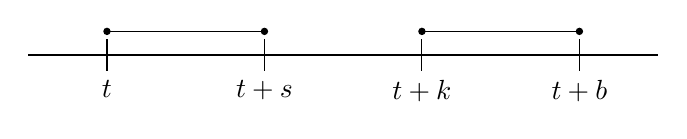
\begin{tikzpicture}[=>stealth]
\draw(-4,0)--(4,0)
(1,0.2)--(1,-0.2)
(-1,0.2)--(-1,-0.2)
(3,0.2)--(3,-0.2)
(-3,0.2)--(-3,-0.2)
(-3,0.3)node[shape=circle,fill,scale=0.01cm]{}
(-1,0.3)node[shape=circle,fill,scale=0.01cm]{}
(3,0.3)node[shape=circle,fill,scale=0.01cm]{}
(1,0.3)node[shape=circle,fill,scale=0.01cm]{}
(-3,0.3)--(-1,0.3)
(1,0.3)--(3,0.3)
(-3,-0.2)node[below]{$t$}
(-1,-0.2)node[below]{$t + s$}
(1,-0.2)node[below]{$t+k$}
(3,-0.2)node[below]{$t+b$};
\end{tikzpicture}
\end{figure}
\end{remark}


\begin{lem}
$\text{For a Poisson process with rate}\hspace{0.3cm} \lambda,\hspace{0.3cm} P\{N(t)=0\}=e^{-\lambda t}.$\\
\end{lem}


\begin{proof}
$\text{Denote}\hspace{0.4cm} P_0(t)=P\{N(t)=0\}.$
\begin{align*}
P_0(t+h) &=P\{N(t+h)=0\}\\
         &=P\{N(t)=0,\hspace{0.1cm} N(t+h)-N(t)=0\}\\
         &=P\{N(t)=0\}\hspace{0.1cm} P\{N(t+h)-N(t)=0\}\\
         &=P_0(t)\hspace{0.1cm} P\{N(h)=0\}\\
         &=P_0(t)\hspace{0.1cm} (1-\lambda h+O(h))\\
         &=P_0(t)-\lambda hP_0(t)-O(h)
\end{align*} 
\begin{align*}
P_0(t+h)-P_0(t) &=-\lambda hP_0(t)-O(h)\\\\
\frac{P_0(t+h)-P_0(t)}{h} &=-\lambda P_0(t)-\frac{O(h)}{h}\\\\
\lim_{h\rightarrow 0}\frac{P_0(t+h)-P_0(t)}{h} &=-\lambda P_0(t)-\lim_{h\rightarrow 0}\frac{O(h)}{h}\\\\
\therefore\hspace{0.4cm} P'_0(t) =-\lambda P_0(t)\hspace{0.5cm}&\implies\hspace{0.5cm} \frac{P'_0(t)}{P_0(t)}=-\lambda
\end{align*}
\begin{align*}
\int\frac{P'_0(t)}{P_0(t)}dt &=-\int\lambda dt\\\\
\implies\hspace{0.5cm} \ln P_0(t) &=-\lambda t+c\\\\
\implies\hspace{0.5cm} P_0(t) &=ke^{-\lambda t},\hspace{0.4cm} \text{where}\hspace{0.3cm} k=e^c
\end{align*}
$$P_0(t)=ke^{-\lambda t}$$ $$t=0,\hspace{0.5cm} P_0(0)=k,\hspace{1cm} \therefore\hspace{0.3cm} k=1$$
$$\therefore\hspace{0.5cm} P_0(t)=e^{-\lambda t}$$ $$\implies\hspace{0.5cm} P\{N(t)=0\}=e^{-\lambda t}.$$\\

Denote $T_n$ to be the time elapsed between the $(n-1)^{\text{th}}$ event and the $n^{\text{th}}$ event.
The sequence $\{T_n\}$ is called the sequence of inter arrival times.  For example, if $T_1=4$ and $T_2=12$, then the first event occurred at time $4$ units and the second event occurred at time $16$.



\begin{figure}[H]
\centering
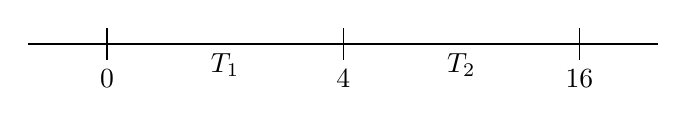
\begin{tikzpicture}[=>stealth]
\draw(-4,0)--(4,0)
(0,0.2)--(0,-0.2)
(-3,0.2)--(-3,-0.2)
(3,0.2)--(3,-0.2)
(-3,-0.2)node[below]{$0$}
(0,-0.2)node[below]{$4$}
(3,-0.2)node[below]{$16$}
(-1.5,0)node[below]{$T_1$}
(1.5,0)node[below]{$T_2$};
\end{tikzpicture}
\end{figure}










\begin{align*}
P(T_1>t) &=P\{N(t)=0\}=e^{-\lambda t}\\\\
\implies\hspace{0.5cm} P(T_1\leq t) &=1-e^{-\lambda t}\hspace{0.3cm}\implies\hspace{0.3cm} T_1\hspace{0.3cm}\text{is exponential with mean}\hspace{0.3cm} \frac{1}{\lambda}.\\\\
\therefore\hspace{0.5cm} P(T_2>s) &=E\Big(\frac{P(T_2>s)}{T_1}\Big).\\\\
P(T_2>s \mid T_1=t) &=P(\text{no event in the interval}\hspace{0.3cm} (t,t+s))\\\\
               &=P(N(s)=0)\\\\ &=e^{-\lambda s}
\end{align*}
$T_2$ has an exponential distribution with mean $1/\lambda$.\\\\
$\therefore$ it follows that $T_n$ is exponential with mean $1/\lambda$, $n=1,2,.......,n$\\\\
\end{proof}

\begin{result}
Let $\{T_n\}$ be a sequence of inter arrival times of a Poisson process, then $T_1,T_2,..........$ are independent identically distributed as exponential with mean $1/\lambda$.\\\\ Denote the arrival of the $n^{\text{th}}$ event by $S_n$, which is the waiting time until the $n^{\text{th}}$ event occurs $$\text{i.e}\hspace{0.5cm}S_n=\sum^n_{i=1}T_i$$ What is the distribution of $S_n$?\\\\ Since it is a sum of $iid$ $g(1,\lambda)$
\begin{align*}
\therefore\hspace{0.3cm} f_{S_m}(x) &=\frac{\lambda^n\hspace{0.1cm} x^{n-1}\hspace{0.1cm} e^{-\lambda x}}{\Gamma(n)}\\\\
                                    &\frac{(\lambda x)^{n-1}\hspace{0.1cm}\lambda \hspace{0.1cm} e^{-\lambda x}}{(n-1)!},\hspace{0.5cm} x>0
\end{align*}
We want $P\{N(t)=n\}$.\\\\
\end{result}


\begin{thm}
For a Poisson process with rate $\lambda$, $N(t)=$ the number of events that occur in time interval $[0,t]$, $$P\{N(t)=n\}=\frac{(\lambda t)^n\hspace{0.1cm e^{-\lambda t}}}{n!},\hspace{0.5cm} n=0,1,........, n$$
\end{thm}

\begin{proof}
For a Poisson process with rate $\lambda$,  $N(t)=$ the number of event in time interval $[0,t]$.  The $n^{\text{th}}$ event will only occur before or at time $t$. If and only the number of events that occur by time $t$ is at atleast $n$ i.e $N(t)\geq n$.$$S_n=T_1+T_2+.........+T_n=\sum^n_{i=1}T_i$$ $$\text{then we have}\hspace{0.5cm} N(t)\geq n \Longleftrightarrow S_n\leq t.$$
\begin{align*}
P\{N(t)=n\} &=P\{N(t)\geq n\}-P\{N(t)\geq n+1\}\\
            &=P\{S_n\leq t\}-P\{S_{n+1}\leq t\}\\\\
            &=\int^t_0\frac{(\lambda x)^{n-1}\lambda e^{-\lambda x}}{(n-1)!}dx-\int^t_0\frac{(\lambda x)^n\lambda e^{-\lambda x}}{n!}dx\\\\
            &=\int^t_0\frac{(\lambda x)^{n-1}\lambda e^{-\lambda x}}{(n-1)!}dx-\Bigg(\frac{(\lambda x)^n}{n!}\hspace{0.1cm}\lambda(-1)\frac{e^{-\lambda x}}{\lambda}\Bigg|^t_0+\int^t_0\frac{d}{dx}(\lambda x)^n\frac{e^{-\lambda x}}{n!}dx
\end{align*}
\begin{align*}
\implies\hspace{0.5cm} P\{N(t)=n\} &=\int^t_0\frac{(\lambda x)^{n-1}\lambda e^{-\lambda x}}{(n-1)!}dx+\frac{(\lambda t)^ne^{-\lambda t}}{n!}-0-\int^t_0\frac{(\lambda x)^{n-1}\lambda e^{-\lambda x}}{(n-1)!}dx\\\\
&=\frac{(\lambda t)^ne^{-\lambda t}}{n!} 
\end{align*}
\begin{flushright}
Q.E.D\\
\end{flushright}

\vspace{0.5cm}
\end{proof}









\begin{exa}
If it was reported that an insurance company with a $24$ hour hot line, the claims followed a Poisson process with rate of $4$ claims per day. Find the following
\begin{enumerate}
\item[i.] probability that more than $2$ claims were being reported on a given day.
\item[ii.] the time until the next reported claim is more than an hour.\\
\end{enumerate}
\begin{enumerate}
\item[i.]
\begin{align*}
P(N(t)>2) &=1-P\{N(t)\leq 2\}\\
          &=1-\sum^2_{k=0}\frac{4^ke^{-4}}{k!}\\
          &=1-e^{-4}\Big(1+4+\frac{4^2}{2}\Big)\\
          &=1-13e^{-4}\\
          &=0.7619
\end{align*}
\item[ii.]
\begin{align*}
P(T>1),&\hspace{0.5cm} T\thicksim \exp\Big\{\frac{4}{24}\Big\}=\exp\Big\{\frac{1}{6}\Big\}\\
&\implies\hspace{0.4cm} E(T)=6\\\\
P(T>1)&=e^{-\lambda}=e^{-1/6}
\end{align*}
\end{enumerate}












\pagebreak
\end{exa}
\subsection{Markov Chains (Sequence of Dependent Trials)}
We have been studying sequences of independent trials (Binomial, Poisson, Geometric e.t.c). We think of an experiment having finite or countable set of outcomes and we keep repeating the experiment. Denote by $X_n$, the outcome of the $n^{\text{th}}$ trial. Let $\{0,1,2,.....,m\}$ be the possible values $X_n$ can take. We interpret $X_n$ as being the state of some system at time $n$. Thus we say that the system is in state $i$ at some time $n$ if $X_n=i$.\\\\
The sequence of random variables is said to form Markov Chain if each time the system is in state $i$ there is some fixed probability call it $P_{ij}$ that the system will next be is state $j$ (at time $n+1$)
\begin{align*}
&P\{X_{n+1}=j/X_n=i,X_{n-1}=i_{n-1},X_{n-2}=i_{n-2},.........,X_1=i_1, X_0=i_0\}\\ &=P\{X_{n+1}=j/X_{n}=i\}\\ &=P_{ij}\\
\end{align*}

\begin{remark}
\begin{enumerate}
\item The conditional probabilities \hspace{0.2cm}$P\{X_{n+1}=j/X_n=i\}=P_{ij}\hspace{0.2cm}$ are called transition probabilities of the Markov chain.
\item Markov chain having stationary transition probabilities i.e $P\{X_{n+1}=j/X_n=i\}=P_{ij}$ is independent of $n$.
\item If we say that the sequence of random variables $\{X_n\}$, $n\geq 0$ form a Markov chain, we mean that that $X_n$'s satisfy the Markov property and hence stationary transition probabilities.
\item The Markov property is when given that the system is in the present state, the past states have no influence on the future i.e
\begin{align*}
&P\{X_{n+1}=j/X_n=i, X_{n-1}=i_{n-1}, X_{n-2}=i_{n-2}, .........., X_1=i_1, X_0=i_0\}\\
&=P\{X_{n+1}=j/ X_n=i\}
\end{align*}
\item The study of Markov chains is worth while as it has rich theory and there are a large number of systems arising in practice that can be modeled by Markov chains. Markov chains have many useful applications.\\
\end{enumerate}

If the possible states of a Markov chain are $0,1,2,........,m$ then \hspace{0.3cm}$\sum\limits^m_{j=0}P_{ij}=1,\hspace{0.5cm} P_{ij}\geq 0\hspace{0.2cm}$
It is convenient to arrange the transition probabilities in a square matrix known as the transition probability matrix
$$P=
\begin{bmatrix}
P_{00}&P_{01}&P_{02}&..........&P_{0m}\\
P_{10}&P_{11}&&&\\
.&.&&&\\
.&.&&&\\
.&.&&&\\
.&.&&&\\
P_{m0}&P_{m1}&&..........&P_{mm}\\
\end{bmatrix}
$$
The joint probability mass function of $X_1...........X_n$ is given by 
\begin{align*}
&P\{X_n=i_n, X_{n-1}=i_{n-1}, .........., X_0=i_0\}\\\\
&=P\{X_n=i_n/X_{n-1}=i_{n-1}, ...., X_0=i_0\}\hspace{0.1cm}\times\hspace{0.1cm} P\{X_{n-1}=i_{n-1}, X_{n-2}=i_{n-2},...., X_0=i_0\}\\\\
&=P\{X_n=i_n/X_{n-1}=i_{n-1}\}\hspace{0.1cm}P\{X_{n-1}=i_{n-1}/X_{n-2}=i_{n-2}\}\hspace{0.1cm}P\{X_{n-2}=i_{n-2}/X_{n-3}=i_{n-3}\}.....\\&............P\{X_1=i_1/X_0=i_1\}\\\\
&=P_{i_{n-1}i_n},\hspace{0.2cm} P_{i_{n-2}i_{n-1}},\hspace{0.2cm}P_{i_{n-3}i_{n-2}}.............P_{i_0i_1}\hspace{0.2cm} P(X_0=i_0)\\\
\end{align*}
\end{remark}

\begin{exa}
Consider a gambler who at each play of the game either wins $1$ unit with probability $P$ or loses $1$ unit with probability $1-P$. If we suppose that the gambler will stop playing when his fortune hits either $0$ or $m$, then the \\gambler's sequence of fortunes is a Markov chain having transition\\ probabilities.\\\\
$$P_{i,i+1}=P,\hspace{0.3cm} P_{i,i-1}=1-P,\hspace{0.3cm} i=1,2,........, m-1.$$ $$P_{00}=1,\hspace{0.5cm} P_{mm}=1$$\\
$$
\begin{bmatrix}
1&0&0&0&0&0&0\\
1-P&0&P&0&0&0&0\\
0&1-P&0&P&0&0&0\\
0&0&1-P&0&P&0&0\\
0&0&0&1-P&0&P&0\\
0&0&0&0&1-P&0&P\\
0&0&0&0&0&0&1\\
\end{bmatrix}
$$\\
$$P_{ij}=P\{X_{n+1}=j/X_n=i\}$$

$$P^{(2)}_{ij}=P\{X_{n+1}=j/X_n=i\}=\text{the system in state}\hspace{0.2cm}i\hspace{0.2cm}\text{will be in state}\hspace{0.2cm} j\hspace{0.2cm}\text{after two transitions.}$$\\
We want to compute $P^{(2)}_{ij}!$
$$P^{(2)}_{3,4}=P\{X_{n+2}=4/X_n=3\}=0$$
\begin{align*}
P^{(2)}_{ij} &=P\{X_{n+2}=j/X_n=i\}\\
             &=P\{X_2=j/X_0=i\}\\
             &=\sum^m_{k=0}P\{X_2=j/X_1=k,X_0=i\}\hspace{0.1cm}P\{X_1=k/X_0=i\}\\
             &=\sum^m_{k=0}P\{X_2=j/X_1=k\}\hspace{0.1cm}P\{X_1=k/X_0=i\}\\
             &=\sum^m_{k=0}P_{kj}P_{ik}
             =\sum^m_{k=0}P_{ik}\hspace{0.1cm}P_{kj}\\\\
\implies\hspace{0.5cm}P^{(2)}_{ij} &=\sum^m_{k=0}P_{ik}P_{kj}\\
\end{align*}
\begin{align*}
P^{(2)}_{3,5} &=\sum^6_{k=0}P_{3k}P_{k5}\\
              &=P_{30}P_{05}+P_{31}P_{15}+P_{32}P_{25}+.....\\
              &=P^2
\end{align*}

$$P^{(2)}_{34}=\sum^6_{k=0}P_{3k}P_{k4}=0.$$\\
In general, we can define $n$-stage transition probabilities, denoted by $P^{(n)}_{ij}$ and is given by $$P^{(n)}_{ij}=P\{X_{n+l}=j/X_l=i\}=P\{X_n=j/X_0=i\}$$\\






\pagebreak
\end{exa}

\begin{thm}[The Chapman-Kolmogrov Equation]
$$P^{(n)}_{ij}=\sum^m_{k=0}P^{(r)}_{ik}P^{(n-r)}_{kj}\hspace{1cm} 0<r<n.$$
\end{thm}
\begin{proof}
\begin{align*}
P^{(n)}_{ij} &=P\{X_{n+l}=j/X_l=i\}\\
             &=P\{X_n=j/X_0=i\}\\\\
             &=\sum^m_{k=0}P\{X_n=j/X_r=k, X_0=i\}\hspace{0.1cm} P\{X_r=k/X_0=i\}\\\\
             &=\sum^m_{k=0}P\{X_n=j/X_r=k\}P\{X_r=k/X_0=i\}\\\\
   P^{(n)}_{ij}&=\sum^m_{k=0}P^{(n-r)}_{kj}P^{(r)}_{ik}\\\\
\implies\hspace{0.5cm}   P^{(n)}_{ij}&=\sum^m_{k=0}P^{(r)}_{ik}P^{(n-r)}_{kj} \\         
\end{align*}
\end{proof}

\begin{exa}[Random Walk]
Tracking a particle as it moves along one-dimensional axis. Suppose that at each point in time the particle will move either one-step to the right or one-step to the left with probabilities $P$ and $1-P$ respectively.\\ The particles path follows a Markov chain with transition probabilities$$P_{i,i+1}=P\hspace{0.4cm} \text{and}\hspace{0.4cm} P_{i,i-1}=1-P,\hspace{1cm} i=0,\pm 1,\pm 2,\pm 3..........$$
If the particle is in state $i$, then the probability that it will be in state $j$ after  $$n\hspace{0.3cm}\text{ transitions is that}\hspace{0.3cm} \frac{n-i+j}{2}\hspace{0.3cm}\text{ steps are to the right and}$$ $$n-\frac{(n-i+j)}{2}=\frac{n+i-j}{2}\hspace{0.4cm}\text{are to the left.}$$
$$P^{(n)}_{ij}=
\begin{pmatrix}
n\\\\\frac{n-i+j}{2}\\
\end{pmatrix}
P^{\frac{n-i+j}{2}}(1-P)^{\frac{n+i-j}{2}}\hspace{0.2cm}............\hspace{0.2cm} (*)
$$
where $
\begin{pmatrix}
n\\x\\
\end{pmatrix}
=0$ if $x$ is not a non-negative integer less than or equal to $n$ \\\\$*$ can be written as 
\begin{align*}
P^{(2n)}_{i,i+2k} &=
\begin{pmatrix}
2n\\\\ n+k\\
\end{pmatrix}
P^{n+k}(1-P)^{n-k},\hspace{0.5cm} k=0, \pm 1, \pm 2,........,\pm n\\\\
P^{(2n+1)}_{i,i+2k+1} &=
\begin{pmatrix}
2n+1\\\\n+k+1\\
\end{pmatrix}
P^{n+k+1}(1-P)^{n-k},\hspace{0.5cm} k=0, \pm 1, \pm 2,.........,\pm n.\\\\
P\{X_n=j\} &=\sum^n_{i=1}P(X_n=j \mid X_0=i)P(X_0=i)\\
           &=\sum_i P^{(n)}_{ij} P(X_0=i)
\end{align*}
$P^{(n)}_{ij}$ converges as $n\longrightarrow \infty$ to the value $\pi_j$ that depends only on $j$. That is for large values of $n$ the probability
of being in state $j$ after $n$ transitions is approximately equal to $\pi_j$ regardless of the initial state it was.\\\\
It can be shown that a sufficient condition for a Markov chain to posses this property is that $n>0$,$$P^{(n)}_{ij}>0,\hspace{0.3cm}\text{for}\hspace{0.3cm} i,j=0,1,2,.........., m\hspace{0.2cm}........(**)$$ A Markov chain that satisfy $(**)$ are said to be ergodic chains.\\



\textbf{Comments}:\\
Transition functions and initial distributions.\\Let $\{X_n\}$, $n\geq 0$ be a Markov chain having state space $\mathbf{E}$.
\begin{enumerate}
\item The function $P_{ij}$, $i\in \mathbf{E}$ and $j\in \mathbf{E}$ defined by \hspace{0.2cm}$P_{ij}=P\{X_1=j/X_0=j\},\hspace{0.5cm} i,j\in \mathbf{E}\hspace{0.2cm}$ is called the transition function of the Markov chain. It is such that $P_{ij}\geq 0$ and $\sum\limits^m_{j=1}P_{ij}=1$.
\item The function $\pi_0(i)=P\{X_0=i\}$, is called  the initial distribution, it is such that $\pi_0(i)\geq 0$ and $\sum\limits^m_{i=1}\pi_0=0$.
\item It can be shown that given any transition function and any initial distributions, there is a probability space and random variables $X_n$, $n\geq 0$ defined as on the probability space satisfying the following
\begin{align*}
&P\{X_n=i_n, X_{n-1}=i_{n-1},.............,X_1=i_1, X_0=i_0\}\\
&=P_{i_{n-1}i_n} P_{i_{n-2}i_{n-1}} ........... P_{i_1i_2} P_{i_0i_1} \pi_0 (i_0)
\end{align*}
\end{enumerate}
\end{exa}


\begin{defn}
The hitting Time $T_j$ of state $j$ is defined as $$T_j=\min \{n\geq : X_n=j\}$$ if $X_n=j$ for some $n>0$ and $T_j=\infty$\\ if $X_n\neq j$ for all $n>0$.\\\\
$T_j$ is the first time the Markov chain is in (hits) state $j$.$$P^{(n)}_{ij}=\sum^n_{k=1}P_i(T_j=m)P^{n-m}_{jj}\hspace{1cm} n\geq 1\hspace{0.2cm}...\hspace{0.2cm} 4.2.7$$
Note that events $\{T_j=m,\hspace{0.1cm} X_n=j\}$ $1\leq m\leq n$ are disjoint events and 
\begin{align*}
\{X_n=j\} &=\bigcup^n_{m=1}\{T_j=m,\hspace{0.2cm} X_n=j\}\\\\
P^{(n)}_{ij} &=P\{X_n=j/X_0=i\}\\
             &=\sum^n_{m=1}P_i(T_j=m)P(X_n=j \mid X_0=j,T_j=m)\\
             &=\sum^n_{m=1}P_i(T_j=m)P\{X_n=j/X_0=i, X_1\neq j, X_2\neq j,...., X_{m-1}\neq j, X_m=j\}\\\\
            P_{ij} &=\sum^n_{m=1}P_i(T_j=m)P\{X_m=j/X_0=i, X_1\neq j, ......, X_{m-1}\neq j, X_m=j\}.... 4.2.7\\\\          
\end{align*}
\end{defn}

\subsection{Transient and Recurrent States}
Let $X_n$, $n\geq 0$ be a  Markov chain having state space $\mathbf{E}$ and let $$P_{ij}=P-i(T_j<\infty)\hspace{0.3cm}....\hspace{0.2cm} 4.3.1$$
Then $e_{ij}$ denotes the probability that a Markov chain starting in state $i$ will be in state $j$ at some positive. In particular, $e_{ij}$ denotes the probability that a Markov chain in state $j$ will return to state $j$.\\\\ A state $j$ is called recurrent if $e_{ij}=1$.\\\\ A state $j$ is called transient state if $e_{ij}<1$.\\\\ If $j$ is recurrent state, a Markov chain starting at state $j$ returns to state $j$ with probability one.\\\\ If $j$ is an absorbing state, then $P_i(T_j=1)=P_{jj}=1$ and hence $e_{ij}=1$. Thus an absorbing state is necessary a recurrent state.
\[ I_j(k)=
\begin{cases}
1, &\text{if}\hspace{0.4cm} k=j\\\\
0,&\text{if}\hspace{0.4cm} k\neq j
\end{cases}
\]
and $N(j)$ to denote the number of times $n\geq 1$ that the chain is in state $j$.$$\text{The}\hspace{0.4cm} N(j)=\sum^{\infty}_{n=1}I_j(X_n)$$
The event $\{N(j)\geq 1\}$ is the same as the event $\{T_j<\infty\}$, therefore $$P_i(N(j)\geq 1)=P_i(T_j<\infty)=e_{ij}\hspace{0.3cm} .....\hspace{0.2cm} 4.3.2$$\\

Let $m$ and $n$ be positive integers, then the probability that a Markov chain starting at state $i$ first visits state $j$ at time $m$ and next visits $j$, $n$ units of time later is $$P_i(T_j=m)P_j(T_j=n).$$ Therefore

\begin{align*}
P_i (N(j)\geq 2) &=\sum^{\infty}_{m=1}\sum^{\infty}_{n=1}P_i(T_j=m)P_j(T_j=n)\\
                 &=\sum^{\infty}_{m=1}P_i(T_j=m)\sum^{\infty}_{n=1}P_j(T_j=n).\\\\
         P_i(N(j)\geq 2) &=e_{ij}e_{jj}.\\\\
         P_i(N(j)\geq m) &=e_{ij}e^{m-1}_{jj}\\\\
         P_i(N(j)=m) &=P_i(N(j)\geq m)-P_i(N(j)\geq m+1)\\
                     &=e_{ij}e^{m-1}_{jj}-e_{ij}e^m_{jj}\\
                     &=e_{ij}e^{m-1}_{jj}(1-e_{jj})\hspace{0.5cm}.......\hspace{0.2cm} 4.3.3\\\\
             P_i(N(j)=0) &=1-P_i(N(j)\geq 1)\\
                         &=1-e_ij\\
              \implies\hspace{0.4cm} P_i(N(j)=0) &=1-e_{ij}\hspace{0.4cm}.......\hspace{0.3cm} 4.0.4\\        
\end{align*}
\vspace{1cm}

Let $E_i()$ be the expectation of random variables defined in terms of Markov chain starting in state $i$.
\begin{align*}
E_i(I_j(X_n)) &=P_i(X_n=j)=P^{(n)}_{ij}\\
              &=P\{X_n=j/X_0=i\}\\\\\\
         E_i(N(j)) &=E_i\Bigg(\sum^{\infty}_{n=1}I_j(X_n)\Bigg)\\
                   &=\sum^{\infty}_{n=1}E_i(I_j(X_n))\\
                   &=\sum^{\infty}_{n=1}P_{ij}^{(n)}\hspace{0.4cm}.......\hspace{0.3cm} 4.3.4\\
\end{align*}
$$\text{Set}\hspace{0.5cm}G_{ij}=E_i(N(j))=\sum^{\infty}_{n=1}P_{ij}^{(n)}\hspace{0.5cm}...........\hspace{0.3cm} 4.3.4$$
Then $G_{ij}$ denotes the expected number of visits to state $j$ for a Markov chain starting at state $i$.\\\\\\\\

\begin{thm}
\begin{enumerate}
\item[i] Let $j$ be a transient state, then $$P_i(N(j)<\infty)=1\hspace{0.4cm}\text{and}\hspace{0.4cm} G_{ij}=\frac{e_{ij}}{1-e_{jj}}$$ which is finite for all $i\in \mathbf{E}$.
\item[ii] Let $j$ be a recurrent state, then $P_j=(N(j)=\infty)=1$.\\\\ Also $P_i(N(j)=\infty)=P_i(T_j<\infty)=e_{ij}$. If $e_{ij}=0$, then $G_{ij}=0$, while if $e_{ij}>0$ then $G_{ij}=\infty$.\\\\
\end{enumerate}
\end{thm}
\begin{remark}
The fundamental difference between a transient and recurrent state is that $j$ is transient state if the Markov chain only makes a finite number of visits to state $j$ (no matter where the chain starts from) and the expected number of visits to state $j$ is finite.\\Suppose that $j$ is recurrent state, then if the Markov chain starts in state $j$, it returns to $j$ infinitely often, while if the chain starts at some other state $i$, it may be impossible for it to ever hit $j$. If it is  possible the chain does visit $j$ at least once, then it does so infinitely often.\\
\begin{enumerate}
\item[$\rightarrow$] A Markov chain is called a transient chain if all its states are transient states.
\item[$\rightarrow$] A Markov chain is a recurrent chain if all its states are recurrent.\\
\end{enumerate}
\end{remark}
\begin{remark}
A Markov Chain having finite state space must have at least one recurrent state and hence can not possibly be a transient chain.\\\\
\end{remark}
\begin{thm}
Let state $i$ be recurrent state and suppose that $i$ leads to $j$ $(e_{ij}>0)$, then $j$ is recurrent state and $e_{ij}=e_{ji}=1$.\\\\
Consider a Markov chain having state space $\{0,1,2,\dots,M\}$ such that $$\sum^{M}_{j=0}jP_{ij}=i,\hspace{0.5cm} i=0,1,2,3,\dots, d$$ $$\implies\hspace{0.5cm} E\Big(X_n/X_{n-1}=i\Big)=i\hspace{0.7cm}\text{satisfies this condition is a Martingale}$$
Now,
\begin{align*}
E\Big\{X_n/X_{n-1}=i, X_{n-2}=i_{n-2},\dots,X_1=i_1,X_0=i_0\Big\}\\ =\sum_{j=0}^MjP\Big\{X_n=j/X_{n-1}=i,X_{n-2}=i_{n-2},\dots,X_i=i_1,X_0-i_0\Big\}\\
                                                                  =\sum^M_{j=0}jP\Big\{X_n=j/X_{n-1}=i\Big\}
                                                                  =\sum^M_{j=0}jP_{ij}
                                                                  =i\\
\end{align*}
The expected value of $X_n$ given the past and present values of $X_0,X_1,\dots,X_{n-1}$\\\\ A sequence of random variables having this property is called martingale.\\






\pagebreak


%Books
%Recommended Readings
\end{thm}
\textbf{Recommended Readings}
\begin{enumerate}
\item Sheldon R. (2012) A first course in probability. $9^{th}$ Edition, ISBN: 1 292 02492 9.
\item Bain L.J. and Engelhardt M. (2000) introduction to probability and mathematical Statistics, $2^{nd}$ Edition ISBN: 0 534 38020 5.
\end{enumerate}

\subsection{Practice Problems}

\begin{problem}
Let $\{N(t)\}_{t\geq0}$ be a Poisson process with rate $\lambda$, and let
$S_1,S_2,\dots$ be the successive arrival times. Set $X_1=S_1$ and
$X_k=S_k-S_{k-1}$ for $k\geq2$.
\begin{enumerate}[label=(\alph*)]
\item Define a Poisson process.
\item Show that the durations $\{X_k,\ k\geq1\}$ are exponentially distributed.
\item Find the distribution of the arrival time of the $n$th event, $S_n$.
\end{enumerate}
\end{problem}
\begin{solution}
\subhead{(a)}
A counting process $\{N(t),\ t\geq0\}$ is a Poisson process with rate
$\lambda>0$ if
\begin{enumerate}[label=(\roman*)]
\item $N(0)=0$;
\item it has independent increments: for any $0<t_1<t_2<t_3<t_4$,
$N(t_2)-N(t_1)$ is independent of $N(t_4)-N(t_3)$;
\item it has stationary increments: the distribution of the number of events in
an interval depends only on the length of the interval;
\item the number of events in an interval of length $t$ is Poisson with mean
$\lambda t$:
$$P\left(N(t+s)-N(s)=k\right) = \frac{(\lambda t)^{k}}{k!}e^{-\lambda t},
\qquad k=0,1,2,\dots$$
\end{enumerate}

\subhead{(b)}
The first arrival comes after time $t$ exactly when there is no event in
$[0,t]$, so
$$P(X_1>t) = P\left(N(t)=0\right) = e^{-\lambda t}.$$
Hence $P(X_1\leq t) = 1-e^{-\lambda t}$ and $f_{X_1}(t) = \lambda e^{-\lambda t}$
for $t>0$: $X_1$ is exponential with parameter $\lambda$.

For $X_2$, condition on the first arrival. By independent increments and then
stationary increments,
\begin{align*}
P(X_2>t\mid X_1=s) &= P\left(\text{no arrival in }(s,s+t]\mid X_1=s\right)\\
&= P\left(\text{no arrival in }(s,s+t]\right)\\
&= P\left(\text{no arrival in }(0,t]\right)\\
&= P\left(N(t)=0\right) = e^{-\lambda t}.
\end{align*}
This does not depend on $s$, so $P(X_2\leq t) = 1-e^{-\lambda t}$ and $X_2$ is
exponential with parameter $\lambda$, independent of $X_1$. Conditioning on
$S_{k-1}$ in the same way gives the result for every $X_k$, by induction.

\subhead{(c)}
The $n$th event has happened by time $t$ exactly when at least $n$ events have
occurred in $[0,t]$: $N(t)\geq n$ if and only if $S_n\leq t$. Hence
$$F_{S_n}(t) = P(S_n\leq t) = P\left(N(t)\geq n\right)
= \sum_{k=n}^{\infty}e^{-\lambda t}\frac{(\lambda t)^{k}}{k!}.$$
Differentiating term by term,
\begin{align*}
f_{S_n}(t) &= \sum_{k=n}^{\infty}\lambda e^{-\lambda t}\frac{(\lambda t)^{k-1}}{(k-1)!}
- \sum_{k=n}^{\infty}\lambda e^{-\lambda t}\frac{(\lambda t)^{k}}{k!}\\
&= \lambda e^{-\lambda t}\left[\frac{(\lambda t)^{n-1}}{(n-1)!}
+ \sum_{k=n+1}^{\infty}\frac{(\lambda t)^{k-1}}{(k-1)!}
- \sum_{k=n}^{\infty}\frac{(\lambda t)^{k}}{k!}\right].
\end{align*}
The two remaining sums are the same series term for term, so they cancel, and
$$f_{S_n}(t) = \lambda e^{-\lambda t}\frac{(\lambda t)^{n-1}}{(n-1)!},
\qquad t>0 ,$$
the gamma density with shape $n$ and rate $\lambda$. This agrees with (b):
$S_n = X_1+X_2+\cdots+X_n$ is a sum of $n$ independent exponentials.
\end{solution}

\begin{problem}
Travellers arrive at a bus station according to a Poisson process with rate
$\lambda$. If the bus departs at time $t$, what is the expected sum of the
waiting times of the travellers arriving in $(0,t)$? That is, find
$$E\left[\sum_{k=1}^{N(t)}\left(t-S_k\right)\right],$$
where $S_k$ is the arrival time of the $k$th traveller.
\end{problem}
\begin{solution}
Condition on $N(t)$. Given $N(t)=n$,
$$E\left[\sum_{k=1}^{N(t)}(t-S_k)\,\middle|\,N(t)=n\right]
= nt - E\left[\sum_{k=1}^{n}S_k\,\middle|\,N(t)=n\right].$$
Given $N(t)=n$, the arrival times $S_1,\dots,S_n$ are distributed as the order
statistics of $n$ independent uniform variables on $(0,t)$. So with
$U_1,\dots,U_n$ independent UNIF$(0,1)$,
$$E\left[\sum_{k=1}^{n}S_k\,\middle|\,N(t)=n\right]
= tE\left[\sum_{k=1}^{n}U_{(k)}\right]
= tE\left[\sum_{k=1}^{n}U_k\right]
= t\sum_{k=1}^{n}\frac12 = \frac{nt}{2},$$
the middle step because putting the $U_k$ in order does not change their sum.
Hence
$$E\left[\sum_{k=1}^{N(t)}(t-S_k)\,\middle|\,N(t)=n\right]
= nt-\frac{nt}{2} = \frac{nt}{2},$$
and taking the expectation over $N(t)$, which has mean $\lambda t$,
$$E\left[\sum_{k=1}^{N(t)}(t-S_k)\right]
= E\left[\frac{t}{2}N(t)\right] = \frac{t}{2}E\left[N(t)\right]
= \frac{\lambda t^{2}}{2}.$$
\end{solution}

\pagebreak

\section{MARTINGALES}

The course outline promises martingale theory, and it belongs here: a martingale
is a stochastic process defined by a conditional expectation, so it draws on the
conditioning of Chapter~4 and the convergence modes of Chapter~6 at once. The
idea is the mathematical form of a fair game.

\subsection{Definition and First Examples}

\begin{defn}
A sequence $\{X_n : n\geq0\}$ of random variables with $E\left|X_n\right|<\infty$
for every $n$ is a \emph{martingale} with respect to a sequence $\{Y_n\}$ if
$$E\left(X_{n+1} \mid Y_0, Y_1, \dots, Y_n\right) = X_n \qquad\text{for every } n .$$
If the equality is replaced by $\geq$ the sequence is a \emph{submartingale},
and by $\leq$ a \emph{supermartingale}. When no $\{Y_n\}$ is named, the
conditioning is on $X_0,\dots,X_n$ themselves.
\end{defn}

\begin{note}
Read the definition as a statement about a gambler's fortune. $X_n$ is the
capital after $n$ plays; the condition says that, given the entire history, the
expected capital after the next play is exactly what is held now. A martingale
is a fair game, a submartingale one favourable to the player, a supermartingale
one favourable to the house. The prefixes are the opposite way round from what
most people first guess, and it is worth fixing them by that reading.
\end{note}

\begin{result}
If $\{X_n\}$ is a martingale then $E(X_n) = E(X_0)$ for every $n$.
\end{result}

\begin{proof}
By the tower property and the defining relation,
$$E\left(X_{n+1}\right) = E\left[E\left(X_{n+1}\mid Y_0,\dots,Y_n\right)\right]
= E\left(X_n\right),$$
so the expectation is the same at every step, and induction from $n=0$ gives the
result.
\end{proof}

\begin{exa}[Sums of independent centred variables]
Let $Z_1,Z_2,\dots$ be independent with $E(Z_i)=0$, and put
$X_n = \sum_{i=1}^{n}Z_i$ with $X_0=0$. Then
$$E\left(X_{n+1}\mid Z_1,\dots,Z_n\right)
= E\left(X_n + Z_{n+1}\mid Z_1,\dots,Z_n\right)
= X_n + E\left(Z_{n+1}\right) = X_n ,$$
using that $X_n$ is determined by the conditioning variables and that
$Z_{n+1}$ is independent of them. So the centred random walk is a martingale.
\end{exa}

\begin{exa}[Products of independent unit-mean variables]
Let $W_1,W_2,\dots$ be independent, positive, with $E(W_i)=1$, and put
$X_n = \prod_{i=1}^{n}W_i$, $X_0=1$. Then
$$E\left(X_{n+1}\mid W_1,\dots,W_n\right) = X_n\,E\left(W_{n+1}\right) = X_n ,$$
so $\{X_n\}$ is a martingale. This is the model of a fortune multiplied by
independent random returns, and it is the reason the next remark matters.
\end{exa}

\begin{remark}
The second example is worth pausing on. Take $W_i$ equal to $2$ or $0$ with
probability $\tfrac12$ each, so $E(W_i)=1$ and $\{X_n\}$ is a martingale with
$E(X_n)=1$ for every $n$. But $X_n=0$ as soon as a single zero appears, which
happens with probability one eventually, so
$$X_n \underset{a.s.}{\longrightarrow} 0 \qquad\text{while}\qquad E(X_n)=1
\ \text{ for all } n .$$
The expectation does not converge to the expectation of the limit. This is the
sharpest illustration in the course of why the convergence modes of Chapter~6
had to be separated: almost sure convergence says nothing on its own about
means, and the extra hypothesis needed --- uniform integrability --- is exactly
what the martingale convergence theorem below supplies in its stronger form.
\end{remark}

\subsection{Martingale Differences and Hoeffding's Inequality}

\begin{defn}
The \emph{martingale differences} of $\{X_n\}$ are
$$D_n = X_n - X_{n-1},\qquad n\geq 1,$$
so that $X_n = X_0 + \sum_{i=1}^{n}D_i$. The martingale property says exactly
that $E\left(D_{n+1}\mid Y_0,\dots,Y_n\right)=0$: each increment is
conditionally centred given the past.
\end{defn}

\begin{result}
Martingale differences are uncorrelated, and if $E\left(X_n^{2}\right)<\infty$
then
$$\Var(X_n) = \Var(X_0) + \sum_{i=1}^{n}E\left(D_i^{2}\right).$$
\end{result}

\begin{proof}
For $i<j$, conditioning on the history up to $j-1$ and using that $D_i$ is
determined by it,
$$E\left(D_iD_j\right) = E\left[D_i\,E\left(D_j\mid Y_0,\dots,Y_{j-1}\right)\right] = 0 .$$
Uncorrelated terms have additive variances, which gives the display.
\end{proof}

\begin{note}
The variances add exactly as they would for independent summands, even though
the differences need not be independent --- only conditionally centred. This is
the practical value of the martingale property: it buys the variance
calculation without the much stronger assumption of independence, which is why
martingales appear wherever dependence cannot be assumed away.
\end{note}

\begin{thm}[Azuma--Hoeffding inequality]
Let $\{X_n\}$ be a martingale whose differences are bounded,
$\left|D_i\right|\leq c_i$ almost surely. Then for every $t>0$
$$P\left(\left|X_n - X_0\right| \geq t\right)
\;\leq\; 2\exp\left\{-\frac{t^{2}}{2\sum_{i=1}^{n}c_i^{2}}\right\}.$$
\end{thm}

\begin{remark}
Compare this with Chebyshev's inequality, which under the same variance would
give a bound decaying like $t^{-2}$. Azuma--Hoeffding decays like
$e^{-t^{2}}$ --- incomparably faster --- and the price is the assumption that
the increments are bounded. It is the martingale generalisation of the Chernoff
bounds met earlier in these notes, and it is proved the same way, by bounding
the moment generating function of each increment and multiplying.

With all $c_i=c$ the bound reads
$2\exp\left\{-t^{2}/2nc^{2}\right\}$, so deviations of order $\sqrt{n}$ are the
natural scale --- which is the central limit theorem's scale, arrived at here
without any distributional assumption at all.
\end{remark}

\subsection{Convergence}

\begin{thm}[Martingale convergence theorem]
Let $\{X_n\}$ be a martingale with $\sup_n E\left|X_n\right| < \infty$. Then
there is a random variable $X$ with $E\left|X\right|<\infty$ such that
$$X_n \underset{a.s.}{\longrightarrow} X .$$
If in addition $\sup_n E\left(X_n^{2}\right)<\infty$, the convergence also holds
in quadratic mean and $E(X) = E(X_0)$.
\end{thm}

\begin{note}
The two halves of the theorem are the two halves of the remark above. Bounded
expectations give almost sure convergence and nothing more --- the doubling
example satisfies $E\left|X_n\right|=1$ for every $n$ and converges almost
surely to $0$ while its mean stays at $1$. Bounded \emph{second} moments give
quadratic mean convergence as well, and only then does the limit inherit the
mean. The doubling example fails that second condition:
$E\left(X_n^{2}\right)=2^{n}$.

This is the cleanest statement of why a fair game can be a certain ruin. The
game is fair at every finite stage, and the limit is not fair at all.
\end{note}


\pagebreak


\subsection{Practice Problems}

\begin{problem}
Let $X_1, X_2, \dots$ be independent with $P\left(X_i=1\right)=P\left(X_i=-1\right)=\tfrac12$,
and let $S_n = \sum_{i=1}^{n}X_i$. Show that $\{S_n\}$ is a martingale, that
$\left\{S_n^{2}-n\right\}$ is also a martingale, and use the second to find
$\Var(S_n)$.
\end{problem}
\begin{solution}
\subhead{$S_n$ is a martingale}
$E\left|S_n\right|\leq n<\infty$, and
$$E\left(S_{n+1}\mid X_1,\dots,X_n\right) = S_n + E\left(X_{n+1}\right) = S_n ,$$
since $X_{n+1}$ is independent of the past with mean zero.

\subhead{$S_n^{2}-n$ is a martingale}
Expanding $S_{n+1}^{2} = S_n^{2} + 2S_nX_{n+1} + X_{n+1}^{2}$ and noting
$X_{n+1}^{2}=1$ always,
$$E\left(S_{n+1}^{2}\mid X_1,\dots,X_n\right)
= S_n^{2} + 2S_n\,E\left(X_{n+1}\right) + 1 = S_n^{2}+1 .$$
Subtracting $n+1$ from both sides,
$$E\left(S_{n+1}^{2}-(n+1)\mid X_1,\dots,X_n\right) = S_n^{2}-n ,$$
which is the martingale property.

\subhead{The variance}
A martingale has constant expectation, so
$E\left(S_n^{2}-n\right) = E\left(S_0^{2}-0\right) = 0$, giving
$E\left(S_n^{2}\right) = n$. Since $E(S_n)=0$,
$$\Var(S_n) = n .$$
The direct route --- $n$ independent terms each of variance one --- gives the
same answer, but the martingale argument is the one that survives when the steps
are dependent.
\end{solution}

\begin{problem}
A gambler starts with $\$10$ and bets $\$1$ on each toss of a fair coin,
stopping at $\$0$ or $\$20$. Let $X_n$ be the fortune after $n$ tosses. Use the
martingale property to find the probability of reaching $\$20$ before ruin.
\end{problem}
\begin{solution}
The fortune is a martingale, so $E(X_n) = X_0 = 10$ for every $n$. Let $p$ be
the probability of reaching $\$20$ first. At the stopping time the fortune is
$\$20$ with probability $p$ and $\$0$ with probability $1-p$, and the optional
stopping theorem --- applicable because the fortune is bounded between $0$ and
$20$ --- gives
$$10 = 20p + 0(1-p) \quad\Longrightarrow\quad p = \frac12 .$$

The boundedness matters. Without an upper barrier the game is the doubling
example in disguise: the fortune remains a martingale with constant expectation
at every finite time, yet ruin occurs with probability one, and the expectation
of the limit is not the limit of the expectations.
\end{solution}


\section{SIMULATION}

The last topic the outline promises. Everything so far has computed
distributions; simulation goes the other way, producing observations from a
distribution that is known. It rests on one fact --- that a single stream of
uniform random numbers is enough to generate anything --- and the sections below
are three ways of exploiting it.

\subsection{The Probability Integral Transform}

\begin{thm}
Let $X$ have a continuous, strictly increasing distribution function $F$. Then
$$U = F(X) \ \sim\ \text{UNIF}(0,1).$$
Conversely, if $U\sim\text{UNIF}(0,1)$ then $X = F^{-1}(U)$ has distribution
function $F$.
\end{thm}

\begin{proof}
For $0<u<1$, using that $F$ is increasing and therefore invertible,
$$P(U\leq u) = P\left(F(X)\leq u\right) = P\left(X \leq F^{-1}(u)\right)
= F\left(F^{-1}(u)\right) = u ,$$
which is the distribution function of UNIF$(0,1)$. For the converse, set
$X=F^{-1}(U)$; then
$$P(X\leq x) = P\left(F^{-1}(U)\leq x\right) = P\left(U\leq F(x)\right) = F(x).$$
\end{proof}

\begin{note}
The result is the reason a single uniform generator suffices for everything. It
also explains why $p$-values are uniform under the null hypothesis --- a
$p$-value is the distribution function of the test statistic evaluated at the
statistic itself, which is exactly $F(X)$.
\end{note}

\subsection{The Inverse Transform Method}

\begin{result}
To simulate $X$ with distribution function $F$: generate $U\sim$ UNIF$(0,1)$ and
return $X = F^{-1}(U)$. For a discrete distribution taking values
$x_1<x_2<\cdots$ with probabilities $p_1,p_2,\dots$, return the smallest $x_k$
for which $p_1+\cdots+p_k \geq U$.
\end{result}

\begin{exa}
Give an algorithm to simulate an EXP$(\lambda)$ variable, where $\lambda$ is the
rate.
\end{exa}

\begin{solution}
Here $F(x) = 1-e^{-\lambda x}$ for $x>0$. Solving $u = 1-e^{-\lambda x}$,
$$e^{-\lambda x} = 1-u \quad\Longrightarrow\quad
x = -\frac{1}{\lambda}\log(1-u).$$
So generate $U$ and return $X = -\lambda^{-1}\log(1-U)$. Since $1-U$ is also
uniform on $(0,1)$, the simpler $X=-\lambda^{-1}\log U$ has the same
distribution and is what is normally used --- one subtraction saved per
observation, which matters when millions are drawn.
\end{solution}

\begin{note}
The method needs $F^{-1}$ in closed form, which is why it suits the exponential,
the Weibull and the Cauchy, and does not suit the normal --- whose distribution
function has no elementary inverse. That gap is what the next two methods fill.
\end{note}

\subsection{Rejection Sampling}

\begin{result}
Suppose the target density $f$ satisfies $f(x)\leq c\,g(x)$ for all $x$, where
$g$ is a density that can already be simulated and $c\geq1$ is constant.
Repeat: draw $Y$ from $g$ and $U\sim$ UNIF$(0,1)$ independently; accept $X=Y$ if
$$U \leq \frac{f(Y)}{c\,g(Y)},$$
otherwise discard and start again. The accepted value has density $f$, and the
expected number of attempts per acceptance is $c$.
\end{result}

\begin{proof}
Conditioning on acceptance,
$$P\left(Y\leq x,\ \text{accept}\right)
= \int_{-\infty}^{x} \frac{f(y)}{c\,g(y)}\,g(y)\,dy
= \frac{1}{c}\int_{-\infty}^{x} f(y)\,dy .$$
Taking $x\rightarrow\infty$ gives $P(\text{accept}) = 1/c$, so the expected
number of trials is $c$, and dividing,
$$P\left(Y\leq x \mid \text{accept}\right) = \int_{-\infty}^{x}f(y)\,dy ,$$
which is the required distribution function.
\end{proof}

\begin{remark}
The constant $c$ is the cost of the method: it is the expected number of draws
per accepted value, so an envelope that fits badly is expensive. Since
$c \geq \sup_x f(x)/g(x)$, the art is choosing $g$ with the same shape and
heavier tails than $f$. A normal envelope for a Cauchy target fails outright,
because the ratio is unbounded --- the tails of the target are heavier than the
envelope's, and no finite $c$ exists.
\end{remark}

\subsection{Simulating the Normal Distribution}

\begin{result}[Box--Muller]
If $U_1$ and $U_2$ are independent UNIF$(0,1)$ variables, then
$$Z_1 = \sqrt{-2\log U_1}\,\cos\left(2\pi U_2\right),\qquad
Z_2 = \sqrt{-2\log U_1}\,\sin\left(2\pi U_2\right)$$
are independent $N(0,1)$ variables.
\end{result}

\begin{proof}
Work backwards from the polar form. If $Z_1,Z_2$ are independent standard
normals, their joint density is
$$\frac{1}{2\pi}e^{-\frac12\left(z_1^{2}+z_2^{2}\right)} .$$
Putting $z_1 = r\cos\theta$, $z_2 = r\sin\theta$ with Jacobian $r$, the joint
density of $(R,\Theta)$ is
$$\frac{1}{2\pi}\,r\,e^{-r^{2}/2},\qquad r>0,\ 0<\theta<2\pi ,$$
which factorises: $\Theta$ is uniform on $(0,2\pi)$ and $R$ has density
$re^{-r^{2}/2}$. Hence $R^{2}$ has density $\tfrac12e^{-s/2}$, that is
$R^{2}\sim$ EXP$\left(\tfrac12\right)$, and by the inverse transform
$R^{2} = -2\log U_1$. Setting $\Theta = 2\pi U_2$ completes the construction.
\end{proof}

\begin{note}
Box--Muller produces \emph{two} independent normals from two uniforms, which is
efficient, and it needs no inverse of the normal distribution function ---
sidestepping exactly the obstacle noted above. The alternative in wide use is to
sum twelve uniforms and subtract six, which by the central limit theorem is
approximately $N(0,1)$; it is quicker to write but wrong in the tails, since the
result is confined to $[-6,6]$, and it should not be used where extreme values
matter.
\end{note}

\subsection{Practice Problems}

\begin{problem}
Give an algorithm, based on a single uniform variate, for simulating a random
variable with the Pareto density $f(x) = \theta x^{-(\theta+1)}$, $x>1$.
\end{problem}
\begin{solution}
The distribution function is
$$F(x) = \int_1^{x}\theta t^{-(\theta+1)}\,dt = 1 - x^{-\theta},\qquad x>1 .$$
Setting $u = 1-x^{-\theta}$ and solving,
$$x^{-\theta} = 1-u \quad\Longrightarrow\quad x = (1-u)^{-1/\theta}.$$
So generate $U\sim$ UNIF$(0,1)$ and return $X = (1-U)^{-1/\theta}$, or
equivalently $X = U^{-1/\theta}$ since $1-U$ is uniform as well.
\end{solution}

\begin{problem}
A discrete random variable takes the values $1,2,3,4$ with probabilities
$0.2,\ 0.3,\ 0.4,\ 0.1$. Describe how to simulate it from one uniform variate,
and state which value is returned when $U = 0.63$.
\end{problem}
\begin{solution}
Form the cumulative probabilities $0.2,\ 0.5,\ 0.9,\ 1.0$ and return the
smallest value whose cumulative probability is at least $U$:
$$X = \begin{cases}
1, & 0<U\leq0.2,\\
2, & 0.2<U\leq0.5,\\
3, & 0.5<U\leq0.9,\\
4, & 0.9<U<1 .
\end{cases}$$
For $U=0.63$ we have $0.5<0.63\leq0.9$, so $X=3$.

Ordering the values by decreasing probability first --- here $3,2,1,4$ ---
reduces the expected number of comparisons, which is worth doing when the
routine is called many times.
\end{solution}

\begin{problem}
Show that if $U\sim$ UNIF$(0,1)$ then $-\log U \sim$ EXP$(1)$, and hence give a
method for simulating a GAM$(n,1)$ variable for integer $n$.
\end{problem}
\begin{solution}
For $x>0$,
$$P\left(-\log U > x\right) = P\left(U < e^{-x}\right) = e^{-x},$$
so $-\log U$ has the exponential survival function with rate $1$.

A GAM$(n,1)$ variable is the sum of $n$ independent EXP$(1)$ variables --- which
is the closure result of the convolutions chapter. So generate
$U_1,\dots,U_n$ independently and return
$$X = -\sum_{i=1}^{n}\log U_i = -\log\left(\prod_{i=1}^{n}U_i\right),$$
the product form saving $n-1$ logarithms.
\end{solution}

\begin{problem}
A rejection scheme uses the UNIF$(0,1)$ density as envelope for the target
$f(x) = 6x(1-x)$ on $(0,1)$. Find the smallest valid constant $c$ and the
expected number of draws per accepted value.
\end{problem}
\begin{solution}
Here $g(x)=1$ on $(0,1)$, so $c$ must satisfy $f(x)\leq c$ for all $x$, that is
$c \geq \max_{0<x<1} 6x(1-x)$. Differentiating, the maximum is at $x=\tfrac12$
with value $6\cdot\tfrac12\cdot\tfrac12 = 1.5$. Hence $c = 1.5$.

The acceptance probability is $1/c = 2/3$, so the expected number of draws per
accepted value is $c = 1.5$. Two thirds of the proposals are kept, which for a
target this close in shape to its envelope is about as efficient as rejection
sampling gets.
\end{solution}

\begin{problem}
Explain why the inverse transform method cannot be used directly to simulate a
standard normal variable, and name two methods that can.
\end{problem}
\begin{solution}
The inverse transform requires $F^{-1}$ in closed form. The standard normal
distribution function
$$\Phi(x) = \int_{-\infty}^{x}\frac{1}{\sqrt{2\pi}}e^{-t^{2}/2}\,dt$$
has no elementary antiderivative, so $\Phi^{-1}$ cannot be written in
elementary functions; it can only be evaluated numerically, which defeats the
purpose of a cheap generator.

Two methods avoid this. Box--Muller converts two uniforms into two independent
normals through the polar representation, using only a logarithm, a square root
and two trigonometric calls. Rejection sampling with a heavier-tailed envelope
--- the Cauchy or a double exponential --- also works, since both dominate the
normal density after scaling. Numerical inversion of $\Phi$ is a third route and
is what most software actually uses, but it is an approximation rather than an
exact transformation.
\end{solution}


\end{document}